\section{攻撃手法の各論}
\label{sec:attacks}
各攻撃手法について解説する.
よく知られているものやアイデアが特徴的な論文を独断と偏見で選んだ一覧が図 \ref{fig:attack-summary-table} である.
個人的に興味がある観点として攻撃対象が classifier なのか detector なのかを重視していたのでこれを基に上下に分けられているが, それ以外は出版年月順に並べている.
この章では基本的な手法となる FGSM 系手法とこの表の各手法について詳しく解説していく.
%
\begin{figure}[htbp]
\begin{center}
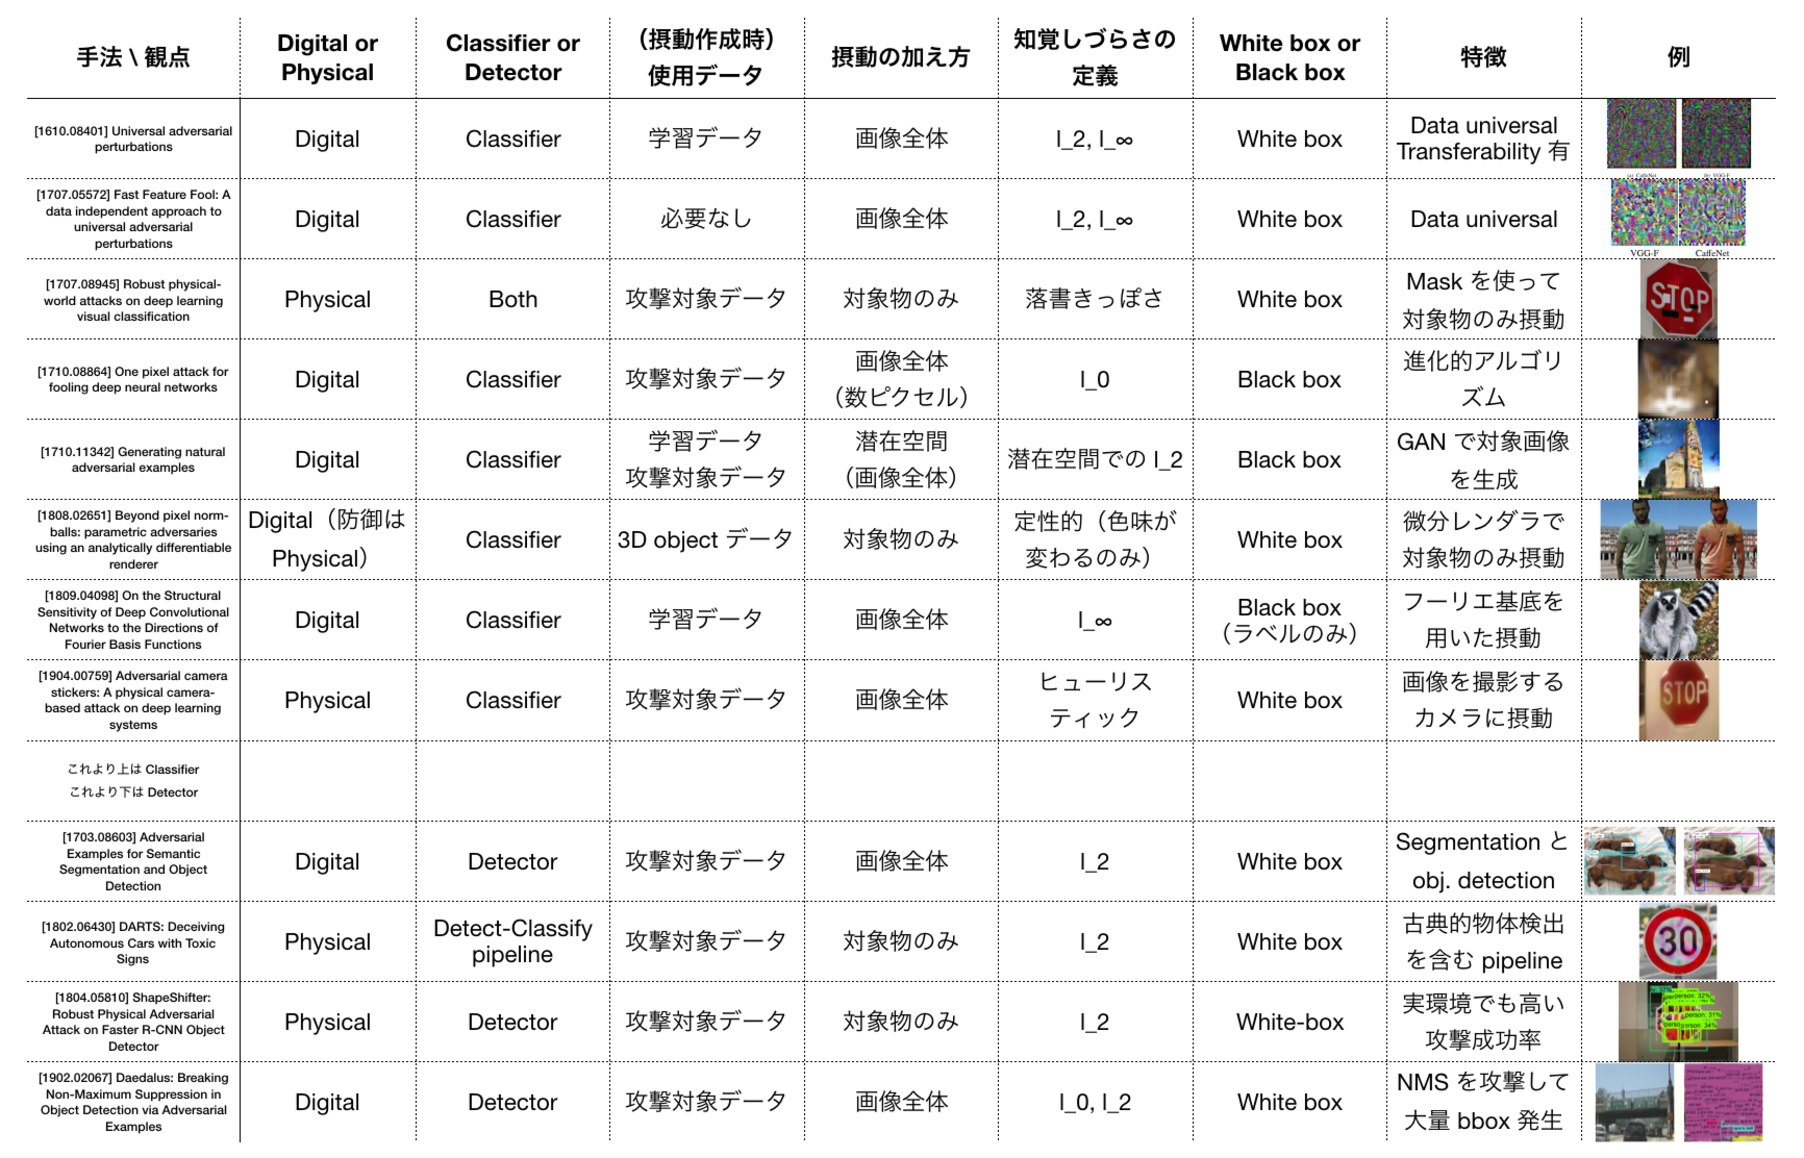
\includegraphics[width=16.0cm]{figures/attack-summary-table.pdf}
\end{center}
\caption{
本書で解説する攻撃手法の一覧とその特徴をまとめた表.
digital $\lor$ physical, classifier $\lor$ detector, 摂動作成時に使用するデータ, black box $\lor$ white box, 知覚しづらさの定義, 摂動の加え方, という観点で分類している.
個人的に重視している観点のため class ifier に対する手法と detector に対する手法を上下に分けて記載している.
文字が小さいため拡大して見ることを推奨.
}
\label{fig:attack-summary-table}
\end{figure}
%



\subsection{FGSM を基にした手法}
\label{subsec:fgsm-based}

\begin{table}[htbp]
\begin{center}
\begin{tabular}{|c|c|}
\hline
分類の観点 & この手法が該当するもの \\
\hline
Digital $\lor$ Physical & Digital \\
Classifier $\lor$ Detector & Classifier \\
摂動作成時に使用するデータ & 攻撃対象データ \\
摂動の加え方 & 画像全体 \\
知覚しづらさの定義 & $l_2$ もしくは $l_\infty$ \\
White box $\lor$ Black box & White box \\
\hline
\multicolumn{2}{|c|}{非公式実装: 検証実験のコードに含まれている} \\
\hline
\end{tabular}
\label{tb:fgsm-summary}
\end{center}
\end{table}

\ref{subsec:def-adv-examples} 節で既出であるが, adversarial examples を作成するための最も基本的な手法が FGSM である.
これは \cite{goodfellow2014explaining} によって提案された手法で, 一階微分に基づく手法であり広く使われている.

この手法は adversarial examples の初期に出たシンプルなものであり, この手法は多くの手法の基礎となったものである.
画像のピクセル値を任意に操作する Digital な攻撃で, 画像全体の情報を使ってラベルを予測する Classifier に対する攻撃である.
摂動は一枚の画像に対して対応する摂動を構築するようになっており, 画像と作成される adversarial example は一対一の関係にある.
摂動は画像全体に適用するので背景部分なども気にせず摂動を加えるようになっており, White box attack なのでモデルと loss function の情報を用いてモデルが誤認識しやすいように摂動を作成する.
人間にとっての知覚しづらさは摂動の $l_2$ や $l_{\infty}$ ノルムで測り, これらのノルムが小さければ摂動を加えた画像がその意味で元の画像から乖離が少なくなるため見分けがつきにくい, という方針である.
$l_{\infty}$ の方が定式化としてはすっきりとするため, $l_{\infty}$ の方を使うことが多い.

具体的な表式は式 \ref{eq:adv-fgsm} の繰り返しとなるが, adversarial examples の作り方は以下のようになっている.
%
\begin{eqnarray}
x_{\text{adv}} = x + \omega = x + \epsilon \cdot \text{sign} ( \nabla_x J (f, x, y_{\text{true}}) ).
\label{eq:adv-fgsm-again}
\end{eqnarray}
%
この手法が考案された背景は単純なものである.
重みベクトルを $w$ として $x_{\text{adv}}$ を以下のように分解することを考える.
%
\begin{eqnarray}
w^T x_{\text{adv}} = w^T x + w^T \omega.
\label{eq:adv_decompose}
\end{eqnarray}
%
一項目が摂動なしのもので二項目が摂動の効果であり, 摂動を小さく保ちつつ元の特徴からは大きく異なるものにしたいということを考えれば, $\epsilon$ の各要素の大きさは小さくしつつも $w^T$ との積は大きくするということになる.
各要素の大きさは $l_\infty$ で制限することにすると, この $\epsilon$ は $\epsilon = \epsilon \cdot \text{sign} (w)$ とするのがよいことが分かる.
このシンプルな考えをモデルに適用するには, 式 \ref{eq:adv-fgsm-again} のように loss function を $x$ で微分\footnote{
adversarial examples 作成時には重みベクトルは固定して, 変更するのは入力データである.
}して loss が大きくなるように正符号で元の $x$ に加えればよい (ただし $\epsilon > 0$ とする).
モデルの重みの更新の場合とは異なり, このデータの更新は一度だけ実施する.
この手法で構成された画像の例が図 \ref{fig:goodfellow-adv-example} である.
%
\begin{figure}[htbp]
\begin{center}
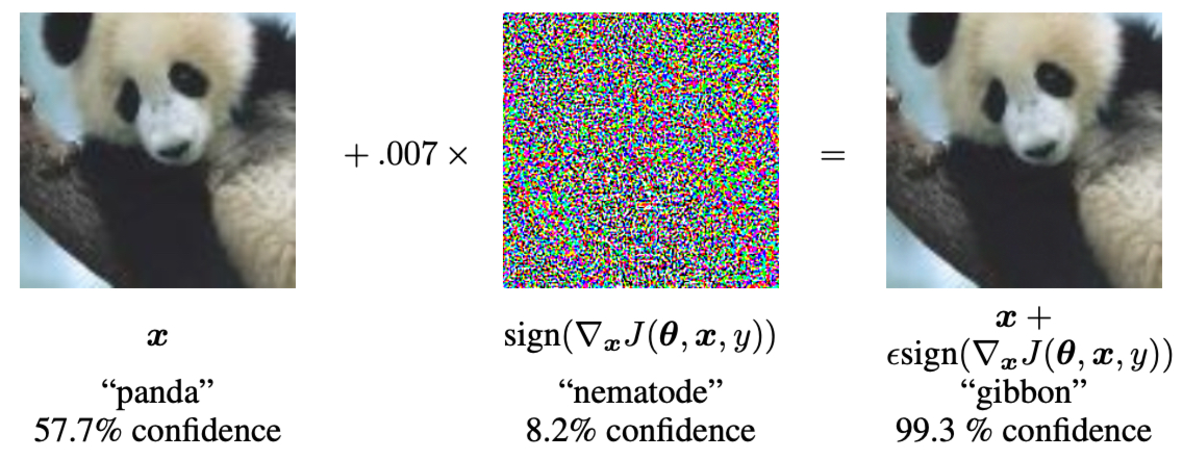
\includegraphics[width=12.0cm]{figures/goodfellow-adv-examples.pdf}
\end{center}
\caption{
FGSM で作成した adversarial examples の例.
攻撃対象としているモデルは GoogLeNet \cite{szegedy2015going} である.
左列が元画像, 中央列が作成した摂動, 右列が元画像に摂動を加えた画像である.
\textit{panda} と認識されていた画像が \textit{gibbon} (テナガザル) と誤認識されてしまっている.
図は \cite{goodfellow2014explaining} より引用.
}
\label{fig:goodfellow-adv-example}
\end{figure}
%

この構成法から明らかなように, この手法は white box attack であり, モデルの loss function とその微分情報がなければ使えないものである.
構成法がシンプルでありながら結果が興味深いものであり, 既存の DNN フレームワークで実装も容易であるため, その後の発展の礎になった手法であると共に現在もベースライン手法としてたびたび用いられる.

R+FGSM は FGSM にランダムなノイズの効果を入れることで後述する防御方法である adversarial training に有効な adversarial examples を作成しようとする手法である.
FGSM で作成した adversarial examples による loss function の形状は元データ近辺に局在していて大域的な最適化が困難になるため, ノイズを注入してそれを緩和するという目的で導入された.
まだ防御方法の紹介をしていないためここでは詳細は割愛するが, 手法としては以下のようにシンプルである.
%
\begin{eqnarray}
x_{\text{adv}} = x + \omega  = x + \alpha \cdot \text{sign} (\mathcal{N} (0^{m}, I^{m})) + (\epsilon - \alpha) \cdot \text{sign} (\nabla_x J (f_{\text{logit}}(x), y_{\text{true}})).
\label{eq:rfgsm}
\end{eqnarray}
%
ここで, $\mathcal{N} (0^{m}, I^{m})$ は $m$ 次元正規分布であり, $0 < \alpha < \epsilon$ である.
元論文では正規分布を用いているが, 符号のみが重要なので正負が等しい確率で得られればよいのでベルヌーイ分布や一様分布などでも同じ結果となる。

I+FGSM は元論文では PGD と呼称されている (本書では FGSM との関連性を明示するために I+FGSM と書く).
Iterative という名前から想像されるように, FGSM を繰り返し適用する手法となっている.
ただし, 繰り返し適用することで摂動が大きくなってしまう可能性があるため, 摂動が大きくなりすぎないように一定範囲に収まるように射影するというものになっている.
合計 $K$ 回の繰り返しをしてその途中の $t$ 回目の adversarial examples を $x_{\text{adv}}^t$ と書くとき, I+FGSM は以下のように書ける.
%
\begin{eqnarray}
\begin{aligned}
x_{\text{adv}}^{(0)} &= x \\
x_{\text{adv}}^{(t + 1)} &= x_{\text{adv}}^{(t)} + \alpha \cdot \text{sign} (\nabla_x J (f, x_{\text{adv}}^{(t)}, y_{\text{true}})) \\
x_{\text{adv}}^{(t + 1)} &= \text{clip} (x_{\text{adv}}^{(t + 1)}, x - \omega, x + \omega) \\
x_{\text{adv}} &= x_{\text{adv}}^{(K)}
\end{aligned}
\label{eq:ifgsm}
\end{eqnarray}
%
ここで, $\text{clip} (x, x_{\text{min}}, x_{\text{max}})$ は入力 $x$ を $[x_{\text{min}}, x_{\text{max}}]$ に射影する elementwise に適用される関数である.

MI+FGSM は I+FGSM の改良版であり, 前のステップでの微分情報に decay factor $\mu$ を掛けて momentum として使用して更新する手法である.
%
\begin{eqnarray}
\begin{aligned}
x_{\text{adv}}^{(0)} &= x \\
g^{(0)} &= 0 \\
g^{(t + 1)} &= \mu g^{(t)} + \frac{\nabla_x J (f, x_{\text{adv}}^{(t)}, y_{\text{true}})}{\|\nabla_x J (f, x_{\text{adv}}^{(t)}, y_{\text{true}})\|_1} \\
x_{\text{adv}}^{(t + 1)} &= x_{\text{adv}}^{(t)} + \alpha \cdot \text{sign} (g^{(t + 1)}) \\
x_{\text{adv}}^{(t + 1)} &= \text{clip} (x_{\text{adv}}^{(t + 1)}, x - \omega, x + \omega) \\
x_{\text{adv}} &= x_{\text{adv}}^{(K)}
\end{aligned}
\label{eq:mifgsm}
\end{eqnarray}
%
この手法は 2017 NIPS Adversarial Attacks Competition で一位を獲得した手法である.



\subsection{Universal adversarial perturbations}
\label{subsec:universal-adversarial}
%
\begin{table}[htbp]
\begin{center}
\begin{tabular}{|c|c|}
\hline
分類の観点 & この手法が該当するもの \\
\hline
Digital $\lor$ Physical & Digital \\
Classifier $\lor$ Detector & Classifier \\
摂動作成時に使用するデータ & 学習データ全体 \\
摂動の加え方 & 画像全体 \\
知覚しづらさの定義 & $l_2, l_{\infty}$ \\
White box $\lor$ Black box & White box \\
\hline
\multicolumn{2}{|c|}{公式実装: \href{https://github.com/LTS4/universal}{https://github.com/LTS4/universal}} \\
\hline
\end{tabular}
\label{tb:universal-adversarial-summary}
\end{center}
\end{table}
%

これは \cite{moosavi2017universal} によって提案された手法であり, 概要は図 \ref{fig:universal-adversarial-summary} のようになっており, 様々なクラスの画像に対して単一の摂動を加えることで異なるクラスに誤認識させることに成功している.
%
\begin{figure}[htbp]
\begin{center}
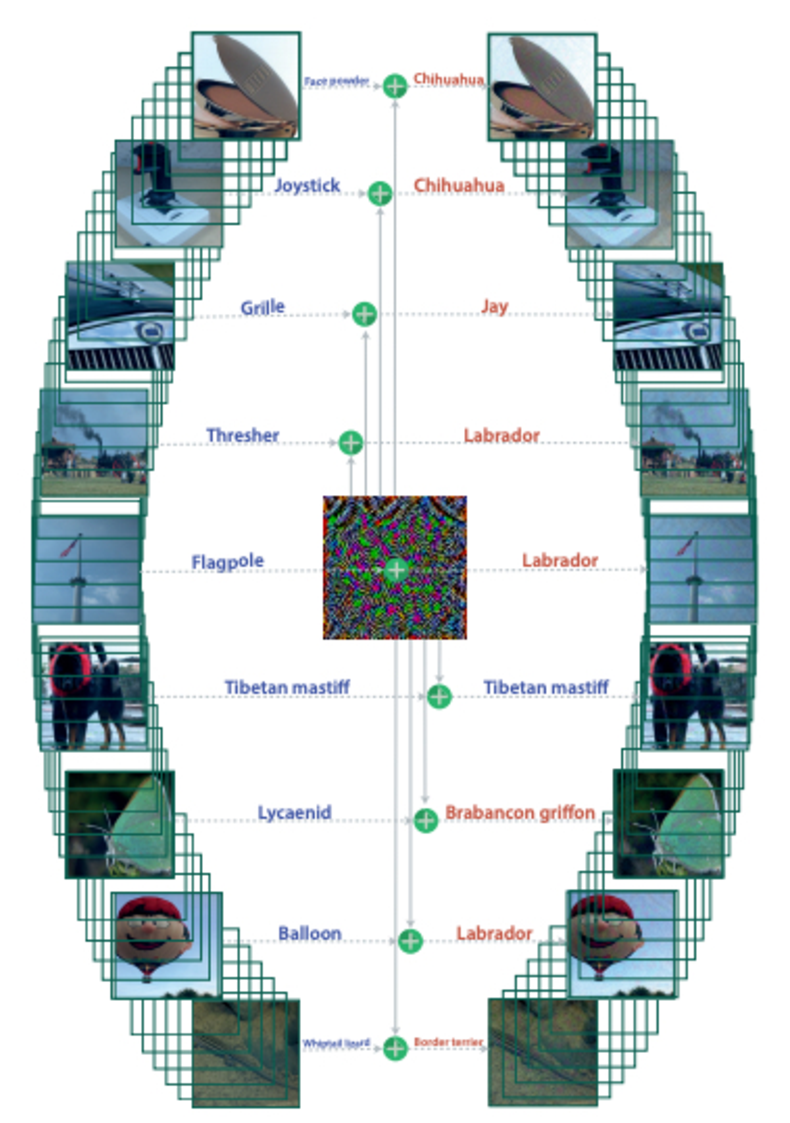
\includegraphics[width=10.0cm]{figures/universal-adversarial-summary.pdf}
\end{center}
\caption{
手法の概要.
左側の画像とラベルが元画像とモデルによって予測される正しいラベルで, 中央にある単一の摂動をそれぞれの画像に加えることで, 右側の画像になり予測ラベルも変わる (赤字は正しくないラベルで誤認識されたことを示す).
図は \cite{moosavi2017universal} より引用.
}
\label{fig:universal-adversarial-summary}
\end{figure}
%

この手法はの特徴は摂動を作成する際に学習データ全体を使用することにあり, 多様なデータを用いることで, 攻撃時にも多様なデータに対して有効な普遍的な一つの摂動を作成することに成功している.
基本的なアイデアは, あるデータに対して誤認識させるために識別領域を超えるような摂動を作成し, それを一定の大きさに保ちながら各データに対して繰り返し適用するというものである.
それ以外の観点は FGSM と同様である.

この手法が登場するまでは, 一枚の攻撃対象となる画像データに対して摂動を作成するというものが殆どだったが, この手法が目指すところは摂動として普遍的 (ここでは攻撃対象となる画像に依らないという意味) なものの作成である.
実現したい状況を定式化すると以下のようになる.
$x$ は集合 $\mathcal{X}$ に属する様々なデータとなるが, 摂動である $\omega$ は $x$ に依らない単一の量であることに注意されたい.
%
\begin{eqnarray}
f_{\text{label}} (x + \omega) \neq f_{\text{label}} (x) \ \ \text{for "most" } x \in \mathcal{X}.
\label{eq:universal-adversarial-formulation}
\end{eqnarray}
%
論文では $x \sim  \mu$ としてデータ $x$ を生成する確率分布 $\mu$ を用いているが, 当然これは直接は扱えないものであるため, ここでは入力データ集合に置き換えている.
この段階では摂動の大きさに制限がないのと, 「most」 の意味するところが抽象的であるので, それを明示的に取り入れるため以下の条件を課す.
%
\begin{enumerate}
  \item $\|\omega\|_{p} \leq \epsilon.$
  \item $\text{Err}_{x \in \mathcal{X}} \left( f_{\text{label}} (x + \omega) \neq f_{\text{label}} (x)  \right) \geq 1 - \delta.$
\end{enumerate}
%
2 つ目の条件は誤認識させる割合が $1 - \delta$ であることを意味している.
目的はこの $(\epsilon, \delta)$ として共に小さい値を実現するようなアルゴリズムを構築すること, と言い換えることができる.

そうは言っても使用する技術的な道具は FGSM の場合とそう大きくは変わらない.
アルゴリズム \ref{alg:universal-adversarial-alg} に全体像を示す.
摂動を更新する際のコアとなる手法は FGSM などの先行研究の手法を用いるものになっており, 論文では DeepFool \cite{moosavi2016deepfool} を用いている\footnote{
これは FGSM を iterative に改良した手法で, 各ステップで勾配情報から摂動 $\omega_i$ を作成し, 次のステップで $x + \omega_i$ で同様の操作を実施して最終的に $\omega = \sum \omega_i$ とする.
I+FGSM との違いは I+FGSM は毎回 $\omega$ 全体を更新しているが, DeepFool では各ステップの変位を残しておいて最後にそれを足すという点にある.
攻撃性能は I+FGSM の方が高いが, ベースライン手法として DeepFool もたびたび用いられる.
}.
各データ毎に摂動を作成してそれを加えていくことで摂動の大きさが増大していく可能性があるため, $l_p$ ノルム の値が $\epsilon$ 以下という条件の下で $l_2$ ノルムの意味で最適な摂動に近づくように制限を加えている.
あとはこの手続きを所望の誤認識率を達成するまで繰り返せばよい.
注意すべき点として, このアルゴリズムはモデルに依存するのはもちろんのこと, データ集合 $\mathcal{X}$ を固定してもループの順番によって最終的に得られる摂動が変わるということが挙げられる.
%
\begin{algorithm}
\caption{Universal Adversarial Perturbations のアルゴリズム}
\label{alg:universal-adversarial-alg}
\begin{algorithmic}[1]
    \State Input: データ集合 $\mathcal{X}$, モデル $f_{\text{label}}$, $l_p$ノルムとその大きさの制限 $\epsilon$, 誤認識率を測る
    $\delta$
    \State Output: 摂動 $\omega$
	\State 摂動を初期化: $\omega \leftarrow 0$
	\While {$\text{Err}_{x \in \mathcal{X}} \left( f_{\text{label}} (x + \omega) \neq f_{\text{label}} (x)  \right) \leq 1 - \delta.$}
	\For {各データ $x_i \in \mathcal{X}$}
	\If {$f_{\text{label}} (x_i + \omega) = f_{\text{label}} (x_i)$}
	\State 誤認識をさせるために必要な最小限の摂動を計算 (FGSM などの先行研究の手法を用いる): $\Delta \omega_i \leftarrow \argmin_{r} \left[\|r\|_2\right] \ \text{s.t.} \  f_{\text{label}} (x_i + \omega + r) \neq f_{\text{label}} (x_i).$ 
	\State 摂動を更新: $\omega \leftarrow \argmin_{\omega'} \left[ \|(\omega + \Delta \omega_i) - \omega'\|_2 \right] \ \text{subjet to} \ \|\omega'\|_p \leq \epsilon.$
	\EndIf
	\EndFor
	\EndWhile
\end{algorithmic} 
\end{algorithm}
%

ILSVRC2012 \cite{russakovsky2015imagenet} データを用いた実験結果を見ていこう.
実験に使用しているモデルは以下の通りで, 論文出版時の主要なモデルが取り上げられている.
%
\begin{itemize}
  \item CaffeNet \cite{jia2014caffe}
  \item VGG-F \cite{chatfield2014return}
  \item VGG \cite{simonyan2014very}
  \item GoogLeNet \cite{szegedy2015going}
  \item ResNet \cite{he2016deep}
\end{itemize}
%

まずは摂動を作成するために 10,000 件のデータを用いて, 検証用に 50,000 件使用した結果が図 \ref{fig:universal-adversarial-result-table} である.
どのモデルにおいても $\mathcal{X}$ でも検証用データでも同程度の誤認識率となっており, 作成した摂動は $\mathcal{X}$ のみに過学習しているわけではないことが分かる (元が同じデータセットなのでそこまで強い主張にはなり得ないが).
また, $l_2, l_\infty$ ノルムのどちらが適しているかはモデルによって異なる.
大きな傾向として, モデルの層の数などが少ない簡単なモデルの方が誤認識率が高いことが伺える.
%
\begin{figure}[htbp]
\begin{center}
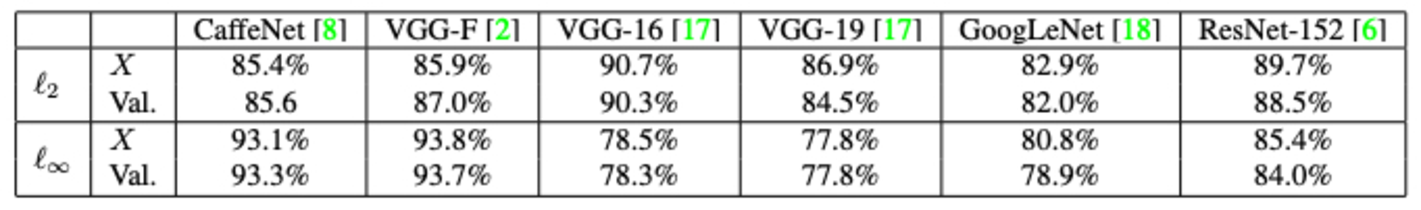
\includegraphics[width=14.0cm]{figures/universal-adversarial-result-table.pdf}
\end{center}
\caption{
摂動を作成したデータと検証用のデータそれぞれでの誤認識率を比べたもの.
$l_2$, $l_{\infty}$ の制限としてそれぞれ $\epsilon = 2000, \epsilon = 10$ を用いている.
図は \cite{moosavi2017universal} より引用.
}
\label{fig:universal-adversarial-result-table}
\end{figure}
%

次にモデル毎に得られた普遍的な摂動を示したものが図 \ref{fig:universal-adversarial-perturbations-models} である.
モデル毎に人間にとっても大きく見た目が異なる摂動が得られている.
%
\begin{figure}[htbp]
\begin{center}
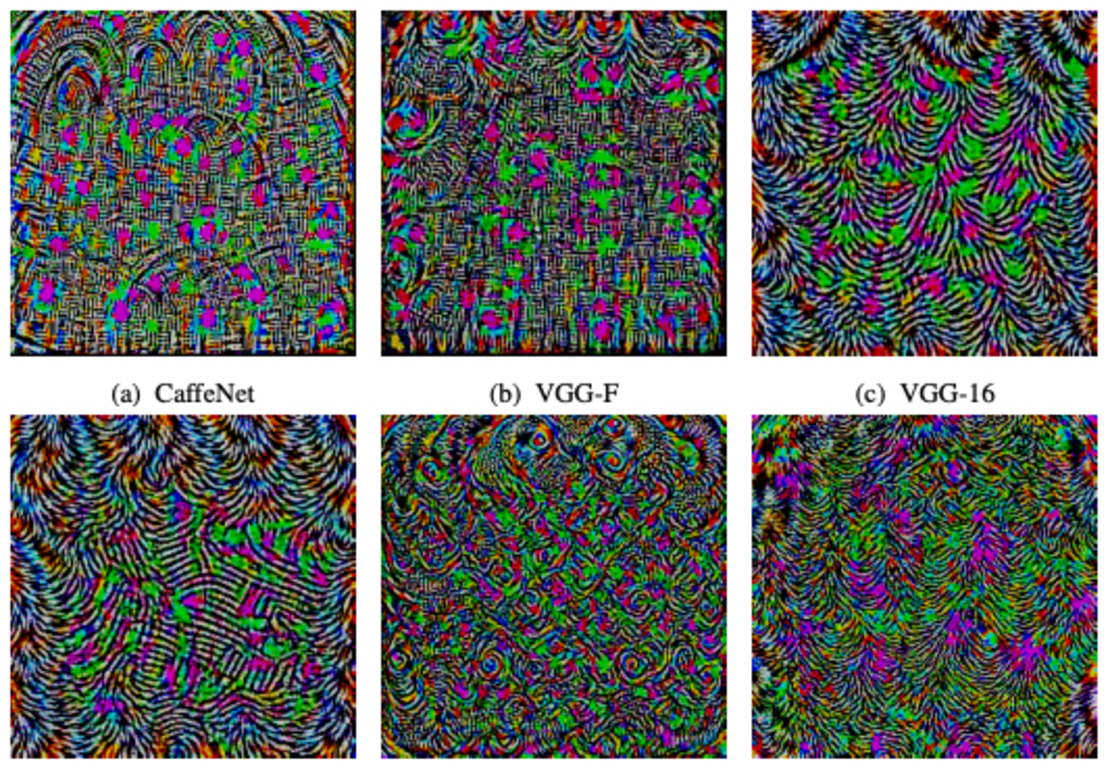
\includegraphics[width=10.0cm]{figures/universal-adversarial-perturbations-models.pdf}
\end{center}
\caption{
モデル毎に得られた普遍的な摂動.
図は \cite{moosavi2017universal} より引用.
}
\label{fig:universal-adversarial-perturbations-models}
\end{figure}
%

この手法はデータの順番に依存するものであることを言及していたが, データ順を変えた場合に結果がどう変わるかを示したものが図 \ref{fig:universal-adversarial-perturbations-shuffle} である。
モデルは GoogLeNet を使用していて, 人間の目には似通った模様に見えるが, 正規化した内積の値は 0.1 以下であり, 普遍的な摂動はデータ順に依存して unique なものではないことが示されている.
%
\begin{figure}[htbp]
\begin{center}
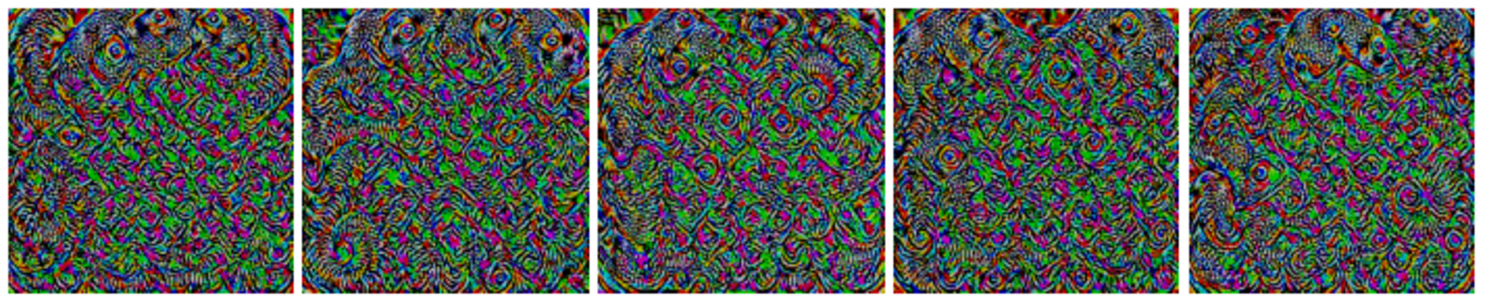
\includegraphics[width=14.0cm]{figures/universal-adversarial-perturbations-shuffle.pdf}
\end{center}
\caption{
データ順をシャッフルし GoogLeNet で異なる普遍的な摂動を求めた結果.
それぞれの正規化した内積を計算すると値は 0.1 以下となり, 人間の目では似通って見えるが異なる摂動になっている.
図は \cite{moosavi2017universal} より引用.
}
\label{fig:universal-adversarial-perturbations-shuffle}
\end{figure}
%

ここまでの結果で, 提案手法の目的であった個別のデータに依らない普遍的な摂動というのが確かに構築できる (しかし unique ではない) ということが示された.
それだけに留まらず, あるモデルで作成した摂動が他のモデルでも一定度の有効性があることも示されている.
その結果が図 \ref{fig:universal-adversarial-transferability} であり, このように別モデルに対しても有効であることを adversarial examples に transferability があると言う.
この論文が発表されて以降, adversarial examples の transferability に関して様々な進展が報告されるようになった.
モデルの構造が似通っていると高い transferability を達成していることが見て取れる.
%
\begin{figure}[htbp]
\begin{center}
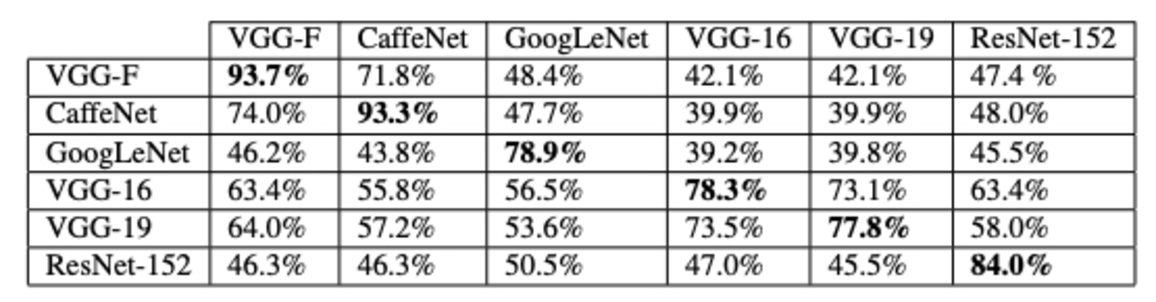
\includegraphics[width=14.0cm]{figures/universal-adversarial-transferability.pdf}
\end{center}
\caption{
adversarial examples の transferablity を調べた結果.
各行が普遍的な摂動を作成するのに使用したモデルで, 各列が誤認識率を計算したモデルになっている.
図は \cite{moosavi2017universal} より引用.
}
\label{fig:universal-adversarial-transferability}
\end{figure}
%

なぜ単一の普遍的な摂動が有効なのかというのが疑問として残るが, 論文では識別境界付近は比較的少数のベクトルで span される低次元空間で記述されているのではないかという仮説に基づいてデータ点での識別境界への法線ベクトルの解析を実施している.
CaffeNet において, 以下で定義される識別境界への法線ベクトルを集めた行列を求める.
%
\begin{eqnarray}
N = \left[ \frac{\omega(x_1)}{\|\omega(x_1)\|_2}, \dots, \frac{\omega(x_{|\mathcal{X}|})}{\|\omega(x_{|\mathcal{X}|})\|_2} \right] \ \text{where} \ \argmin_{\omega} \left[ \|\omega\|_2 \right] \ \text{s.t.} \ f_{\text{label}} (x + \omega) \neq f_{\text{label}} (x).
\label{eq:universal-adversarial-normalvect}
\end{eqnarray}
%
この行列の特異ベクトルと単位球からランダムサンプルした特異ベクトルを比較する.
その結果が図 \ref{fig:universal-adversarial-singular-values} で, 確かに識別境界への法線ベクトルは少数のベクトルの寄与が大きく有効次元が低いことが示されている.
この論文ではこのようなある種の状況証拠のような解析までしか実施されていないが, 後の論文で識別境界付近の曲率に注目し, 線形もしくは条件付きの非線形の識別境界の場合に普遍的な摂動に弱いことが報告されている\cite{moosavi2017analysis}.
%
\begin{figure}[htbp]
\begin{center}
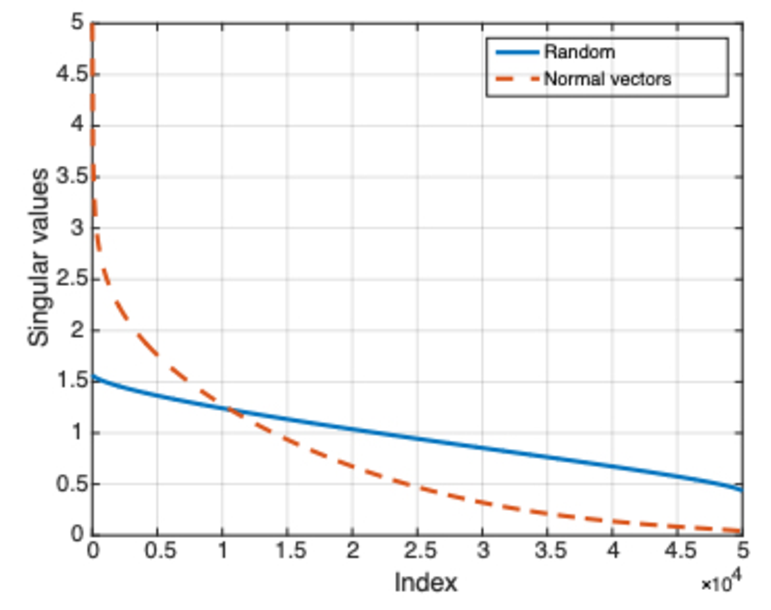
\includegraphics[width=8.0cm]{figures/universal-adversarial-singular-values.pdf}
\end{center}
\caption{
識別境界への法線ベクトルをまとめた行列の特異値分布と単位球からランダムサンプルした場合の特異値分布を比較した結果.
縦軸は特異値の大きさで横軸は特異値を大きい順に並べたときの index である.
識別境界付近の空間が少数の特異ベクトルで記述されていることを示している.
図は \cite{moosavi2017universal} より引用.
}
\label{fig:universal-adversarial-singular-values}
\end{figure}
%

その他にも, 誤認識されるクラスは等しく分布するのではなく特定のクラスに偏る傾向にあるという性質とそのグラフ理論的な解析の方向性も言及されているが, この点に関してその後詳しく調べられているかは著者は知らない.

この手法は示唆に富むものであったので, その後の様々な発展につながっている.
特に, adversarial examples の transferability に関して, 現実的に攻撃する際には (攻撃対象のモデルの情報は取得できないことが殆どなので)  black box attack を用いる必要があるが, 手元で white box の手法で作成した adversarial examples を攻撃に転用するのが主流となった.



\subsection{Fast Feature Fool: A data independent approach to universal adversarial perturbations}
\label{subsec:fast-feature}
%
\begin{table}[htbp]
\begin{center}
\begin{tabular}{|c|c|}
\hline
分類の観点 & この手法が該当するもの \\
\hline
Digital $\lor$ Physical & Digital \\
Classifier $\lor$ Detector & Classifier \\
摂動作成時に使用するデータ & モデル情報のみでデータは必要なし \\
摂動の加え方 & 画像全体 \\
知覚しづらさの定義 & $l_{\infty}$ \\
White box $\lor$ Black box & White box \\
\hline
\multicolumn{2}{|c|}{公式実装: \href{https://github.com/val-iisc/fast-feature-fool}{https://github.com/val-iisc/fast-feature-fool}} \\
\hline
\end{tabular}
\label{tb:fast-feature-summary}
\end{center}
\end{table}
%

これは \cite{mopuri2017fast} によって提案された手法であり, データに依らずにモデルの各層の出力の平均値が大きくなるような摂動を作成することで誤認識を引き起こす手法である.

摂動作成時に使用するデータ以外は FGSM や Universal Adversarial Perturbation と変わらないが, 摂動を作成する際にモデルの情報のみを使いデータを全く使わないのが特徴である.
モデルによる予測はある層の出力に変換を施してそれを次の層に渡してということを繰り返していくが, 各層の出力が入力データに関わらずに大きくなるような摂動が作成できれば, 入力データの特徴が無視されるほど摂動の影響が大きくなり, 誤認識を引き起こすことが可能になると考えられる.
そのような摂動は学習済みモデルがあれば作成することができるので, それを実際にやってみたのがこの手法となる.

摂動を適当に初期化して, 層 $i$ の出力の平均を $\bar{l}_i$ として以下のように loss function を設定する.
%
\begin{eqnarray}
J(f, \omega) = - \log \left(\prod_{i = 1}^{\text{\# of layers}} \bar{l}_i (\omega) \right) \ \text{s.t.} \ \|\omega\|_p < \epsilon.
\label{eq:fast-feature-loss}
\end{eqnarray}
%
出力は基本的には ReLU の出力を使用することを想定しているので非負であり, fully connected layer より手前の convolutional layer を $i$ として採用している\footnote{
実装を見ると途中の pooling layer も含めているように読み取れるのでその限りではない.
詳しくは実装を参照のこと.
}.

提案手法としては以上で, あとは Universal Adversarial Perturbations と同様に ILSVRC2012 と各種モデルを使った実験に入る.
摂動の大きさとして $\epsilon = 10$ を用いており, これは Universal Adversarial Perturbations と同じ値である.
まず, ILSVRC2012 で学習した各モデルから得られた摂動は図 \ref{fig:fast-feature-perturbations} である.
Universal Adversarial Perturbations の結果と比べるとより特定の模様が強調されているようにも見えるが, そこに何かしらの意味があるのかは論文では言及されておらず, 著者にも分からない.
%
\begin{figure}[htbp]
\begin{center}
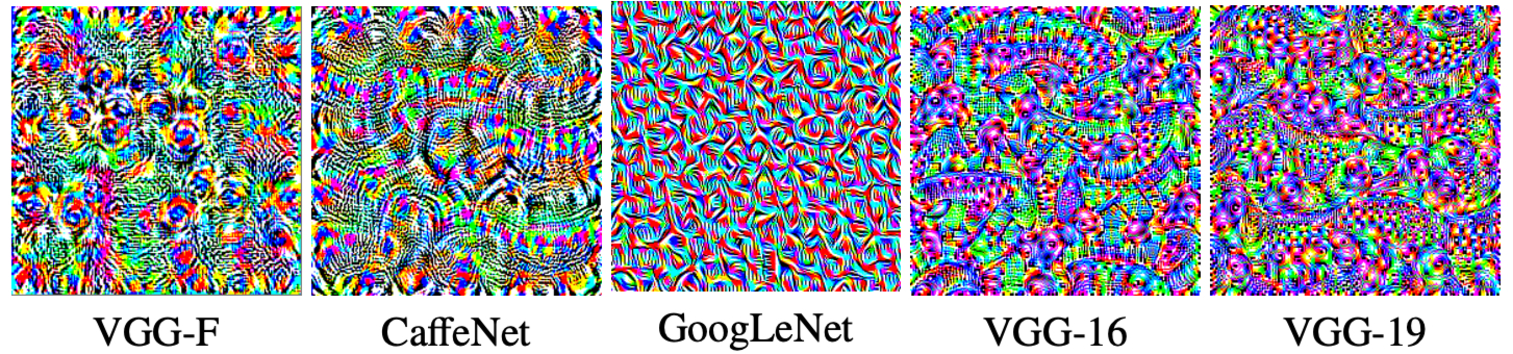
\includegraphics[width=14.0cm]{figures/fast-feature-perturbations.pdf}
\end{center}
\caption{
モデル毎に得られた摂動.
図は \cite{mopuri2017fast} より引用.
}
\label{fig:fast-feature-perturbations}
\end{figure}
%

得られた摂動を用いて誤認識率を調べたものが図 \ref{fig:fast-feature-transferability} である.
具体的なデータを使っていないため Universal Adversarial Perturbations よりは誤認識率 (図 \ref{fig:universal-adversarial-transferability} を参照) が低くなっているが, それでも高い誤認識率を達成していることが示されている.
%
\begin{figure}[htbp]
\begin{center}
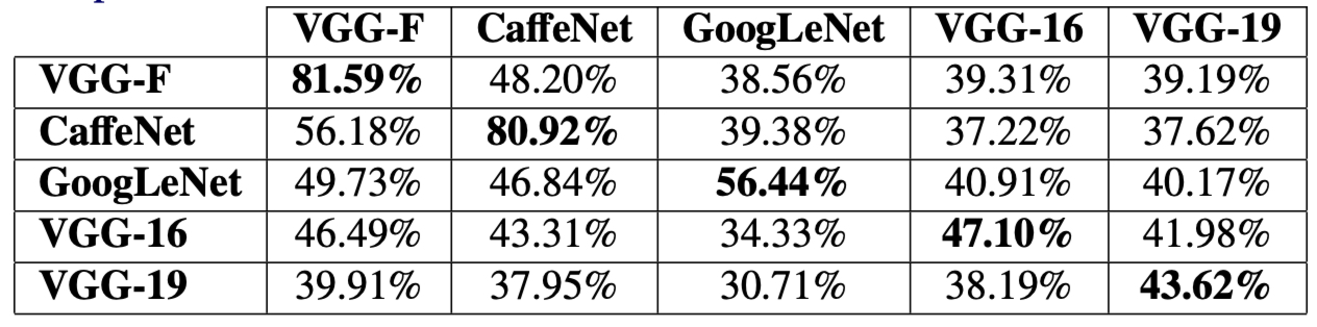
\includegraphics[width=14.0cm]{figures/fast-feature-transferability.pdf}
\end{center}
\caption{
ILSVRC2012 で学習したモデルから作成した摂動を用いて, 検証用のデータで誤認識率を調べた結果.
各行が摂動を作成したモデルで, 各列が誤認識率を評価したモデルになっている.
図は \cite{mopuri2017fast} より引用.
}
\label{fig:fast-feature-transferability}
\end{figure}
%

GoogLeNet で得られた摂動を用いて予測結果がどのように変化するかをサンプリングしたものが図 \ref{fig:fast-feature-examples} である.
拡大して見ることで確かに摂動が載っていることが分かる.
%
\begin{figure}[htbp]
\begin{center}
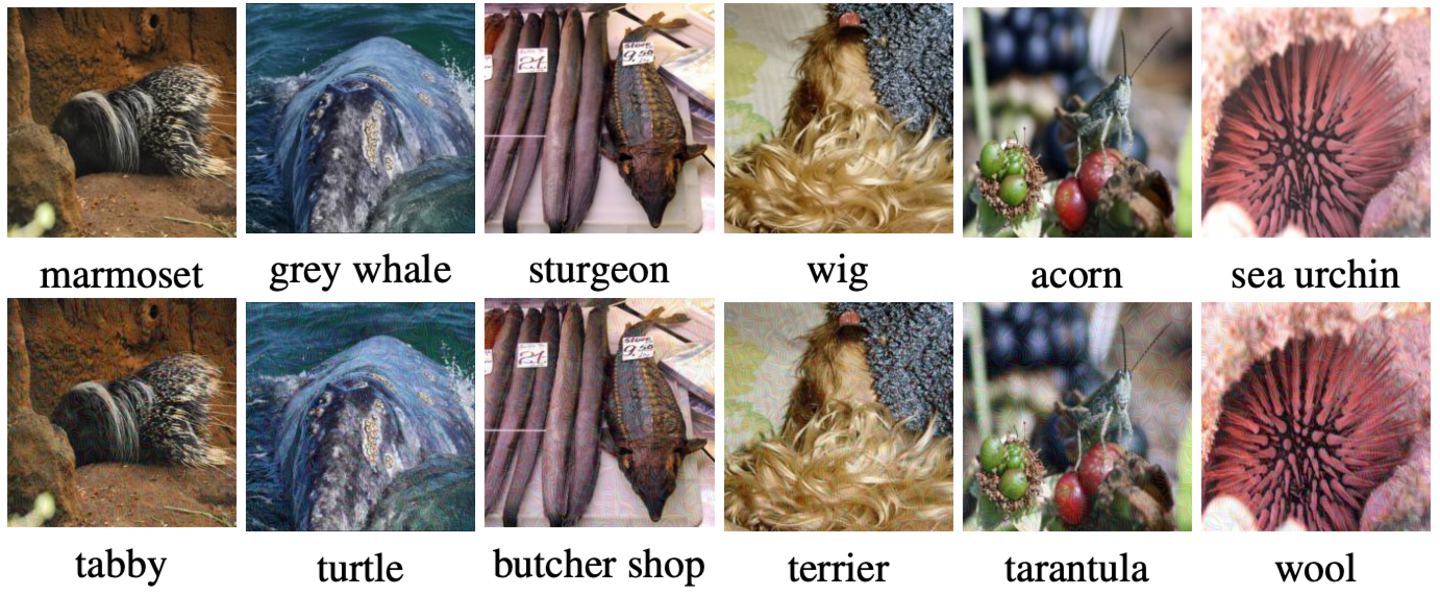
\includegraphics[width=14.0cm]{figures/fast-feature-examples.pdf}
\end{center}
\caption{
GoogLeNet における具体例.
上の行が元データと (正しく予測されている) ラベルで, 下の行が adversarial examples と誤認識されたラベルである.
図は \cite{mopuri2017fast} より引用.
}
\label{fig:fast-feature-examples}
\end{figure}
%

この論文では新たに adversarial examples のデータ間の transferability についても検証している.
具体的には ILSVRC2012 で学習したモデルで作成した摂動を Places-205 \cite{zhou2016places} の検証用データに加えて, Places-2015 で学習したモデルがどれくらい誤認識するかを調べている.
結果が図 \ref{fig:fast-feature-data-transferability} であり, ある程度はデータ間の transferability が存在することが示されている.
提案手法はかなり誤認識率が低いが Universal Adversarial Perturbations では高いことから, 提案手法はかなりデータに特化した摂動で Universal Adversarial Perturbations に関してはある程度物体の普遍的な特徴に対する摂動となっていると考えられる.
%
\begin{figure}[htbp]
\begin{center}
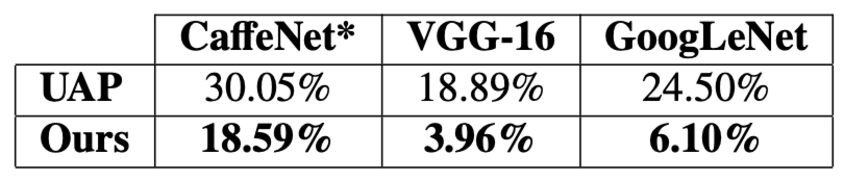
\includegraphics[width=10.0cm]{figures/fast-feature-data-transferability.pdf}
\end{center}
\caption{
adversarial examples に対してデータの transferability を調べた結果.
ILSVRC2012 で学習したモデルで作成した摂動を使って Places-205 のデータセットで検証をしている.
UAP は Universarial Adversarial Perturbations を意味しており, CaffeNet のスターは実際には誤認識率を計算する際に AlexNet を用いていることを意味している (2 つのアーキテクチャは似ているが少し異なっている).
図は \cite{mopuri2017fast} より引用.
}
\label{fig:fast-feature-data-transferability}
\end{figure}
%

この手法は摂動作成時はデータを用いないという点で興味深いものだが, 学習に用いたデータへの依存性が強い.
このような研究と Universal Adversarial Perturbations と合わせることで, 様々な transferability の可能性が認識されるようになった.



\subsection{Robust Physical-World Attacks on Deep Learning Models}
\label{subsec:robust-physical}
%
\begin{table}[htbp]
\begin{center}
\begin{tabular}{|c|c|}
\hline
分類の観点 & この手法が該当するもの \\
\hline
Digital $\lor$ Physical & Physical \\
Classifier $\lor$ Detector & Classifier (後に Detector にも有効であることを示した) \\
摂動作成時に使用するデータ & 攻撃対象クラスのデータ 1 枚 \\
摂動の加え方 & 対象物のみ \\
知覚しづらさの定義 & 落書きっぽさ \\
White box $\lor$ Black box & White box \\
\hline
\multicolumn{2}{|c|}{公式実装: \href{https://github.com/evtimovi/robust_physical_perturbations}{https://github.com/evtimovi/robust\_physical\_perturbations}} \\
\hline
\end{tabular}
\label{tb:robust-physical-summary}
\end{center}
\end{table}
%

これは \cite{eykholt2018robust} によって提案された手法であり, 概要は図 \ref{fig:robust-physical-summary} のようになっており, 止まれの標識を速度制限の標識に誤認識させるような摂動を作成している.
%
\begin{figure}[htbp]
\begin{center}
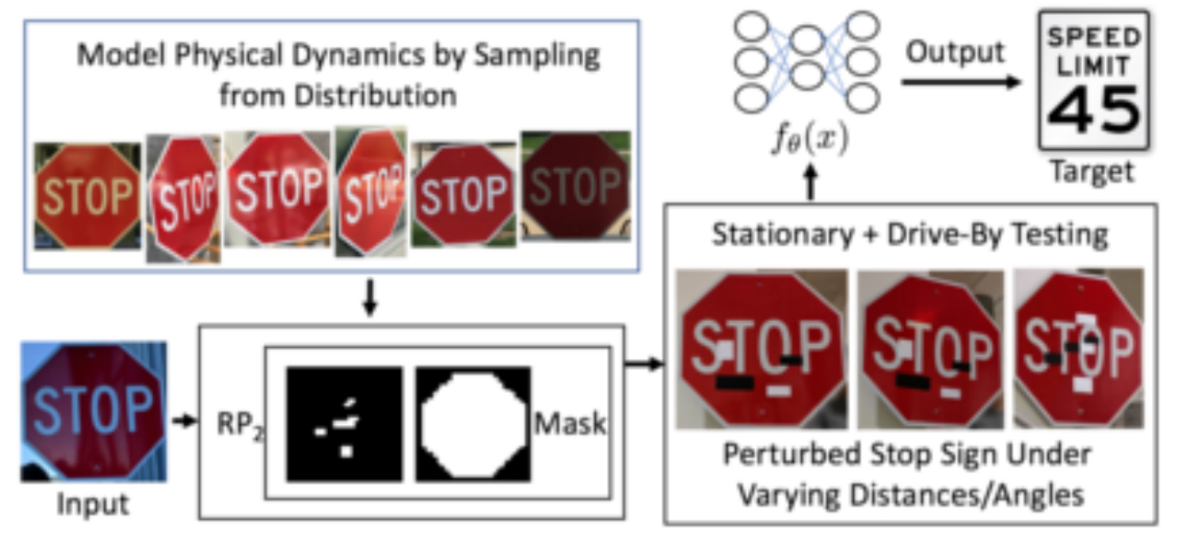
\includegraphics[width=12.0cm]{figures/robust-physical-summary.pdf}
\end{center}
\caption{
手法の概要.
標識のみに摂動を加えるような mask を作成し, 角度や明るさなどの条件を変更するような変換を適用したデータを用いて誤ったラベルに対する誤差が小さくなるような摂動を作成する.
図は \cite{eykholt2018robust} より引用.
}
\label{fig:robust-physical-summary}
\end{figure}
%

この手法は physical な攻撃であり, 標識に摂動を加えた画像をプリントしてそれを実際の標識に上から貼るというような手法になっている (本当に標識の上に印刷物を貼るのは違法なので, 実験では印刷物を室外環境で適当なところに貼って撮影して評価している).
摂動の作成はデジタル上で実施して, それをプリントして使用するため, 摂動作成時にはプリンターで実現可能な色味にできるだけ近づけるような拘束条件も導入している.

この攻撃の対象は classifier のみで画像中に単一の標識のみが映っているという状況を想定しており, そのため扱うデータも標識のみを切り出したものを使用する.
この論文の手法を detector にも適用できるように発展させた technical note を publish している \cite{eykholt2017note}.
この technical note では図 \ref{fig:robust-physical-detector} のようにある標識を別の標識に誤認識させるという手法ではなく標識を認識させず別の物体に誤認識させる手法だが, このような発展を通じて detector にも有効な adversarial examples が数多く報告されるようになってきている.
%
\begin{figure}[htbp]
\begin{center}
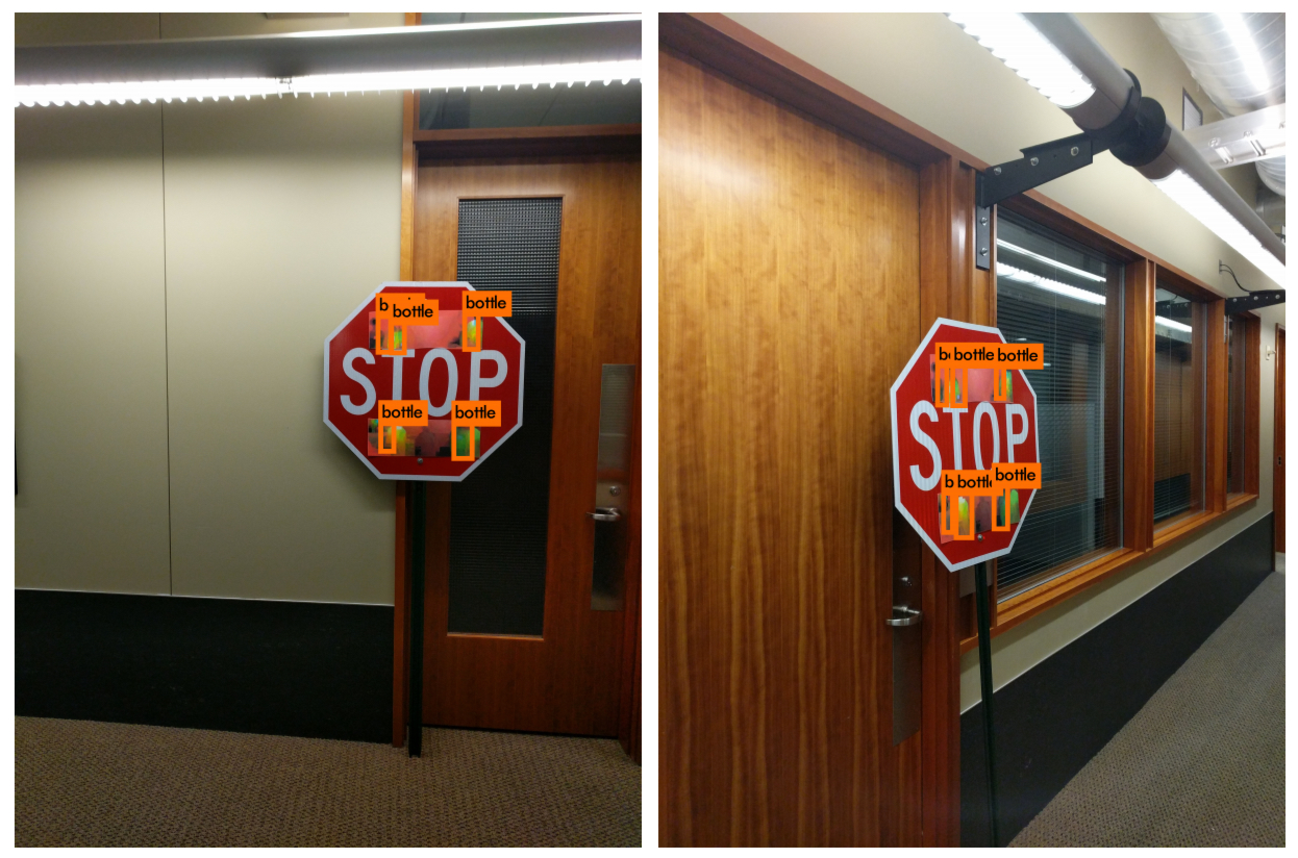
\includegraphics[width=12.0cm]{figures/robust-physical-detector.pdf}
\end{center}
\caption{
提案手法を detecotr に適用した結果.
図は \cite{eykholt2017note} より引用.
}
\label{fig:robust-physical-detector}
\end{figure}
%

摂動を作成する時は攻撃対象となるクラスの画像を一枚使用する.
道路標識は色々な距離や角度から撮影されるため, 摂動はそのような状況でも効果を発揮する必要がある.
そのため, その一枚に幾何学変換や輝度変換などを加えてデータセットを構築し, 対象となるクラスに有効な一つの摂動を作成する.
一クラスに対して一つの adversarial example を作るというものになっている.

この手法は white box に属するもので, モデルと loss function を与えて, loss function の値に基づいてモデルが誤認識をしやすいようにデータに摂動を加えていく.
標識外の部分に摂動を加えても撮影条件が変わればその効果は期待できないため, この手法では摂動を作成する際に標識以外の部分に mask  (この手法は攻撃対象のクラスの画像が一枚あれば作成できるため, それに合わせた mask を事前に準備している) を加えて標識部分だけで摂動を作成するようにしている.

知覚しづらさとして, 標識に落書きをしたような摂動になるために人間が adversarial examples と気付きにくいだろうというアイデアを採用している.
摂動自体は $l_1$ や $l_2$ ノルムを使って構築していくが, 様々な物理的環境で有効な摂動を作ろうとするとどうしても元画像からの差分は目につくようになる.
標識にスプレーなどで落書きをしたように見えるので知覚しづらい, というのはやや詭弁にも聞こえるが発想自体はなかなか面白いものであり, この考え方を推し進めて虫がついてるように見えるという摂動が考案 \cite{yakura2019generate} されていたりする.

mask を $M_x$ とし, $X^V$ を対象のクラスの一枚の画像に変換を加えて作成した集合とし, $T_i$ を $x_i$ を作成するために適用した変換をマスキングした摂動に変換する関数 (例えば元の 1 枚の画像に回転を加えたなら摂動にも同じ回転を加える) とすると, loss function は以下のように書ける.
%
\begin{eqnarray}
\argmin_{\omega} \left[ \lambda \| M_x \cdot \omega \|_p + NPS + \mathbb{E}_{x_i \sim X^V} J (f, x_i + T_i (M_x \cdot \omega), y_{\text{atk-tgt}}) \right].
\label{eq:robust-physical-loss}
\end{eqnarray}
%
ここで, $NPS$ は Non-Printability Score で, プリンターに出力可能な RGB の組を集めた集合を $P$ とし, $R(\omega)$ を各ピクセルでの摂動の RGB の組を集めて unique なもののみを対象とする集合とすると, 以下のように定義される.
%
\begin{eqnarray}
NPS = \sum_{\hat{p} \in R(\omega)} \prod_{p' \in P} |\hat{p} - p'|.
\label{eq:nps}
\end{eqnarray}
%
記法が少し独特だが, 難しいことは言っていない.
各ピクセルで RGB の組が得られるのでそれを全部集めてきて色の種類のみに注目するように unique な組だけを残して $R(\omega)$ を作り, プリント可能な RGB の組を集めた $P$ のどれかには近づくようにするというものである.
論文ではこれを fabrication error と呼んでいる.

式 \ref{eq:robust-physical-loss} の各項の意味を考えると, 第一項は mask をかけてはいるが摂動を $l_p$ ノルムの意味で小さく保つようにしているだけで, 第二項は NPS でプリンターがプリント可能な色にできるだけ近づくように寄せる効果があり, 第三項は正しいラベルではなく $y_{\text{atk-tgt}}$ に間違えさせるように loss の値を小さくするようにする FGSM と同様の項である.
ただし, $x_i$ は元画像から様々な変換を適用して生成するため, 摂動もそれと同じ変換を適用する必要があり, それが $T_i$ である (この $T_i$ は $x_i$ を生成するために定めた変換そのものなので, そのまま使い回せばよい).
これにより, 対象物を撮影する際の距離や角度や輝度が変わったときに, 摂動を同じように変更することで常に摂動が誤認識に導くような働きをするように仕向けることができる.

理論的な内容に関しては以上で, あとは標識データセットである LISA \cite{mogelmose2012vision} と GTSRB \cite{stallkamp2012man} を用いた実験に移る.
モデルはそれぞれに対して CNN を用いているが, どちらのデータセットもテストデータでの正答率が 90\% を上回るモデルを容易に構築でかつ結果がモデルの詳細にそれほど依らないため, モデルのアーキテクチャに関してはここでは割愛する\footnote{
adversarial examples の実験では ResNet のようなよく使われるアーキテクチャや, 特別な工夫が施されていないシンプルなモデルを用いることが多い.
モデルの詳細なアーキテクチャが重要になる場合を除き, 本書では各手法の説明の際にアーキテクチャの詳細には立ち入らないことにする.
}.

式 \ref{eq:robust-physical-loss} の第一項が $l_p$ ノルムとなっていたが, 実際に摂動を作成する際にはまず $p = 1$ で特に効果がありそうな箇所に作成し, その後 $p = 2$ に切り替えて範囲を拡大するという戦略を採っている.

実験としては 2 種類実施しており, 1 つは屋外に設置した adversarial examples を距離と角度を変更して合計 15 パターン作成し, 狙った $y_{\text{atk-tgt}}$ に誤認識させることに成功した割合を測るものである.
もう 1 つは設置した adversarial examples に対して, 低速 (最高 20 mph) で走る車からスマートフォンで撮影した動画を 10 フレーム毎にサンプルして, 標識部分を crop したモデルに認識させて同様の誤認識成功率を測定するものである.

1 つめの実験の結果は図 \ref{fig:robust-physical-result-image} である (全 15 パターンの距離と角度の組み合わせのうち 5 つを表示している).
屋外の様々な環境でも高い攻撃成功率を実現したという点でも興味深いが, 摂動を作成する際の mask を変更することで標識の矢印部分にのみ摂動を加えたり「LOVE HATE」という文字の部分にのみ摂動を加えている点も興味深い.
特にこの「LOVE HATE」の摂動が路上での落書きに擬態するという意味で adversarial examples と人間が気付きにくくなっている.
%
\begin{figure}[htbp]
\begin{center}
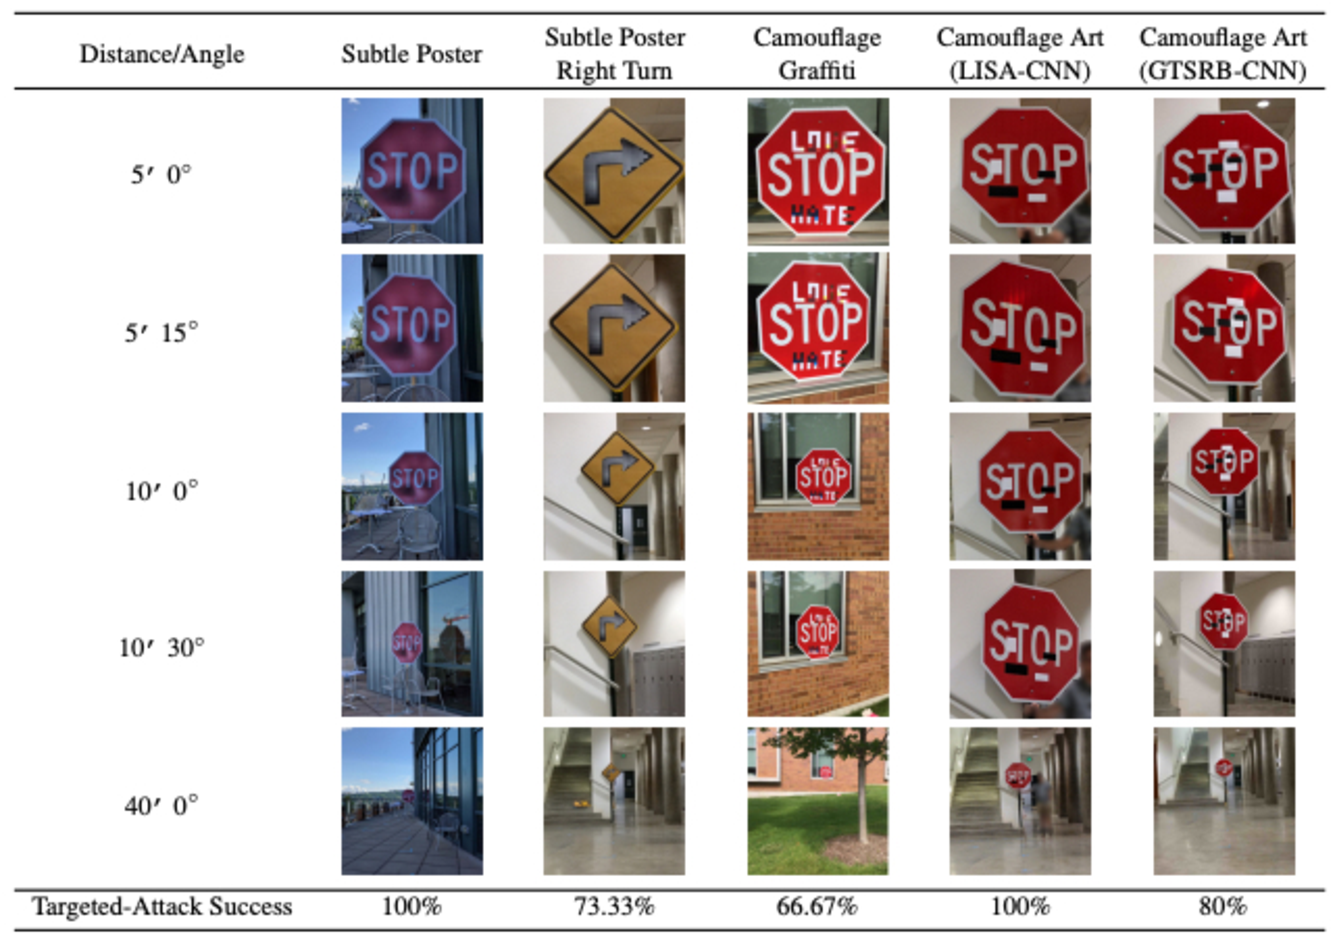
\includegraphics[width=14.0cm]{figures/robust-physical-result-image.pdf}
\end{center}
\caption{
距離と角度を変えて全 15 パターンを撮影してモデルに対する攻撃成功率を調べた結果.
画像はそのうちの 5 パターンを表示している.
Subtle Poster は摂動部分を含む画像全体を印刷したものであり, Camouflage は摂動部分のみを切り出し実際の標識に貼り付けたものになっている.
左から 2 列目と 3 列目は, mask をする部分を変更することで特定の位置にのみ摂動を加えている.
図は \cite{eykholt2018robust} より引用.
}
\label{fig:robust-physical-result-image}
\end{figure}
%

2 つめの実験の結果は図 \ref{fig:robust-physical-result-video} であり, 動画から切り出した画像に対しても摂動が有効に機能していることを示している.
標識部分を手動で crop して実験している点など実際の自動運転システムを攻撃するという観点からはまだまだ非現実的な点もあるが, digital な攻撃に比べれば現実的な physical attack の実現には大きく近づいていることが分かる.
%
\begin{figure}[htbp]
\begin{center}
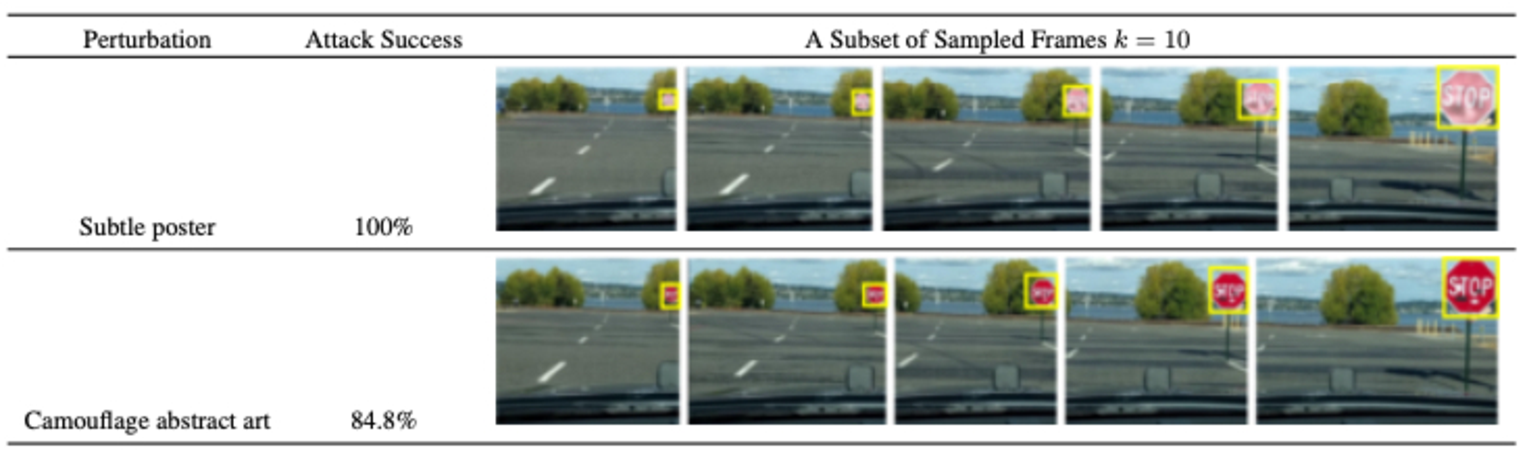
\includegraphics[width=15.0cm]{figures/robust-physical-result-video.pdf}
\end{center}
\caption{
実際に走行する車からスマートフォンで撮影した動画を 10 フレーム毎に切り出して標識部分を crop して, モデルに分類をさせて攻撃成功率を測定した結果.
図は \cite{eykholt2018robust} より引用.
}
\label{fig:robust-physical-result-video}
\end{figure}
%

この手法は検証実験のデータ量という点では不十分だが, digital な攻撃から physical な攻撃の実現可能性を高めたという点で注目に値すべきものである.
adversarial examples を作る根本的な方針自体は FGSM のようなシンプルなものからそう離れてはいないが, 距離や角度や輝度のような撮影環境が異なる場合にも攻撃成功率が高くなるように,  mask を作成して対象物のみに摂動を加えているという点が新しい.
これは以降の研究でもたびたび用いられることになる.



\subsection{One Pixel Attack for Fooling Deep Neural Networks}
\label{subsec:one-pixel}
%
\begin{table}[htbp]
\begin{center}
\begin{tabular}{|c|c|}
\hline
分類の観点 & この手法が該当するもの \\
\hline
Digital $\lor$ Physical & Digital \\
Classifier $\lor$ Detector & Classifier \\
摂動作成時に使用するデータ & 攻撃対象データ \\
摂動の加え方 & 画像全体 (ただし数ピクセルのみ) \\
知覚しづらさの定義 & 変更したピクセル数 \\
White box $\lor$ Black box & Black box \\
\hline
\multicolumn{2}{|c|}{非公式実装: \href{https://github.com/Hyperparticle/one-pixel-attack-keras}{https://github.com/Hyperparticle/one-pixel-attack-keras}} \\
\hline
\end{tabular}
\label{tb:one-pixel-summary}
\end{center}
\end{table}
%

これは \cite{su2019one} によって提案された手法であり, 差分進化アルゴリズムを用いて少数ピクセル (典型的には 1 $\sim$ 5 ピクセル) のみを変更することで誤認識させることに成功している.

この手法の特徴はモデルの勾配情報を用いない black box な攻撃であることと, 摂動として数ピクセルのみを対象としていることである.
変更されたピクセル数を知覚しづらさとして定義することができるが, これは同じ 1 ピクセルのみの変更でも人間にとって違いが明白な場合と不明瞭な場合がある.

使用しているアルゴリズムの本質的な部分は, 入力データの $i$ 成分を $x_i$ として, 世代 $g$ における値を以下のように決めることである.
%
\begin{eqnarray}
x_i (g + 1) = x_{r1} (g) + 0.5 (x_{r2} (g) - x_{r3} (g)) \ \ \text{where} \ \ r1 \neq r2 \neq r3.
\label{eq:de}
\end{eqnarray}
%
ここで, $r1, r2, r3$ は $i$ と同じ値の範囲を取る乱数である.
まず初期値としてランダムに 400 個の $x(g=0)$ を作成し, 差分進化アルゴリズム \ref{eq:de} を用いて新たに 400 個の $x(g=1)$ を作成して $x(g=0)$ と比べてモデルの softmax 値の意味で攻撃が成功に近づく方を残す.
特定のラベルに誤認識させたい場合は $y_{\text{atk-tge}}$ を設定してそれに対応する softmax 値が高くなるようにして, 特定のラベルを設定しない場合は $y_{\text{true}}$ に対応する softmax 値が小さくなるようにする.
$y_{\text{atk-tge}}$ を設定する場合は 90\% 以上になるか, 設定しない場合は 5\% 以下になるか, 世代が 100 になるまで進化を繰り返す.

kaggle CIFAR10 (\href{https://www.kaggle.com/c/cifar-10/data}{https://www.kaggle.com/c/cifar-10/data}) をデータとして用いる場合, 使用モデルは convolution のみで構成した AllConv と NIN \cite{lin2013network} と VGG16 である.
adversarial examples の作成に時間を要するため, CIFAR10 ではテストデータから 500 件ランダムにサンプリングして検証している.
ILSVRC2012 をデータとして用いる場合, 使用モデルは AlexNet である.
ILSVRC2012 ではテストデータから 105 件ランダムにサンプリングして検証している.

特徴的な結果は図 \ref{fig:one-pixel-example} のようになっており, 画像中の 1 ピクセルを変更するだけで特定のクラスに誤認識させることができていることが分かる.
%
\begin{figure}[htbp]
\begin{center}
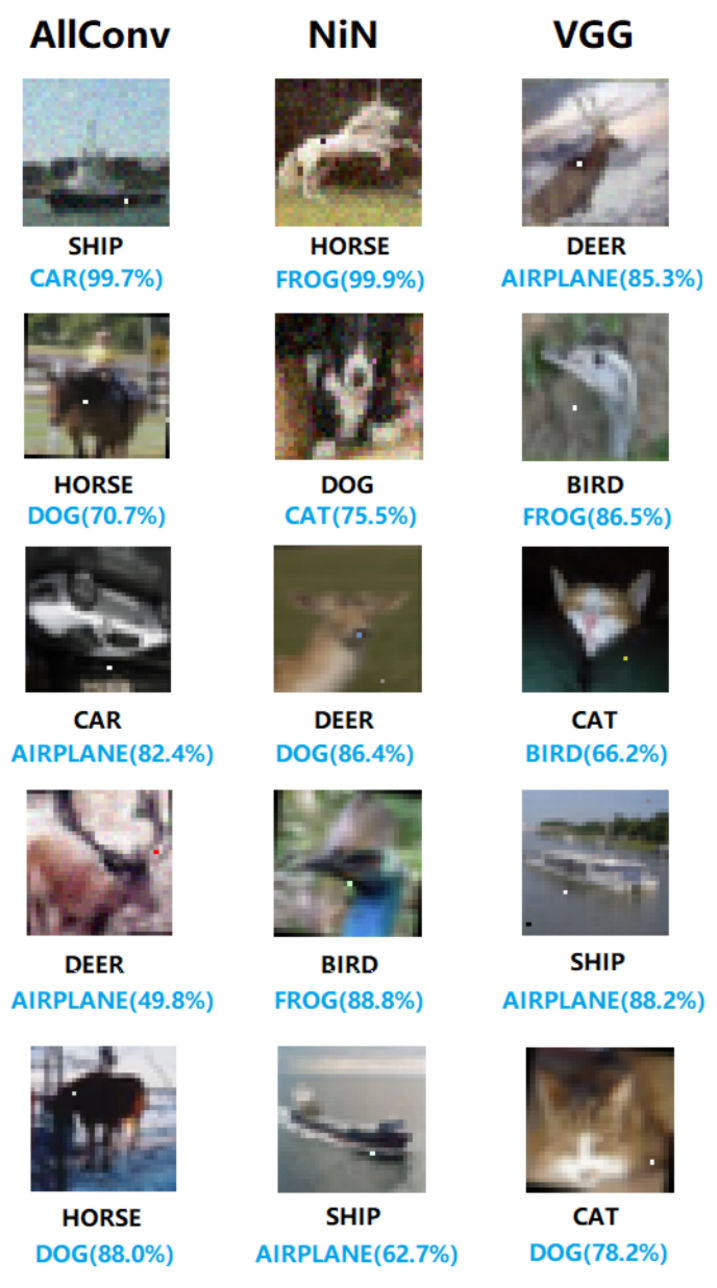
\includegraphics[width=8.0cm]{figures/one-pixel-example.pdf}
\end{center}
\caption{
kaggle CIFAR10 データに対して作成した adversarial examples の例.
黒字のクラスは $y_{\text{true}}$ で青字のクラスが $y_{\text{atk-tgt}}$ であり, どの画像も $y_{\text{atk-tgt}}$ クラスと予測されている.
図は \cite{su2019one} より引用.
}
\label{fig:one-pixel-example}
\end{figure}
%

CIFAR10 に対する adversarial examples は 1 ピクセルの変更でも人間にとって知覚しやすい.
これは画像サイズが小さいために変更箇所が顕著になるためで, ILSVRC2012 に対する adversarial examples は図 \ref{fig:one-pixel-imagenet} が示すように認識するのが難しい.
%
\begin{figure}[htbp]
\begin{center}
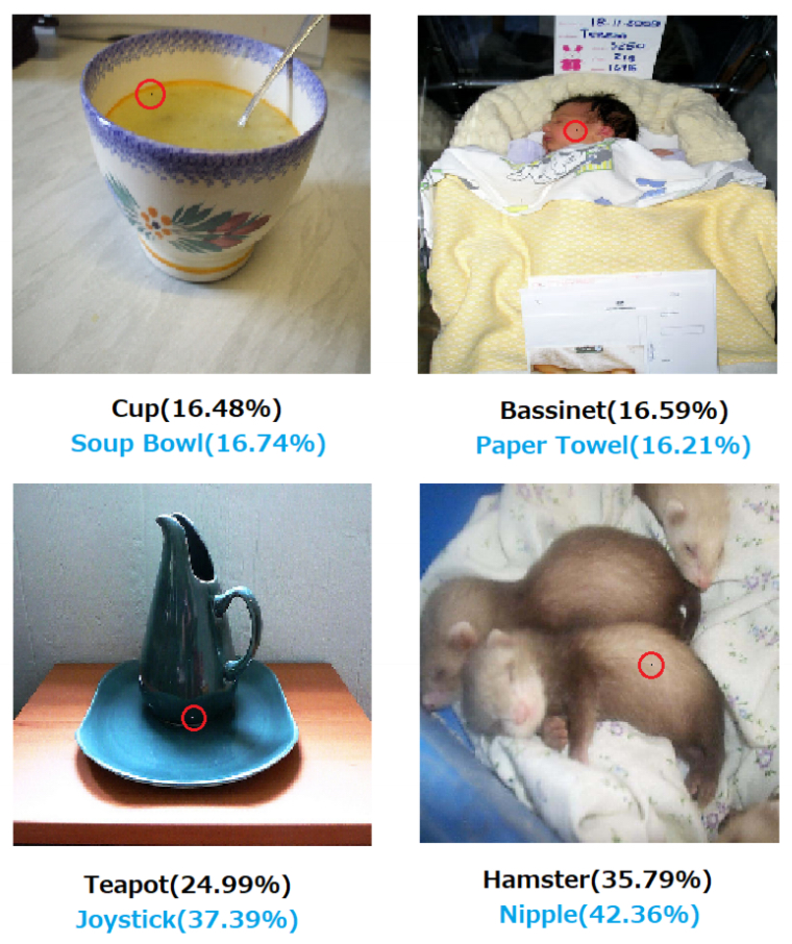
\includegraphics[width=8.0cm]{figures/one-pixel-imagenet.pdf}
\end{center}
\caption{
AlexNet モデルで ILSVRC2012 データに対して作成した adversarial examples の例.
黒字のクラスは $y_{\text{true}}$ で青字のクラスが $y_{\text{atk-tgt}}$ であり, どの画像も $y_{\text{atk-tgt}}$ クラスと予測されている.
赤い丸は変更したピクセルを視認しやすくするために後から付与した目印である.
図は \cite{su2019one} より引用.
}
\label{fig:one-pixel-imagenet}
\end{figure}
%

攻撃性能を調べた結果が図 \ref{fig:one-pixel-table} である.
Targeted ($y_{\text{atk-tgt}}$ を設定する場合) に比べると, Non-targeted ($y_{\text{atk-tgt}}$ を設定しない場合) はどのクラスに間違えさせても攻撃成功となるため誤認識率は上がっている.
ILSVRC2012 のように画像サイズが大きい場合でも成果ラベルうち 16\% を誤認識させることができている.
%
\begin{figure}[htbp]
\begin{center}
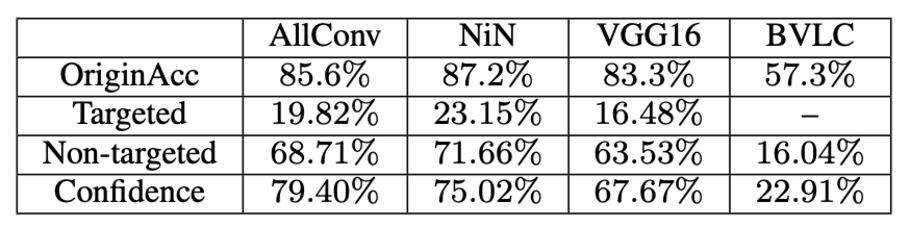
\includegraphics[width=10.0cm]{figures/one-pixel-table.pdf}
\end{center}
\caption{
1 ピクセルの変更による adversarial examples を作成して誤認識率を調べた結果.
OriginalAcc は clean データに対する正答率で, Targeted と Non-targeted は誤認識率を表している.
Confidence はモデルの softmax 値の最大の要素を平均した結果である.
モデルの BVLC は AlexNet を指している.
AllConv, NIN, VGG16 に関しては CIFAR10 を用いて, BVLC に関しては ILSVRC2012 を用いている.
Targeted の結果は正解以外の 9 クラスの結果を平均して算出しており, ILSVRC2012 の場合は計算量が多くなるため実施していない.
図は \cite{su2019one} より引用.
}
\label{fig:one-pixel-table}
\end{figure}
%

論文では変更するピクセル数を 3 ピクセルや 5 ピクセルに増やすことによる攻撃性能の向上や, 単なるランダム探索と比べて差分進化の有効性を示したりもしているが, ここでは割愛する.

この手法は摂動を加えるのが数ピクセルであっても DNN を誤認識させることができるという興味深い結果であったため注目を集めた.
攻撃成功率はそこまで高くはないが, ILSVRC2012 のように数百 $\times$ 数百ピクセルという画像においても有効であり, 人間ではほとんど気付かない adversarial examples を作成し得る.
また, DNN の予測がいかに不安定なものであるかを改めて認識させるものであった.



\subsection{Generating Natural Adversarial Examples}
\label{subsec:generating-natual}

\begin{table}[htbp]
\begin{center}
\begin{tabular}{|c|c|}
\hline
分類の観点 & この手法が該当するもの \\
\hline
Digital $\lor$ Physical & Digital \\
Classifier $\lor$ Detector & Classifier \\
摂動作成時に使用するデータ & 学習データと攻撃対象データ \\
摂動の加え方 & GANで画像を生成 \\
知覚しづらさの定義 & 潜在空間での $l_2$ \\
White box $\lor$ Black box & Black box \\
\hline
\multicolumn{2}{|c|}{公式実装: \href{https://github.com/zhengliz/natural-adversary}{https://github.com/zhengliz/natural-adversary}} \\
\hline
\end{tabular}
\label{tb:generating-natual-summary}
\end{center}
\end{table}

これは \cite{zhao2017generating} によって提案された手法であり, adversarial examples 作成の概要は図 \ref{fig:generating-natural-summary} のようになっている.
入力データ $x$ を inverter を用いて潜在空間に写し, 潜在空間で摂動を加えてそれを generator で入力データと同じ空間に写すことで $x_{\text{adv}}$ を作成する.
このとき, generator で写した $x_{\text{adv}}$ が $f_{\text{label}} (x_{\text{adv}}) \neq f_{\text{label}} (x)$ となるように要請する.
入力データの空間ではなく潜在空間での摂動を考えることで, 入力データと意味的に近いが予測結果は異なるような自然な adversarial examples が作れると期待している.
また, この手法は画像データにもテキストデータにも適用することができる.
%
\begin{figure}[htbp]
\begin{center}
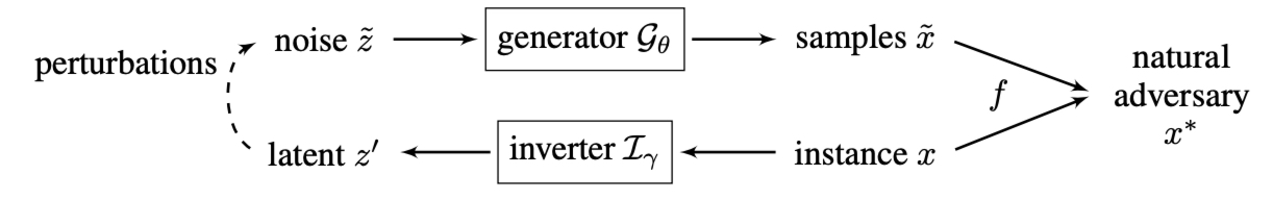
\includegraphics[width=14.0cm]{figures/generating-natural-summary.pdf}
\end{center}
\caption{
adversarial examples 作成の概要.
摂動は入力データの空間ではなく潜在空間で与える.
図は \cite{zhao2017generating} より引用.
}
\label{fig:generating-natural-summary}
\end{figure}
%

この手法は generator $\mathcal{G}_{\theta}$ と critic (discriminator) $\mathcal{C}_{\omega}$ から成る GAN の仕組みに加えて, inverter $\mathcal{I}_{\gamma}$ という入力データを潜在空間に写す三つ組から構成される.
学習の全体図は図 \ref{fig:generating-natural-training} のようになっている.
%
\begin{figure}[htbp]
\begin{center}
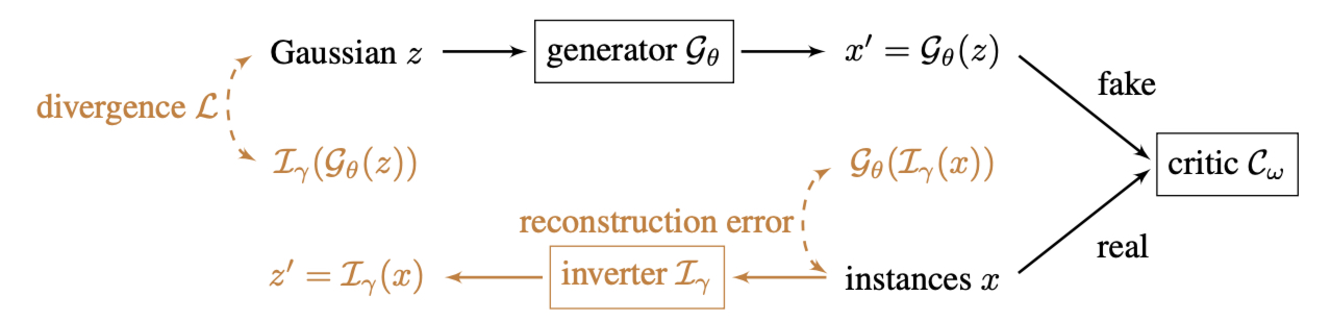
\includegraphics[width=14.0cm]{figures/generating-natural-training.pdf}
\end{center}
\caption{
generator, critic, inverter の三つ組の学習の全体図.
divergence $4\mathcal{L}$ は loss function $J$ に対応している.
図は \cite{zhao2017generating} より引用.
}
\label{fig:generating-natural-training}
\end{figure}
%
まず, generator と critic の学習は通常の GAN の枠組み通りで, Wasserstein-1 距離を用いて以下の min-max を解く.
%
\begin{eqnarray}
\min_{\theta} \max_{\omega} \left[ \mathbb{E}_{x \sim p_x (x)} \left[ \mathcal{C}_{\omega} (x) \right] - \mathbb{E}_{z \sim p_z (z)} \left[ \mathcal{C}_{\omega} (\mathcal{G}_{\theta} (z)) \right] \right].
\label{eq:gan-wasserstein}
\end{eqnarray}
%
この手法ではさらに inverter を次のように学習する.
%
\begin{eqnarray}
\min_{\gamma} \left[ \mathbb{E}_{x \sim p_x (x)} \| \mathcal{G}_{\theta} (\mathcal{I}_{\gamma} (x)) - x \| + \lambda \mathbb{E}_{z \sim p_z (z)} \left[ J(z, \mathcal{I}_{\gamma} (\mathcal{G}_{\theta} (z)) \right] \right].
\label{eq:inverter-training}
\end{eqnarray}
%
これは, 第一項は入力データを inverter で潜在空間に写してそれを generator で入力データの空間に戻した時に元の入力を再現するように要請しているもので, 第二項は潜在空間でのノイズを generator で入力データの空間に写してそれを inverter で戻したときに元のノイズを再現するように要請しているものである.
第二項は第一項の逆向きの流れを辿っているが, loss や扱うデータによって扱い方を変えている.
画像データの場合は loss function として $l_2$ ノルムを使い, $\lambda = 0.1$ としている.
学習自体は clean データのみを使用している.

学習した inverter と generator を用いて adversarial examples を作成する.
入力データ $x$ と攻撃対象のモデル $f_{\text{label}}$ があるとき, 入力データに潜在空間の $l_2$ の意味で近いが異なるラベルに予測されるような adversarial examples を作ることを目的としている.
これは以下のようにして実現される.
%
\begin{eqnarray}
x_{\text{adv}} = \mathcal{G}_{\theta} (z^*) \ \ \text{where} \ \ z^* = \argmin_{z'} \| z' - \mathcal{I}_{\gamma} (x) \| \ \text{s.t.} \ f_{\text{label}} (\mathcal{G}_{\theta} (z')) = f_{\text{label}} (x).
\label{eq:search-adversarial-example}
\end{eqnarray}
%
潜在空間でのノイズの加え方には指針がないため, 基本的にはランダム探索をする必要がある.
単に元の入力 $x$ を潜在空間に写した $z$ から近いところをランダムに探索して予測結果が変わるものを探すのは効率が悪いため, 論文では広い範囲を探索してからそれを二分探索で狭くしていくという方法を用いて 4 倍ほど高速化したと報告している.

実験としては MNIST と LSUN \cite{yu2015lsun} で実施している.
まず, MNIST で作成した adversarial examples と摂動部分を調べた例が図 \ref{fig:generating-natural-mnist} である.
FGSM で作成した摂動は画像全体に渡り, 3 という数字との関連の見えないものになっているが, 提案手法で作成した摂動は 3 という数字に合わせたものになっており, より元の入力データに意味的に近いが異なるモデル予測を導くものになっていることが見て取れる.
%
\begin{figure}[htbp]
\begin{center}
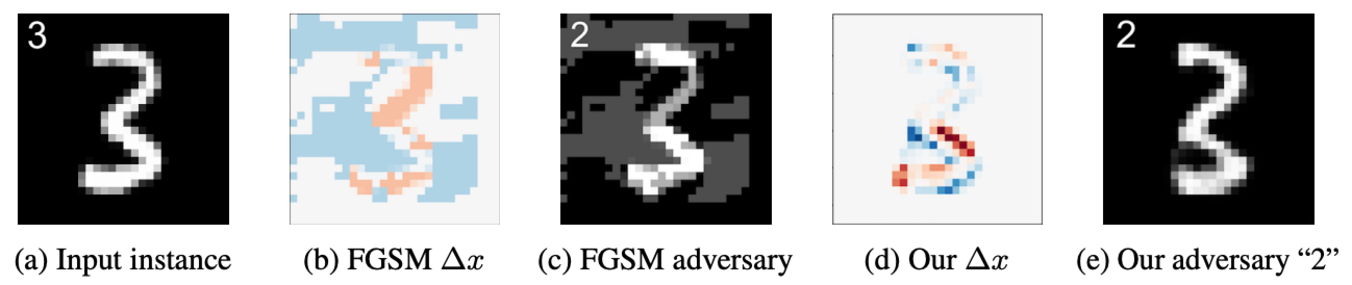
\includegraphics[width=14.0cm]{figures/generating-natural-mnist.pdf}
\end{center}
\caption{
MNIST で作成した摂動と adversarial examples の例.
$\Delta x$ は作成した摂動である.
図は \cite{zhao2017generating} より引用.
}
\label{fig:generating-natural-mnist}
\end{figure}
%

次に LSUN の結果が図 \ref{fig:generating-natural-example} である.
生成している画像なので不自然な画像にはなってしまっているが, 誤認識させたいラベルの雰囲気を似せるように変換されている様子が見て取れる.
%
\begin{figure}[htbp]
\begin{center}
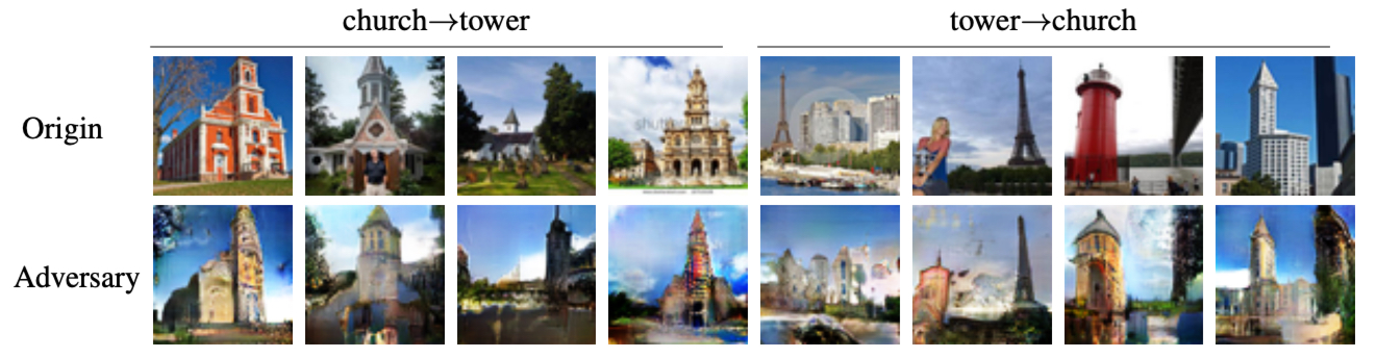
\includegraphics[width=14.0cm]{figures/generating-natural-example.pdf}
\end{center}
\caption{
LSUN で作成した adversarial examples の例.
元のラベルが {\it church} と {\it tower} のものをもう一方のものに誤認識させる adversarial examples になっている.
図は \cite{zhao2017generating} より引用.
}
\label{fig:generating-natural-example}
\end{figure}
%

どのくらいこの手法の攻撃が効率的なのかという観点で潜在空間での $z$ と $z^*$ の $l_2$ 距離の平均などを計測しているが, これらにそれほど意味は感じられないため割愛する.
また, この論文では入力データ空間での差分は気にしておらず, それは generator で生成される画像が見た目が元の入力データから離れていたとしても自然であると仮定しているためである (が, 例で見たようにこの時点での generator ではそれほど自然な画像は生成できていない).

この手法の興味深い点は入力データ空間ではなく潜在空間で摂動を加えるという点にある.
発表当時の GAN のレベルでは複雑なデータに対して十分自然な画像を生成することは難しかったが, 現在の発展に基づきより自然な画像で誤認識を引き起こすものを生成してみるのは面白いかもしれない.



\subsection{Beyond Pixel Norm-Balls: Parametric Adversaries using an Analytically Differentiable Renderer}
\label{subsec:beyond-pixel}
%
\begin{table}[htbp]
\begin{center}
\begin{tabular}{|c|c|}
\hline
分類の観点 & この手法が該当するもの \\
\hline
Digital $\lor$ Physical & Digital (防御は Physical) \\
Classifier $\lor$ Detector & Classifier \\
摂動作成時に使用するデータ & 3D object データ \\
摂動の加え方 & 対象物のみ \\
知覚しづらさの定義 & 色味が変わるなどの定性的評価 \\
White box $\lor$ Black box & White box \\
\hline
\multicolumn{2}{|c|}{実装なし (著者にメールしたが返信なし)} \\
\hline
\end{tabular}
\label{tb:beyond-pixel-summary}
\end{center}
\end{table}
%

これは \cite{liu2018beyond} によって提案された手法であり, 3D object データと微分可能レンダラーを用いて対象物の形状に沿った摂動を加えることで実現する色味や形状の変化で誤認識を引き起こす.

この手法を理解するためにはレンダリングの基礎知識が必要となるが, ここでは既知のものとして割愛する\footnote{
概念のみを述べておくと, レンダリングとは光学系をシミュレートして 3D 情報から 2D 画像を生成することである.
原論文の Appendix B に簡単な解説が書いてあるので, 興味があれば読んでみるのがよいだろう.
微分可能レンダラーはレンダラー部分も DNN で表現することで微分可能な構造を提供し, 誤差の伝播などを扱いやすくしたレンダラーである.
}.
レンダラーと 3D オブジェクトの情報があれば, まず対象となるオブジェクトに対してのみ適用される摂動を作成することができる.
そしてそれが 2D 画像に投影することができるため, 対象オブジェクトのみに摂動が加えられた adversarial examples が作成できる.
この論文では対象オブジェクトに加える摂動として lighting ($U$) と geometry ($V$) なるものを考案している.
例としては図 \ref{fig:beyond-pixel-example} のようなものとなる.
提案手法が物体形状に沿った自然な摂動になっていることが見て取れる.
%
\begin{figure}[htbp]
\begin{center}
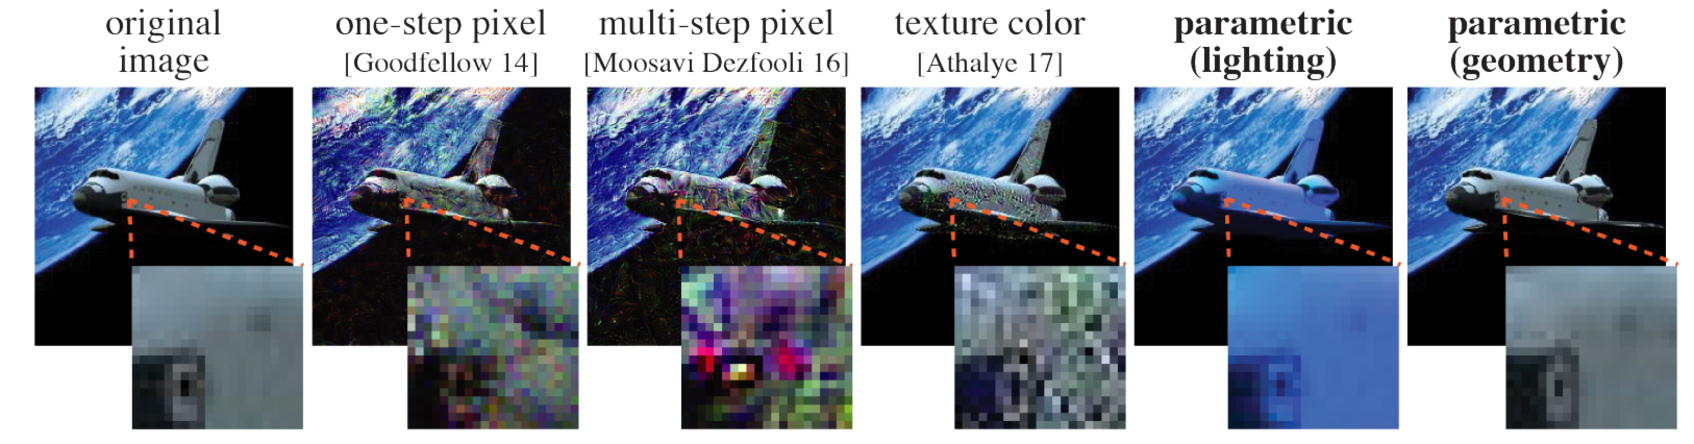
\includegraphics[width=14.0cm]{figures/beyond-pixel-example.pdf}
\end{center}
\caption{
提案手法による摂動の例.
まず, 各画像は 2D の背景画像の上に 3D の飛行機のオブジェクトをレンダリングして 2D 画像を作成している.
攻撃方法の左 2 つは作成した 2D 画像に対して摂動を加えるため摂動は画像全体に広がっている.
texture color はオブジェクトのみに摂動を加える先行研究で, 3D オブジェクトに対して摂動を作成してそれを 2D にレンダリングしているので飛行機のみに摂動が加えられているが, 不自然な摂動となっていて人間が気付きやすい.
右 2 つの提案手法も摂動を 3D オブジェクトに対して作成してからレンダリングしているが, 色味やわずかな形状を変えるのみで自然な摂動になっている.
図は \cite{liu2018beyond} より引用.
}
\label{fig:beyond-pixel-example}
\end{figure}
%

微分可能レンダラー \cite{kato2018neural} を用いることで, 2D 画像に対する loss を逆伝播して 3D オブジェクトに反映させることが可能となる.
つまり, 3D オブジェクトからスタートして, それを微分可能レンダラーに通して 2D 画像を作成し, 予測モデルでその 2D 画像に対する loss を計算する, を逆向きに辿っていって予測モデルが誤認識する摂動を 3D オブジェクトに加えることができる.
摂動として自然なものを作成するため, この論文では 3D オブジェクトのパラメタを用いて lighting ($U$) と geometry ($V$) を定義する.
これらは低次の球面調和関数の係数や 3D オブジェクトを三角分割した際の法線や頂点などで記述されるが, ここでは詳細を割愛する.
微分可能レンダラーを介して 2D 画像 $I$ を $I(U, V)$ と書くことができるため (微分可能レンダラーのパラメタは陽には書いていない), 以下のように loss を微分した量が計算できれば勾配法で摂動が作成できる.
%
\begin{eqnarray}
\frac{\partial J}{\partial U} &=& \frac{\partial J}{\partial I} \frac{\partial I}{\partial U}.\\
\frac{\partial J}{\partial V} &=& \frac{\partial J}{\partial I} \frac{\partial I}{\partial V}.
\label{eq:beyond-pixel-diff}
\end{eqnarray}
%
それぞれ右辺の第一項は loss function を 2D 画像で微分しているのみなので特に難しいところはない.
第二項は 2D の画像を 3D オブジェクトのパラメタで微分するため, 微分可能レンダラーを介して計算される量である.

具体的な表式を割愛すれば, 手法としては以上である.
lighting を変えた誤認識させる例は図 \ref{fig:beyond-pixel-lighting} である.
対象物の色味が変わっているだけなので, 摂動としては不自然さは少ない (3D オブジェクトをレンダリングして作成しているので背景画像とのミスマッチ感はある).
%
\begin{figure}[htbp]
\begin{center}
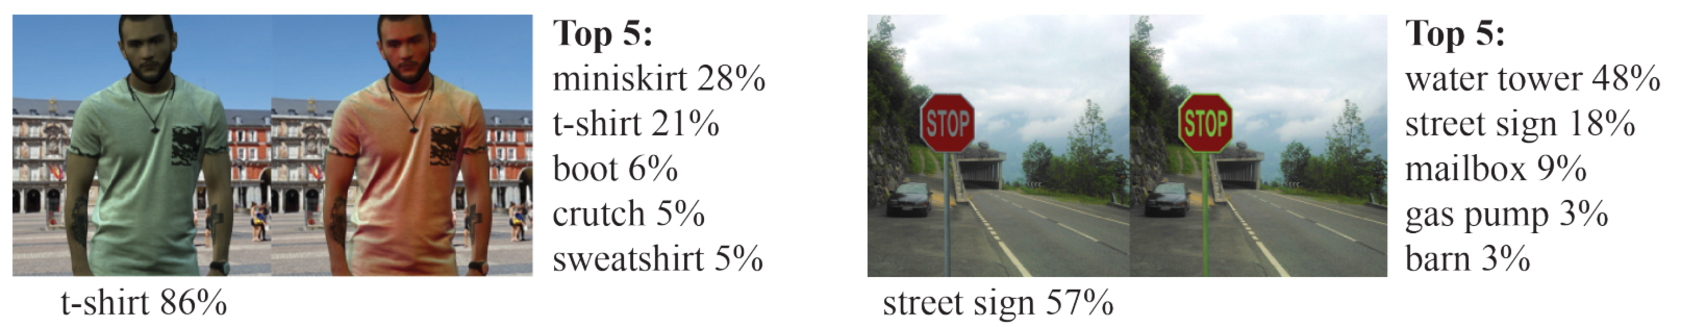
\includegraphics[width=14.0cm]{figures/beyond-pixel-lighting.pdf}
\end{center}
\caption{
lighting を変えて作成した adversarial examples の例.
背景の 2D 画像に lighting を変えた 3D オブジェクトをレンダリングして最終的な 2D 画像を作成している.
モデルによる予測は ILSVRC2012 で pre-train された ResNet-101 で実施している.
図は \cite{liu2018beyond} より引用.
}
\label{fig:beyond-pixel-lighting}
\end{figure}
%

3D オブジェクトに対する手法であるため, 様々に角度を変えても同じように誤認識させる摂動を作成することもできる.
それを示したのが図 \ref{fig:beyond-pixel-diff-angle} であり, 異なる角度に対してもモデルが同様に誤認識している様子が見て取れる.
%
\begin{figure}[htbp]
\begin{center}
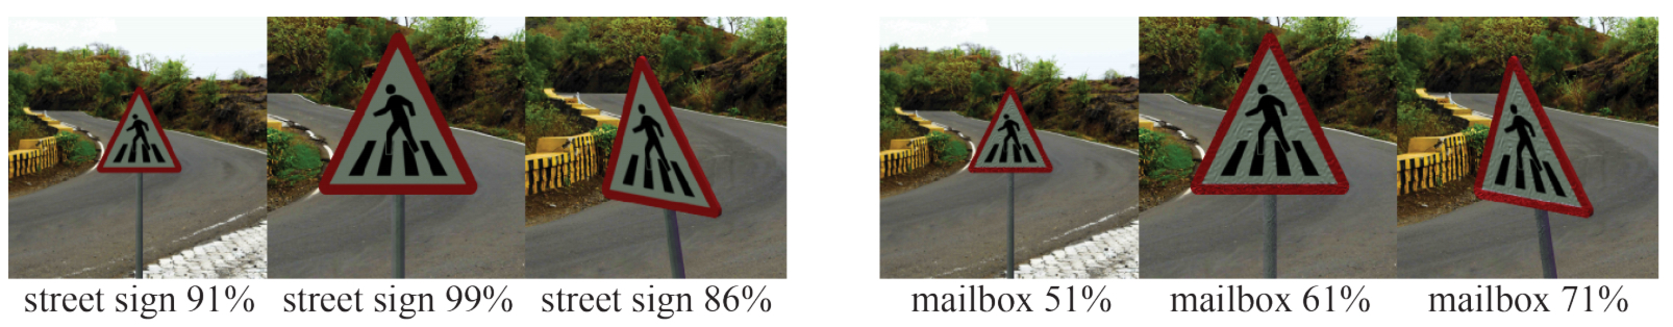
\includegraphics[width=14.0cm]{figures/beyond-pixel-diff-angle.pdf}
\end{center}
\caption{
角度を変えても同様に誤認識をさせることに成功している例.
摂動は geometry に対して作成している.
背景の 2D 画像に lighting を変えた 3D オブジェクトをレンダリングして最終的な 2D 画像を作成している.
モデルによる予測は ILSVRC2012 で pre-train された ResNet-101 で実施している.
図は \cite{liu2018beyond} より引用.
}
\label{fig:beyond-pixel-diff-angle}
\end{figure}
%

提案手法による摂動は対象物のみに加える摂動で対象物の光学的・幾何学的変換に基づくものであるため, より対象物そのものの性質を捉えたもので adversarial examples として transferability も高い.
ResNet で作成した 5,000 枚の adversarial examples を他のモデルで検証した結果が図 \ref{fig:beyond-pixel-transferability} で, 多くのモデルが高い確率で誤認識している.
%
\begin{figure}[htbp]
\begin{center}
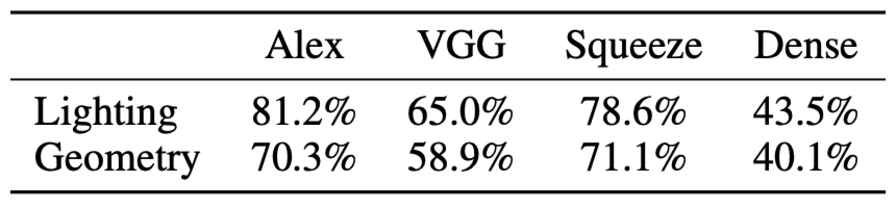
\includegraphics[width=8.0cm]{figures/beyond-pixel-transferability.pdf}
\end{center}
\caption{
ResNet で作成した 5,000 枚の adversarial examples に対する他のモデルの誤認識率 (1 - 正答率).
モデルは AlexNet, VGG, SqueezeNet \cite{iandola2016squeezenet}, DenseNet \cite{huang2017densely} を用いている.
図は \cite{liu2018beyond} より引用.
}
\label{fig:beyond-pixel-transferability}
\end{figure}
%

この手法は微分可能レンダラーを用いて 3D オブジェクトに対して摂動を作成してそれを 2D に写すという点が興味深い.
より対象物に特化した摂動を作成することが可能になっている.
必要となる道具が多いのと 3D オブジェクトデータも必要になる手法ではあるが, \cite{athalye2017synthesizing} のように 3D プリンターで作成した adversarial examples も登場しているため, 一つの面白い方向性だろう.



\subsection{On the Structural Sensitivity of Deep Convolutional Networks to the Directions of Fourier Basis Functions}
\label{subsec:on-the}
%
\begin{table}[htbp]
\begin{center}
\begin{tabular}{|c|c|}
\hline
分類の観点 & この手法が該当するもの \\
\hline
Digital $\lor$ Physical & Digital \\
Classifier $\lor$ Detector & Classifier \\
摂動作成時に使用するデータ & 学習データ \\
摂動の加え方 & 画像全体 \\
知覚しづらさの定義 & $l_{\infty}$ \\
White box $\lor$ Black box & Black box  (出力ラベルのみ) \\
\hline
\multicolumn{2}{|c|}{実装なし} \\
\hline
\end{tabular}
\label{tb:on-the-summary}
\end{center}
\end{table}
%

これは \cite{tsuzuku2019structural} によって提案された手法であり, 周波数領域でフーリエ基底を用いてデータに依らない adversarial examples を作成する.
DNN は adversarial examples に対して線形分類器に近い振る舞いをするという経験的事実と, CNN が周波数領域で特徴量を学習しているという経験的事実を合わせて, 周波数領域で摂動を構成することでデータに依らずに様々な CNN に対して有効な adversarial examples の作成を実現している. 
adversarial examples 作成時にモデルの出力ラベルのみを用いる真の black box attack となっている点も特徴である.

道具としてフーリエ基底や離散フーリエ変換が必要となるため, 簡単に復習する.
虚数の N 乗根を $s_N = \exp (2 \pi i / N)$ として, $s_N^{u,v} = s_N^u s_N^v \in \mathcal{C}^{N \times N}$ とする.
これを用いて以下の $N \times N$ 行列を定義する.
%
\begin{eqnarray}
(F_N)_{u,v} = \frac{1}{\sqrt{N}} s_N^{u, v}.
\label{eq:on-the-matrix}
\end{eqnarray}
%
座標領域から波数領域への離散フーリエ変換は以下のように書ける.
%
\begin{eqnarray}
S(x)_{u,v} = \sum_{m=0}^{N-1} \sum_{n=0}^{N-1} x_{m,n} \exp (- 2 \pi i (u m + v n) / N)
\label{eq:on-the-dft}
\end{eqnarray}
%
これらは単なる定義である.
二次元 $N \times N$ を考えているのは画像が二次元空間 (height, width) であることに対応している (チャンネルの次元もあるがこれらは波数を求める対象ではない).
また, 導入した $s^{u,v}$ の添字は (height, width) の波数のモードと対応していて, これらの値が大きいほど波数が大きなモードとなっていることが分かる.

導入した $F_N$ を用いた $Q_N = \frac{1}{N} F_N \otimes F_N$ ($\otimes$ はクロネッカー積) が解析において重要な量となる.
これがなぜ重要なのかを詳しく知りたい場合は \cite{sedghi2018singular} も併せて読んでもらうとして, ここでは概略だけを述べる.
重要な点はチャンネル数が 1 の 2d-convolution の padding を wrap around\footnote{
各エッジでトーラス状につながるように padding するもの.
解析のしやすさのために用いている方法で実際にはあまり用いられることはない.
}
にする場合, doubly block circulant matrix $A$ を用いて 2d-convolution の演算が $\text{vec} (x_{\text{next}}) = A \cdot \text{vec} (x)$ のように書けるという点である.
詳細な定義は文献を追ってもらうとして, wrap around のような周期性がある padding であれば数学的には特徴的な行列で表現できることは想像に難くない.
そして, この 2d-convolution の情報を持つ行列 $A$ の固有値や固有ベクトルと深く関わっているのが $Q_N = \frac{1}{N} F_N \otimes F_N$ なのである.
具体的には, 例えば $A$ の固有ベクトルは $Q_N$ の列であることが示されている.

この事実を受け入れると, $Q_N$ がユニタリであること (これは定義より自明) から $A$ は複素対角行列 $D$ を用いて $A = Q_N D Q_N^{\dagger}$ ($Q_N^{\dagger}$ は $Q_N$ のエルミート共役) と分解できる.
これは左から $Q_N^{\dagger}$, 右から $Q_N$ を掛けることで簡単に固有値が求められることを意味する.
したがって, convolution の固有値や固有ベクトルが簡単に求まるため, 特定のモードの固有ベクトルだけを取り出して摂動を作成するということが実現できる.
そのような摂動が有効かどうかはここでの数学的な議論とは別物であるが, それを期待するには十分な経験的知識があり, 試してみたら上手く機能したというストーリーになっている.

ここでの議論はチャンネル数が 1 で convolution を 1 回だけ適用してかつ線形な activation のみに有効なものであるが, 論文ではチャンネル数を増やしたり convolution を stack したり skip connection を加えても同様の議論が成り立つことを証明している.
非線形な activation を考えると数学的な保証がなくなってしまうが, ReLU のように線形な activation からそう遠く離れてない場合はある程度上手くいくことが期待でき, それは実験的にも示される.

具体的に adversarial examples を作成するアルゴリズムは次のようになる.
$(F_N)_u$ を $u$ 番目の行のベクトルとして, ある入力画像 $x$ とアルゴリズム \ref{alg:on-the-single-fourier-attack} で作成した $x_{\text{adv}}$ で予測ラベルが異なるような波数モード $u, v$ を brute force で探す.
学習データ全体に対して誤認識率が最も高くなる $u, v$ の組を探しており, 2 つの離散的な変数であるため力技で解くことができる.
%
\begin{algorithm}
\caption{Single Fourier attack のアルゴリズム}
\label{alg:on-the-single-fourier-attack}
\begin{algorithmic}[1]
    \State Input: 波数モード $u, v$, 摂動の大きさ $\epsilon$.
    \State Output: adversarial examples $x_{\text{adv}}$.
	\State adversarial examples を初期化: $x_{\text{adv}} \leftarrow x$.
	\For {各チャンネル $c$}
	\State $x_{\text{adv}} \leftarrow x_{\text{adv}} + \epsilon ( (1 + u) (F_N)_u \otimes (F_N)_v + (1 - u) (F_N)_{N - u} \otimes (F_N)_{N - v} )$.
	\State $x_{\text{adv}} \leftarrow \text{clip} (x_{\text{adv}},0,1)$.
	\EndFor
\end{algorithmic} 
\end{algorithm}
%

実験はデータとしては MNIST, fashion MNIST, SVHN, CIFAR10, CIFAR100 を用いている.
モデルは LeNet, VGG, WideResNet \cite{zagoruyko2016wide}, DenseNet を用いており, 理論解析時に要請した wrap around の padding や線形な activation は用いていない (それでも上手くいくと期待している).
画像を扱うため座標領域では実数値を取る必要があるため, $S(x)_{u,v} = S(x)^{\dagger}_{N - u, N - v}$ を満たすものだけが許容される.
この条件式は式 \ref{eq:on-the-dft} の両辺のエルミート共役を取り $x_{m,n}$ が実数値であることを要請すれば導出できる.
このような条件を満たす各 $u, v$ に関してランダムにミニバッチを選んで誤認識率を計算したものが図 \ref{fig:on-the-uvplane} である.
これはあらゆる場合でこの手法が有効であるわけでないことを示しているが, データやモデルによってこれだけ振る舞いが変わるという点は興味深い.
また, 例えば SVHN では低波数成分が強く効いていることが分かるが, CIFAR では高波数成分が効いていることが分かり, 単純に低波数成分が摂動にとって支配的でないことが示されている.
%
\begin{figure}[htbp]
\begin{center}
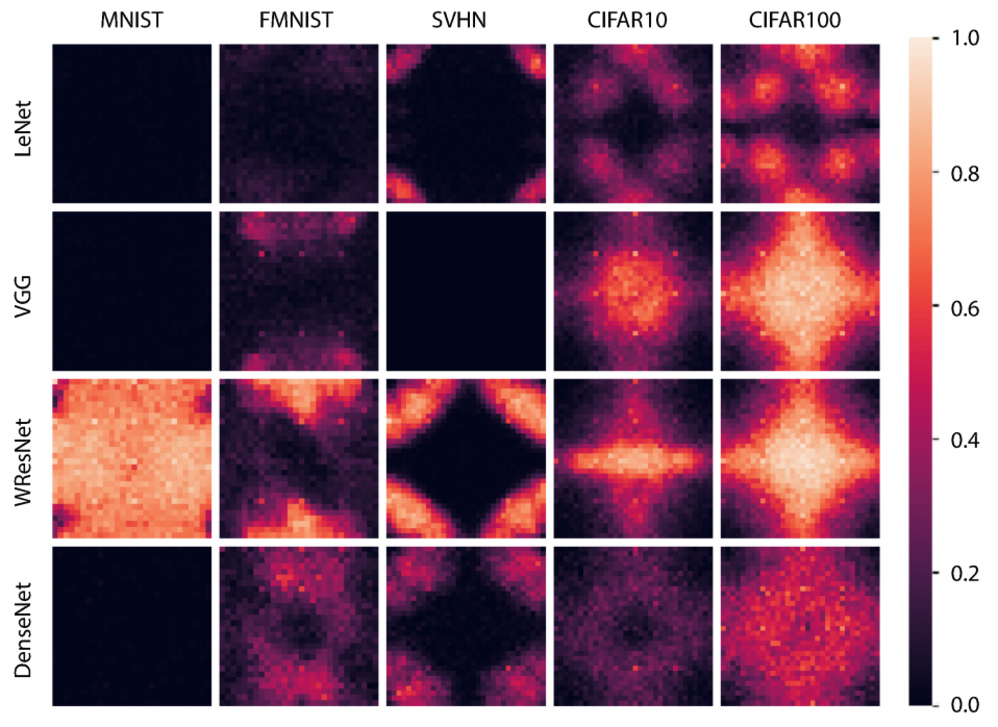
\includegraphics[width=12.0cm]{figures/on-the-uvplane.pdf}
\end{center}
\caption{
各データセット, 各モデルでの誤認識率 (1 - 正答率) を $(u, v)$ 平面でプロット結果.
色が白いところが誤認識率が高い領域である.
四隅が低波数領域で中心が高波数領域であり, これは離散フーリエ変換を考えれば $2 \pi$ が周期であるため, 例えば $u = v = N - 1$ の場合 exp の部分が $\exp (- 2 \pi i (m + n) / N)$ になり $u = v = 1$ と同じなることから理解できる.
図は \cite{tsuzuku2019structural} より引用.
}
\label{fig:on-the-uvplane}
\end{figure}
%

データセット全体に対する誤認識率を定量的に調べた結果が図 \ref{fig:on-the-fool-ratio} である.
シンプルな摂動でありながら大きく効果を発揮しているものが多い一方で, 先ほど見たように同じモデルでもデータによって全く摂動が効かないものも存在する.
また, 単純なノイズによっても WideResNet の誤認識が高くなったりもしていてモデルの構造依存性が大きいことが伺える.
%
\begin{figure}[htbp]
\begin{center}
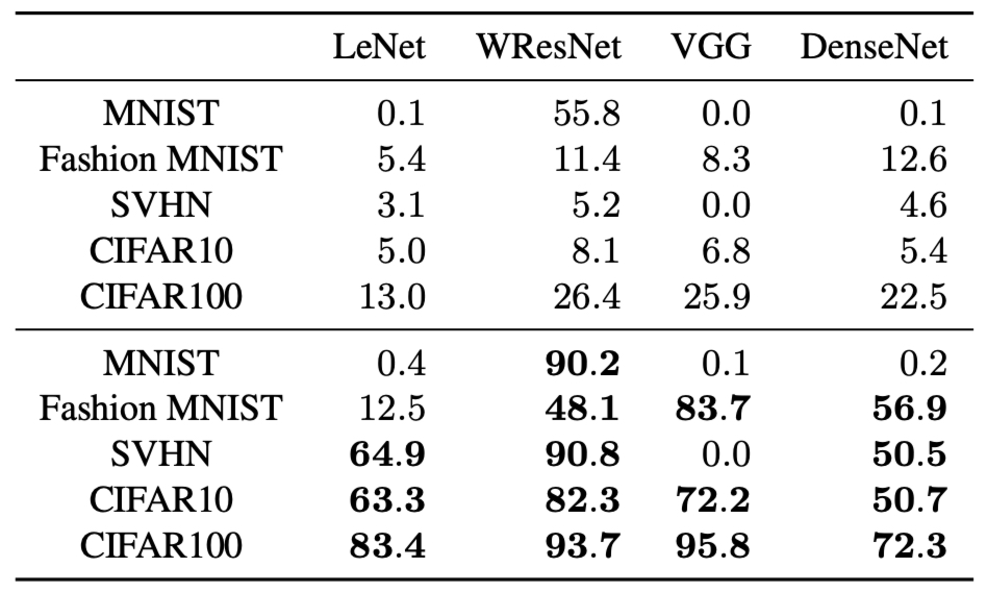
\includegraphics[width=10.0cm]{figures/on-the-fool-ratio.pdf}
\end{center}
\caption{
各データセットに対する各モデルの誤認識率 (1 - 正答率).
上段はデータにランダムなノイズを加えた結果で, 下段は Single Fourier Attack で作成した adversarial examples の結果.
図は \cite{tsuzuku2019structural} より引用.
}
\label{fig:on-the-fool-ratio}
\end{figure}
%

従来手法で作成し摂動を波数領域で調べるとどうなるのかは気になるところであるが, FGSM で作成した摂動を波数領域で調べた結果が図 \ref{fig:on-the-fgsm} である.
これは図 \ref{fig:on-the-uvplane} とは異なり誤認識率を表しているわけではなく, 作成した摂動がどの成分が大きいかを調べたものになっている.
具体的には FGSM で作成した摂動は各波数モードの線形和になっているため, 各モードに対応するベクトルの絶対値の平均を取っている.
波数で特徴付けられる摂動を作成していることが見て取れて, Single Fourier Attack の結果と同様に CIFAR では高波数モードも効いていることが分かる.
ただし, MLP のような単純なモデルではどのデータでも低波数モードのみが効いていることが分かり, シンプルな CNN では高波数成分を取り除くように重みが学習されて低波数成分が支配的であるということの一定の証拠となっている.
また, 例えば MNIST-VGG の組み合わせのように Single Fourier Attack では誤認識が確認できなかったものでも複数成分の重ね合わせをすれば誤認識させることができる.
これはフーリエ基底の一部だけで摂動を構築することの限界を示している.
%
\begin{figure}[htbp]
\begin{center}
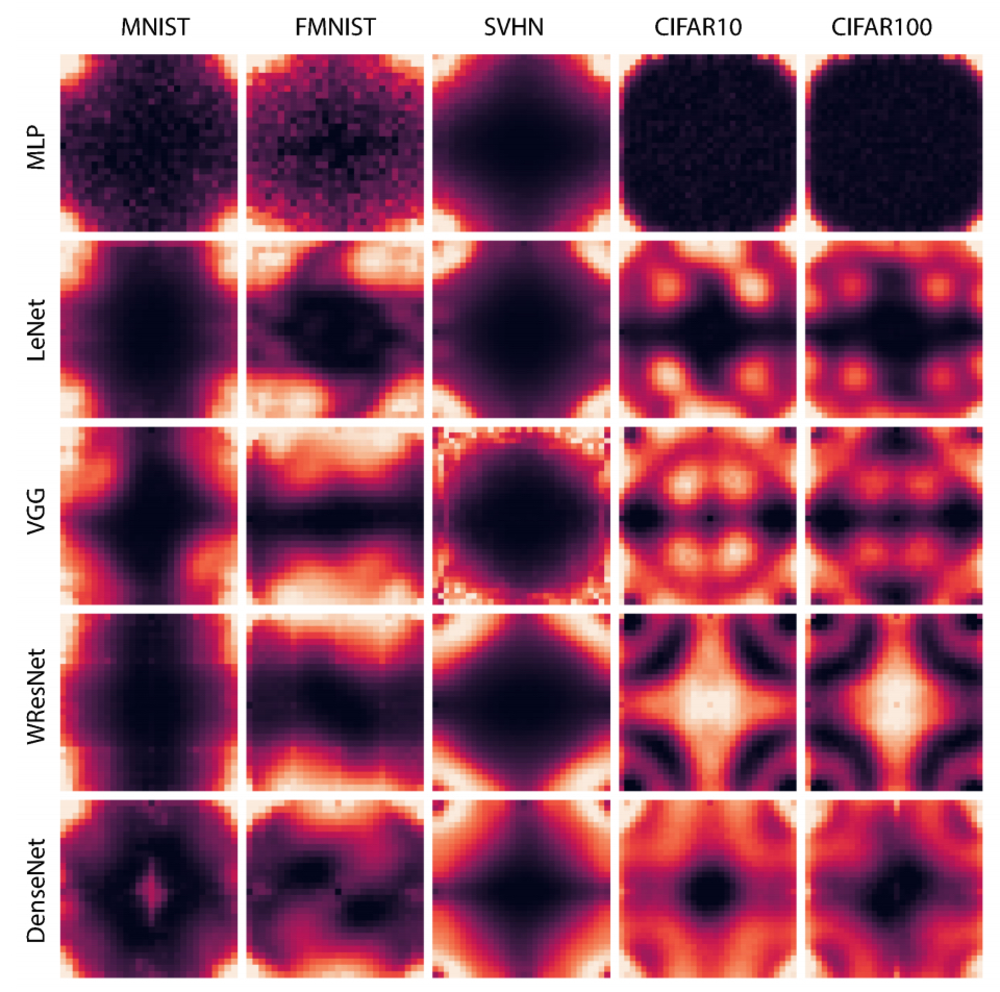
\includegraphics[width=10.0cm]{figures/on-the-fgsm.pdf}
\end{center}
\caption{
FGSM で作成した摂動の波数領域での大きさを調べたもの.
FGSM で作成した摂動は各波数モードの線形和であるため, 各モードに対応するベクトルの絶対値の平均を計算してプロットしている.
白色に近いほど値が大きい.
図は \cite{tsuzuku2019structural} より引用.
}
\label{fig:on-the-fgsm}
\end{figure}
%

この手法は CNN の固有値や固有ベクトルの解析と adversarial examples を組み合わせた点が興味深い.
理論的解析は padding として wrap around と線形な activation に限るものだが, 実際のモデルはそこから大きく外れるものではないので実験的にも作成した adversarial examples がうまく機能している.
データやモデル依存性が大きいため, このような方向性の議論を深めることでデータやモデルの特徴付けや分類が可能となるかもしれない.



\subsection{Adversarial camera stickers: A physical camera-based attack on deep learning systems}
\label{subsec:advdersarial-camera}
%
\begin{table}[htbp]
\begin{center}
\begin{tabular}{|c|c|}
\hline
分類の観点 & この手法が該当するもの \\
\hline
Digital $\lor$ Physical & Physical \\
Classifier $\lor$ Detector & Classifier \\
摂動作成時に使用するデータ & 攻撃対象データ \\
White box $\lor$ Black box & White box \\
摂動の加え方 & 画像全体 \\
知覚しづらさの定義 & ヒューリスティック \\
\hline
\multicolumn{2}{|c|}{非公式実装: \href{https://github.com/yoheikikuta/adversarial-camera-stickers}{https://github.com/yoheikikuta/adversarial-camera-stickers}} \\
\hline
\end{tabular}
\label{tb:advdersarial-camera-summary}
\end{center}
\end{table}
%

これは \cite{li2019adversarial} によって提案された手法であり, 作成した摂動をシールとして印刷してカメラのレンズに貼り付けることで攻撃対象の予測モデルの誤認識を引き起こす手法である.
従来手法が物体に摂動を加えることを考えていたのとは対照的に, カメラと物体間の光学的な path の間に操作を加えるという試みである.

摂動はカメラのレンズにシールを貼るだけで physical な環境で有効であるようなものにしたい.
少しずれたりしただけで効果が発揮されないような摂動では目的を達成できないため, あまり細かい摂動ではなくてぼやっとした摂動が適していると考えられ, この論文では色付き半透明の丸模様を複数個作成するという戦略を採用している.
具体的な数式は以下のようになる.
%
\begin{eqnarray}
(x_{\text{adv}})_{i,j} &=& (1 - \alpha_{i,j}) \cdot x_{i,j} + \alpha_{i,j} \cdot \gamma.
\label{eq:adversarial-camera-pi} \\
\alpha &=& \alpha_{\text{max}} \cdot \exp (- d^{\beta} (i,j)).
\label{eq:adversarial-camera-alpha} \\
d (i,j) &=& \frac{(i - i^{(\text{center})})^2 + (j - j^{(\text{center})})^2}{r^2}.
\label{eq:adversarial-camera-d}
\end{eqnarray}
%
ここで, $(i,j)$ は画像の二次元座標で, $\gamma \in [0, 1]^3$ で丸模様の色である.
この $x_{\text{adv}}$ ある中心 $(i^{(\text{center})}, j^{(\text{center})})$ から離れるほど指数的に薄くなる丸模様を元画像とアルファブレンディングしたものである.
この数式で表現される丸模様は一つだけだが, これを複数回適用することで実際の摂動を作成する.
あるクラス $y^{*}$ の画像 $M$ 個をまとめて $y_{\text{atk-tgt}}$ に間違えさせるという問題設定を考えていて, loss function は以下のように構成する.
%
\begin{eqnarray}
\sum_{m = 1}^{M} \left(- J(f, x_{\text{adv}}, y^*) + J(f, x_{\text{adv}}, y_{\text{atk-tgt}}) \right).
\label{eq:adversarial-camera-loss}
\end{eqnarray}
%

あとは式 \ref{eq:adversarial-camera-pi},\ref{eq:adversarial-camera-alpha},\ref{eq:adversarial-camera-d} で導入された各パラメタと丸模様の数に関してこの loss function が小さくなるように最適化して得られた結果をシールとして印刷すればよいが, パラメタが多いため最適化は容易ではない.
ヒューリスティックや予備実験によって, 丸模様の数を 10 個に固定して, $r, \alpha_{\text{max}}, \beta$ も固定し, $\gamma$ は 10 組 (その集合を $\Gamma$ とする) に限定した上で $\gamma$ とそれぞれの丸模様の中心位置について最適化を実施するという簡単化をしている.
この簡単化はかなり大変な作業で, まず物理的に実現可能, 知覚もしにくく, モデルを誤認識させることができるようなシールをヒューリスティックに作成する\footnote{
この辺りの詳細は書いてなく, 著者に聞いても詳しくは教えてくれなかったが大変だったと語っていた.
}.
このヒューリスティックに作成した摂動を再現するようなパラメタを SSIM \cite{wang2004image} を最大化するという条件で求めるというアプローチになっている.
固定したパラメタはこのようにして求めている.
残りの $\gamma$ とそれぞれの丸模様の中心位置の最適化はアルゴリズム \ref{alg:adversarial-camera-alg} で求める.
$\gamma$ は離散集合から選択するため勾配法が使えないので, まずは丸模様の中心位置も $45 \times 45$ のグリッドに離散化した状況下 ($\mathcal{C}$ と書く) での greedy な最適化を実施する.
$\gamma$ の値と大体の丸模様の中心位置が定まったら, 丸模様の中心位置は連続量に戻して勾配法で細かい調整をするという手順となる.
%
\begin{algorithm}
\caption{$\gamma$ と丸模様の中心位置を定めるアルゴリズム}
\label{alg:adversarial-camera-alg}
\begin{algorithmic}[1]
    \State Input: 丸模様の数 $K$, 攻撃対象のクラス $y^*$, ターゲットクラス $y_{\text{atk-tgt}}$, $y^*$ に属する画像 $x^{(1)}, \dots, x^{(M)}$.
    \State Output: 摂動を作成するための $\gamma_k$ と $(i^{(\text{center})}_k, j^{(\text{center})}_k)$.
	\State 摂動を初期化: $(i^{(\text{center})}_k, j^{(\text{center})}_k) \leftarrow \text{some values}$.
	\Repeat
	\For {各$k \in K$}
	\For {$(i^{(\text{center})}_k, j^{(\text{center})}_k), \gamma_k \in \mathcal{C} \times \Gamma$}
	\State 式 \ref{eq:adversarial-camera-loss} を評価.
	\EndFor
	\State loss が最小になる $(i^{(\text{center})}_k, j^{(\text{center})}_k), \gamma_k$ を選ぶ.
	\EndFor
	\Until {loss が収束するまで}
	\State
	\Repeat
	\For {$k \in K$}
	\State $(i^{(\text{center})}_k, j^{(\text{center})}_k)$ を式 \ref{eq:adversarial-camera-loss} の勾配を計算して勾配法で更新.
	\EndFor
	\Until {loss が収束するまで}
\end{algorithmic} 
\end{algorithm} 
%

最終的に作成した摂動とそれをカメラのレンズに貼って撮影した画像の例が図 \ref{fig:adversarial-camera-example} である.
どちらも誤認識させることができた画像を集めており, 様々な撮影条件において誤認識させることができていることに加え, 撮影された画像は少し汚れのように色がついているのが認識される程度である.
%
\begin{figure}[htbp]
\begin{center}
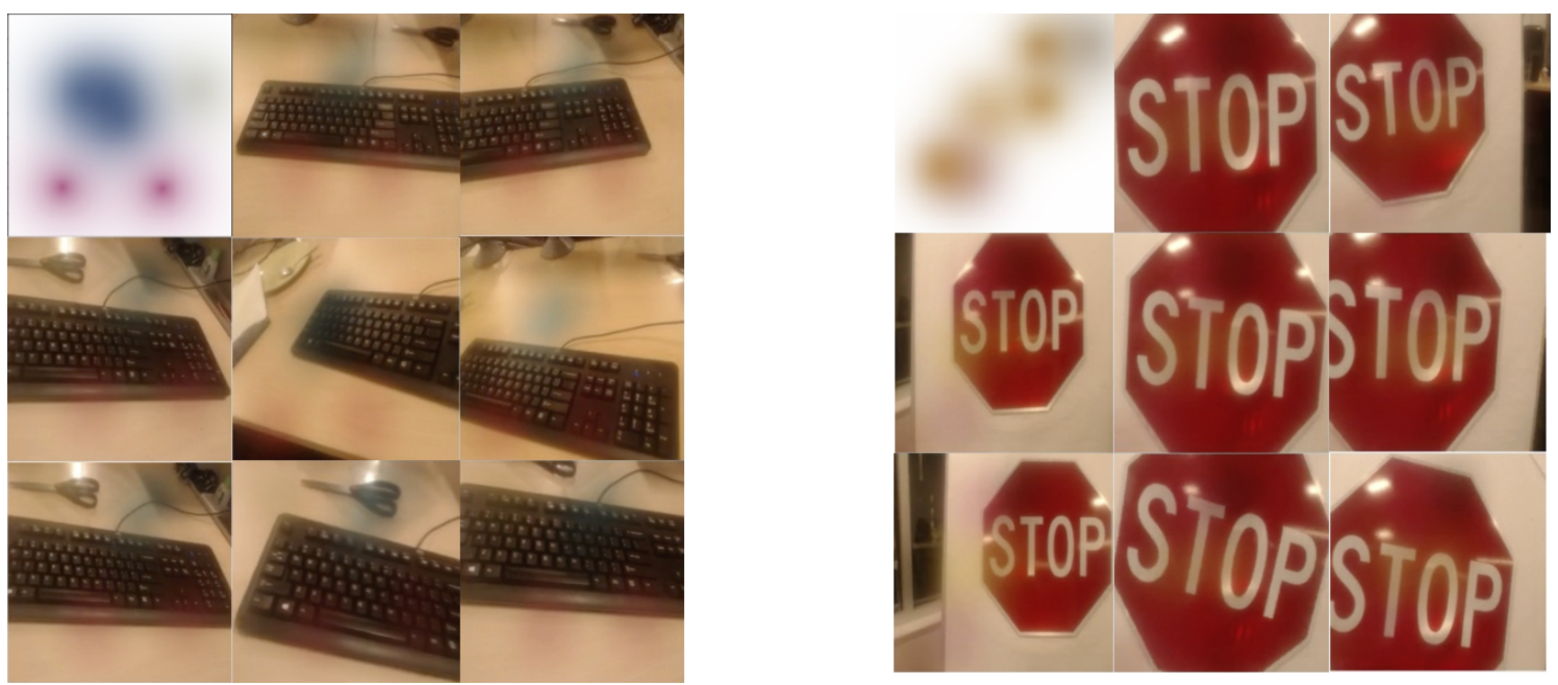
\includegraphics[width=12.0cm]{figures/adversarial-camera-example.pdf}
\end{center}
\caption{
作成した摂動とそれを印刷してカメラに貼って撮影した画像の例.
左側は {\it computer keyboard} クラスを {\it mouse} クラスに誤認識させていて, 右側は {\it street sign} クラスを {\it guitar pick} クラスに誤認識させている.
モデルは ILSVRC2012 pre-trained の ResNet-50 を用いている.
図は \cite{li2019adversarial} より引用.
}
\label{fig:adversarial-camera-example}
\end{figure}
%

作成した摂動の性能を定量的に測るため, 動画を 1,000 フレーム撮影してそれぞれを ILSVRC2012 pre-trained の ResNet-50 で予測した結果が図 \ref{fig:adversarial-camera-fool-ratio} である.
誤認識させることができたフレーム数は半分程度ではあるが, 確かに作成した摂動が有効に機能していることが示されている.
%
\begin{figure}[htbp]
\begin{center}
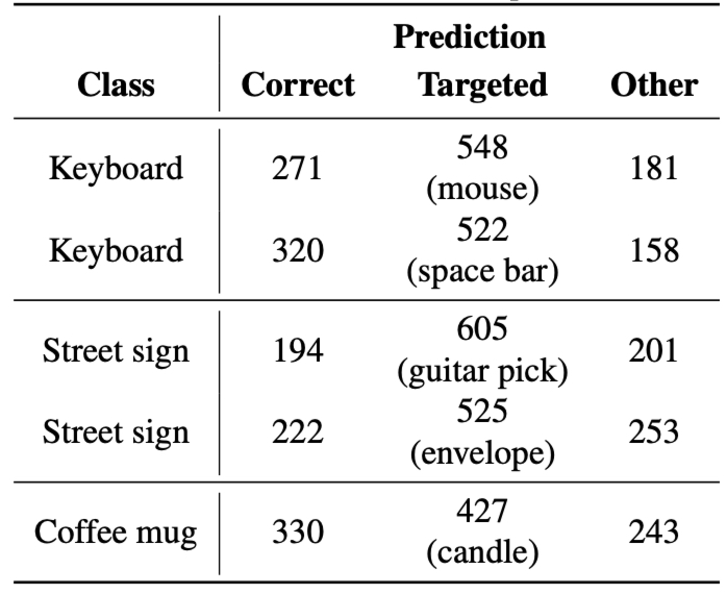
\includegraphics[width=6.0cm]{figures/adversarial-camera-fool-ratio.pdf}
\end{center}
\caption{
作成した摂動とそれを印刷してカメラに貼って動画を 1,000 フレーム撮影し, ILSVRC2012 pre-trained の ResNet-50 で予測させた結果.
図は \cite{li2019adversarial} より引用.
}
\label{fig:adversarial-camera-fool-ratio}
\end{figure}
%

この手法は, 対象物に摂動を加えるのではなくカメラのレンズにシールを貼るだけという点が新しい.
攻撃性能という意味では非常に高いものではないが, それでも数々のヒューリスティックも駆使しながら目的を実現している.
physical な攻撃に新たな展開をもたらした手法でもあり, 今後の更なる発展が期待される.



\subsection{Adversarial Examples for Semantic Segmentation and Object Detection}
\label{subsec:adversarial-examples}
%
\begin{table}[htbp]
\begin{center}
\begin{tabular}{|c|c|}
\hline
分類の観点 & この手法が該当するもの \\
\hline
Digital $\lor$ Physical & Digital \\
Classifier $\lor$ Detector & Detector \\
摂動作成時に使用するデータ & 攻撃対象データ \\
摂動の加え方 & 画像全体 \\
知覚しづらさの定義 & $l_2$ \\
White box $\lor$ Black box & White box \\
\hline
\multicolumn{2}{|c|}{公式実装: \href{https://github.com/cihangxie/DAG}{https://github.com/cihangxie/DAG}} \\
\hline
\end{tabular}
\label{tb:adversarial-example-summary}
\end{center}
\end{table}
%

これは \cite{xie2017adversarial} によって提案された手法であり, adversarial examples を object detection や semantic segmentation に拡張した.
基本的な戦略は classification で実施していた正しいラベルの logit の成分を小さくして間違えさせたいラベルの logit を大きくするという手法を, bbox やピクセルレベルで適用するものとなる.
bbox は入力データによって動的に変わるものなのでその影響を抑えるため NMS の閾値を高くしている.

この手法は detector に適用可能な攻撃手法であることが特徴で, それ以外の観点は典型的な classifier に対する digital attack と同様である.

detector の classifier との大きな違いは, 一つの入力データ $x$ に対して複数個の予測対象が存在するということであり, それを $\mathcal{T} = \{t_1, t_2, \dots, t_N\}$ と書く.
各対象 $t_n$ には正解ラベル $y_n \in \{1, 2, \dots, C\}$ が付与されている.
この各対象は object detection であれば bbox で, segmentation であればピクセルとなる.

それぞれの対象に対して logit の値を使って摂動を作成してそれを足しあわせていくというのが基本路線となるが, object detection の場合は入力データの変更によって検出される bbox の数が変わり得るため, 摂動を加えることで異なる bbox が検出されて変更したい予測ラベルに対する logit への効果が不十分となる可能性がある.
それを解決する一つの方法は, まずは多めに bbox を許しておいて, 摂動を加えても望み通りの振る舞いをする bbox のみを選択的に使っていく, というものである.
この論文では, NMS で用いる IoU の閾値を 0.70 から 0.90 に上げることで許容する bbox を増やし, さらに教師データの情報を用いて ground-truth との IoU が 0.1 以上で, かつその bbox の予測ラベルが $y_{\text{true}}$ である確率が 0.1 以上の bbox のみを残してそれ以外は除外する.
これにより, 攻撃対象は普通の object detection の場合よりも多くなり, 摂動を加えてそのうちのいくつかが (bbox として検出されなくなるなど) 期待に沿わない動きをしたとしても, 期待通りの動きをする bbox 数多く存在することで, 全体としては狙い通りの adversarial examples が作成できる.

予測対象 $\mathcal{T}$ が定められれば, アルゴリズム \ref{alg:adversarial-examples-alg} に従い摂動を作成することができる.
このアルゴリズムは論文では Dense Adversary Generation アルゴリズムと名付けられている.
規定回数に達するまで, 全ての予測対象が狙ったラベルに誤認識するまで loss function の微分に基づいて摂動を作成して足していく.
攻撃対象ラベルの集合は, それぞれの予測対象の正解ラベル以外のラベルからランダムに選ぶ.
途中の $\omega$ の規格化における factor $\gamma$ はハイパーパラメタであり論文では $0.5$ を使っている.
%
\begin{algorithm}
\caption{Dense Adversary Generation のアルゴリズム}
\label{alg:adversarial-examples-alg}
\begin{algorithmic}[1]
    \State Input: 入力データ $x$, モデル $f_{\text{label}}$, 予測対象 $\mathcal{T} = \{t_1, t_2, \dots, t_N\}$, 正解ラベルの集合 $\{y_1, y_2, \dots , y_N\}$, 攻撃対象ラベルの集合 $\{y_{\text{atk-tgt}, 1}, y_{\text{atk-tgt}, 2}, \dots , y_{\text{atk-tgt}, N}\}$, 最大反復回数 $K$.
    \State Output: 摂動 $\omega$.
    \State 初期化: $x_{\text{adv}}^{(0)} \leftarrow x, k \leftarrow 0, \mathcal{T}^{(0)} \leftarrow \mathcal{T}$.
    \While {$k < K$ and $\mathcal{T}^{(k)} \neq \emptyset$}
    \State $\mathcal{T}^{(k)} = \{ t_n | \argmax_{c} \left[ f_{\text{label}, c} (x_{\text{adv}}^{(k)}, t_n) \right] = y_n \}$.
    \State $\omega^{(k)} \leftarrow \sum_{t_n \in \mathcal{T}^{(k)}} \left[ \nabla_{x_{\text{adv}}^{(k)}} f_{y_{\text{label}, \text{atk-tgt}, n}} (x_{\text{adv}}^{(k)}, t_n) - \nabla_{x_{\text{adv}}^{(k)}} f_{\text{label}, y_{n}} (x_{\text{adv}}^{(k)}, t_n) \right]$.
    \State $\omega^{(k)} \leftarrow \frac{\gamma}{\| \omega^{(k)} \|_\infty} \omega^{(k)}$.
    \State $\omega \leftarrow \omega + \omega^{(k)}$.
    \State $x_{\text{adv}}^{(k + 1)} \leftarrow x_{\text{adv}}^{(k)} + \omega^{(k)}$.
    \State $k \leftarrow k + 1$.
    \EndWhile
\end{algorithmic} 
\end{algorithm} 
%

アルゴリズム \ref{alg:adversarial-examples-alg} では摂動の大きさの上限を定めるような機構は導入されていないため, 論文では以下の量を定義して知覚しづらさを定義し, これが小さいほど攻撃としてはうまくいっているものだと解釈している.
%
\begin{eqnarray}
p = \left( \frac{1}{\text{\# of pixels}} \| \omega \|_2 \right)^{1/2}.
\label{eq:adversarial-examples-imperceptibility}
\end{eqnarray}
%

実験は PascalVOC2007 データを用いて, object detection では Faster-RCNN, segmentation では FCN をいくつかの backbone モデルで構築して結果を調べている.
backbone モデルとしては AlexNet, ZF \cite{zeiler2014visualizing}, VGG, ResNet を採用している.
object detection と segmentation に対する adversarial examples の例が図 \ref{fig:adversarial-examples-example} である.
同一の摂動によってどちらも誤認識していて, 提案手法の性質により, segmentation はラベルの位置自体は元のものから大きくは変わっていないが, object detection は bbox の位置や大きさが大きく変わっている.
%
\begin{figure}[htbp]
\begin{center}
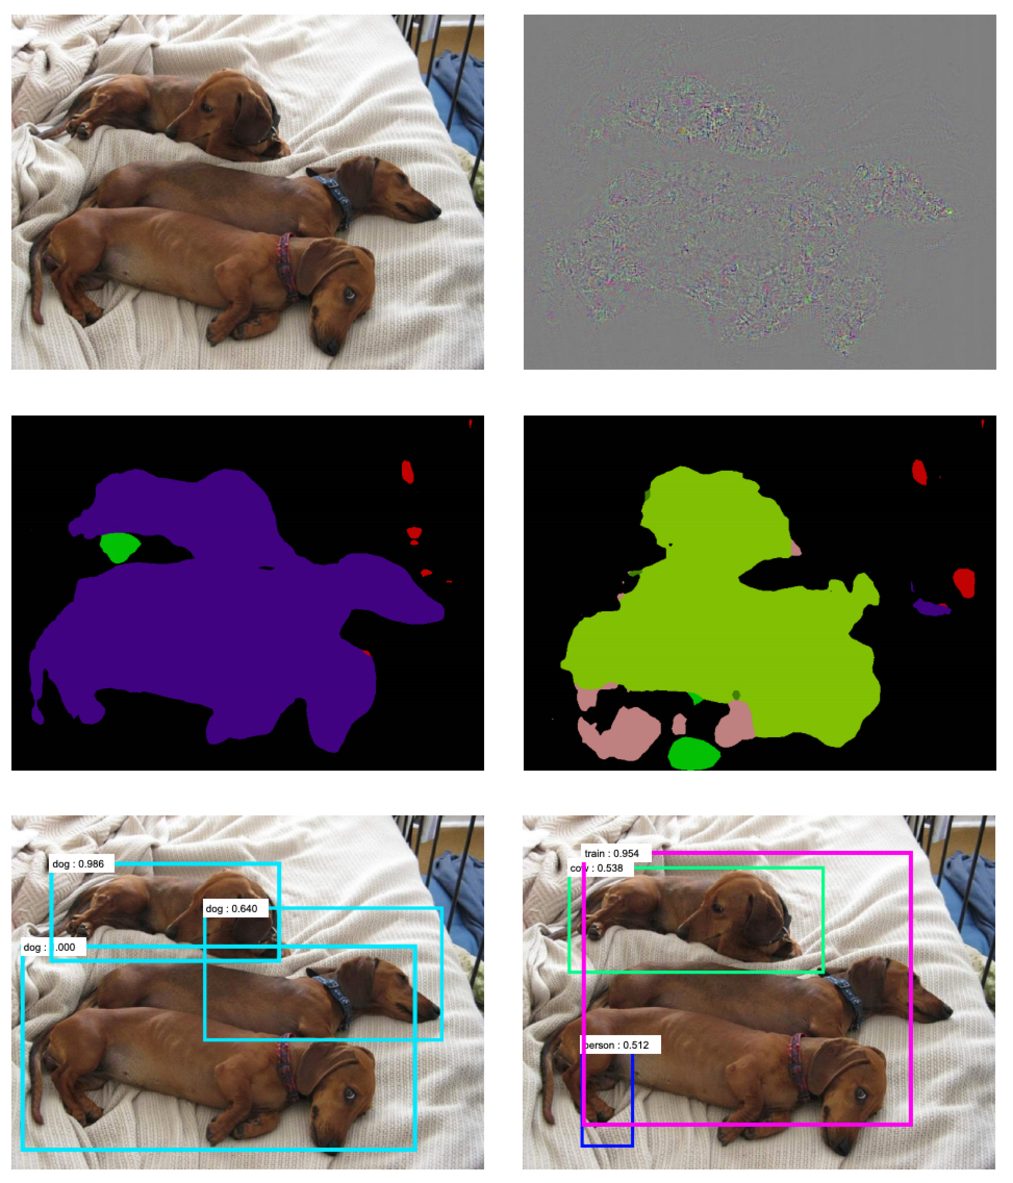
\includegraphics[width=10.0cm]{figures/adversarial-examples-example.pdf}
\end{center}
\caption{
object detection と segmentation に対する摂動とその効果の例.
上の行は左列が入力画像で右列が摂動, 真ん中の行は左列が入力画像に対する segmentation の結果で右列が adversarial examples に対する segmentation の結果, 下の行は object detection の結果である.
摂動に関しては画像として見やすいように大きさが 10 倍されている.
segmentation において, 紫色が {\it dog} のラベルで黄緑色が {\it train} ラベルである.
図は \cite{xie2017adversarial} より引用.
}
\label{fig:adversarial-examples-example}
\end{figure}
%

定量的な結果は object detection が図 \ref{fig:adversarial-examples-result-object-detection} で segmentation が図 \ref{fig:adversarial-examples-result-segmentation} である.
摂動の作成は, object detection では ZF と VGG, segmentation では AlexNet と VGG で実施しており, ResNet は予測モデルとしてのみ使用している.
どちらの結果も white box attack では大きく性能が低下しており, 提案手法の攻撃が確かに機能していることが分かる.
モデルの構造が似ている場合は transferability も高いが, 一方で ResNet への影響は少なく, 攻撃性能はかなりモデル構造に依存している.
摂動を足し合わせることでそれぞれのモデルの性能が低下しているため, 摂動にある種の線形性があることも伺える.
また, permutate した結果はほとんど摂動なしの結果と変わらないことから, 摂動は単にその大きさが重要なのではなく, 意味のある位置に配置して摂動が増幅されるようになっている必要があることも示されている.
%
\begin{figure}[htbp]
\begin{center}
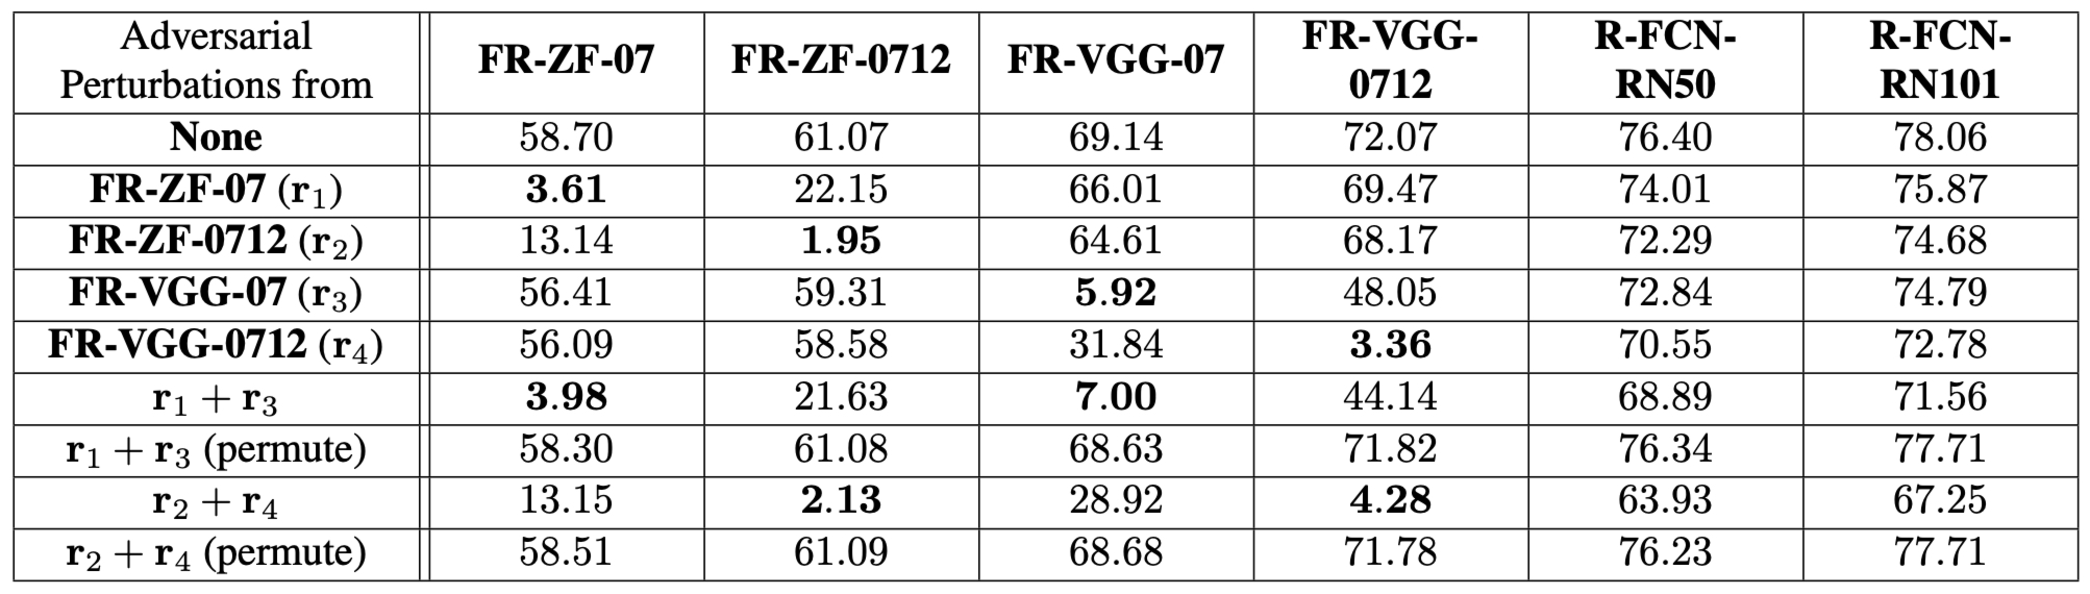
\includegraphics[width=14.0cm]{figures/adversarial-examples-result-object-detection.pdf}
\end{center}
\caption{
PascalVOC2007 の 4,952 枚のテストデータに対する結果.
表の値は mAP で $r$ は摂動 $\omega$ と対応している.
$r_1 + r_3$ (permute) は, それぞれのモデルで得られた摂動を足した後に, 行や列をランダムに入れ替えて作成した摂動である.
図は \cite{xie2017adversarial} より引用.
}
\label{fig:adversarial-examples-result-object-detection}
\end{figure}
%
%
\begin{figure}[htbp]
\begin{center}
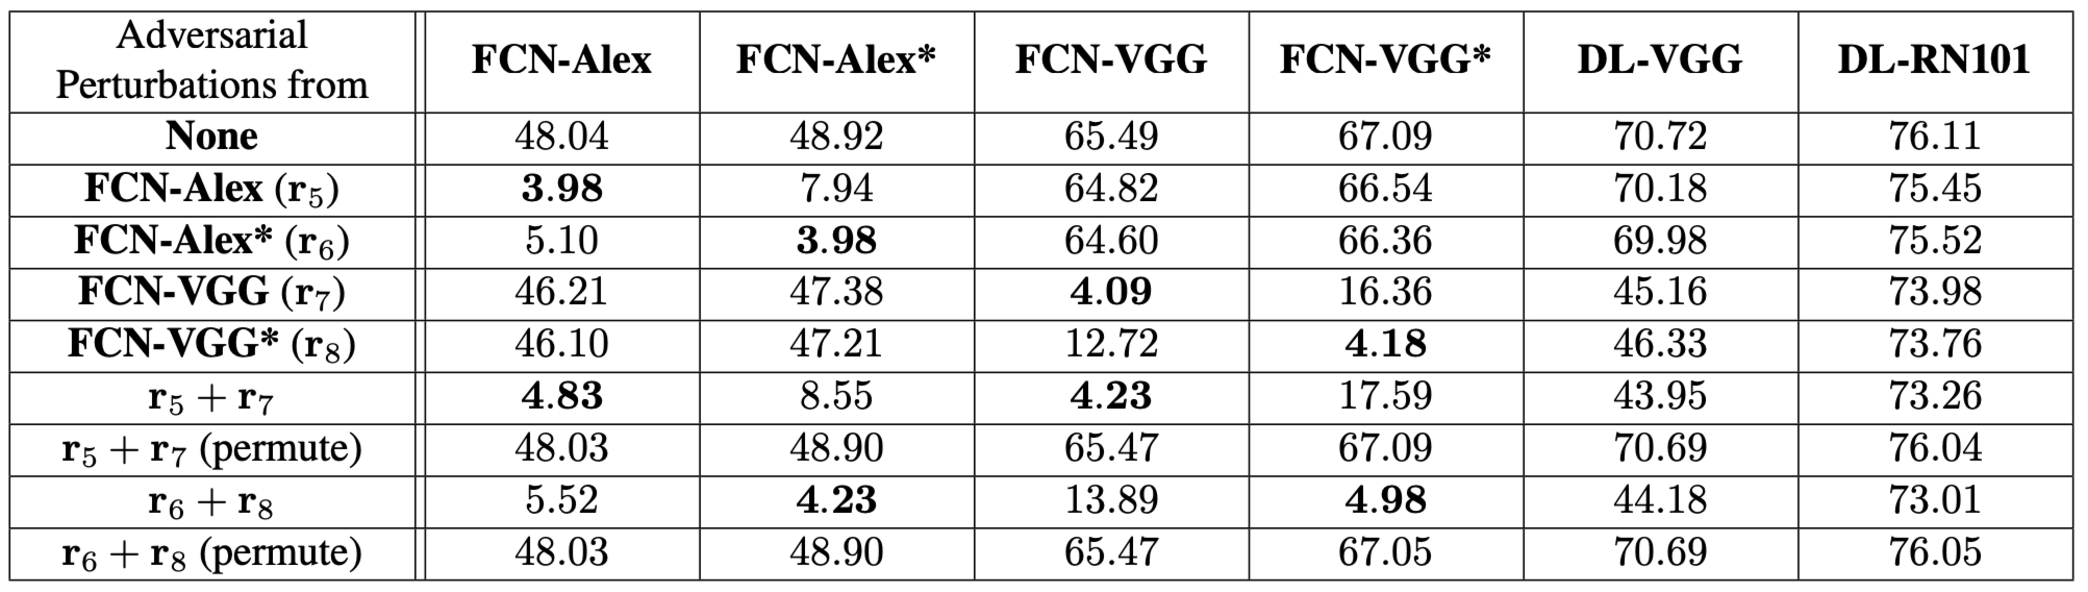
\includegraphics[width=14.0cm]{figures/adversarial-examples-result-segmentation.pdf}
\end{center}
\caption{
PascalVOC2007 の 736 枚の検証データに対する結果.
表の値は mIoU で $r$ は摂動 $\omega$ と対応している.
$r_1 + r_3$ (permute) は, それぞれのモデルで得られた摂動を足した後に, 行や列をランダムに入れ替えて作成した摂動である.
図は \cite{xie2017adversarial} より引用.
}
\label{fig:adversarial-examples-result-segmentation}
\end{figure}
%

認識のしづらさとして定義した式 \ref{eq:adversarial-examples-imperceptibility} を用いると, どの摂動に対しても $1.5 \sim 3.0 \times 10^{-3}$ という値になっていてそこまで大きな違いはない.
図 \ref{fig:adversarial-examples-example} で見たように, classification と同様に人間にとっては違いは認識しづらいレベルになっている.

この手法は, classification に対する adversarial examples を object detection は segmentation に拡張したという点で興味深い.
object detection に対する adversarial examples は自動運転などの応用を考えると高い重要性を持っており, このような論文をきっかけに攻撃やその防御方法などが広く研究されるようになってきている.
object detection に対する adversarial examples が出始めたころは \cite{lu2017no} で自動運転においては撮影の距離や角度が変わるので誤認識はされないという議論もなされたりもしたが, その後すぐに物理的環境の変化があっても高い割合で誤認識させる攻撃手法も提案され, 以降は object detection の研究も盛んに進められていて, この分野の発展の早さが感じられる.



\subsection{DARTS: Deceiving Autonomous Cars with Toxic Signs}
\label{subsec:darts}
%
\begin{table}[htbp]
\begin{center}
\begin{tabular}{|c|c|}
\hline
分類の観点 & この手法が該当するもの \\
\hline
Digital $\lor$ Physical & Physical \\
Classifier $\lor$ Detector & Detector-Classifier パイプライン \\
摂動作成時に使用するデータ & 攻撃対象データ \\
摂動の加え方 & 対象物のみ \\
知覚しづらさの定義 & $l_2$ \\
White box $\lor$ Black box & White box \\
\hline
\multicolumn{2}{|c|}{公式実装: \href{https://github.com/chawins/DART}{https://github.com/chawins/DART}} \\
\hline
\end{tabular}
\label{tb:darts-summary}
\end{center}
\end{table}
%

これは \cite{sitawarin2018darts} によって提案された手法であり, 動画から Canny 法によるエッジ検出と Hough 変換を使って標識部分を切り出し, それを classifier で分類するというパイプラインに対して異なる標識と誤認識させる.
また, 摂動を加える以外にも, 見る角度によって異なる標識になるようなレンチキュラー印刷による攻撃手法も提案している.

この手法は detector を攻撃対象とした physical な攻撃ではあるが, 想定している予測モデルは detector ではなく, 図 \ref{fig:darts-pipeline} のように, DNN 以前の手法での detector と DNN による classifier をつなぎ合わせたパイプラインを攻撃対象としている点が特徴的である.
%
\begin{figure}[htbp]
\begin{center}
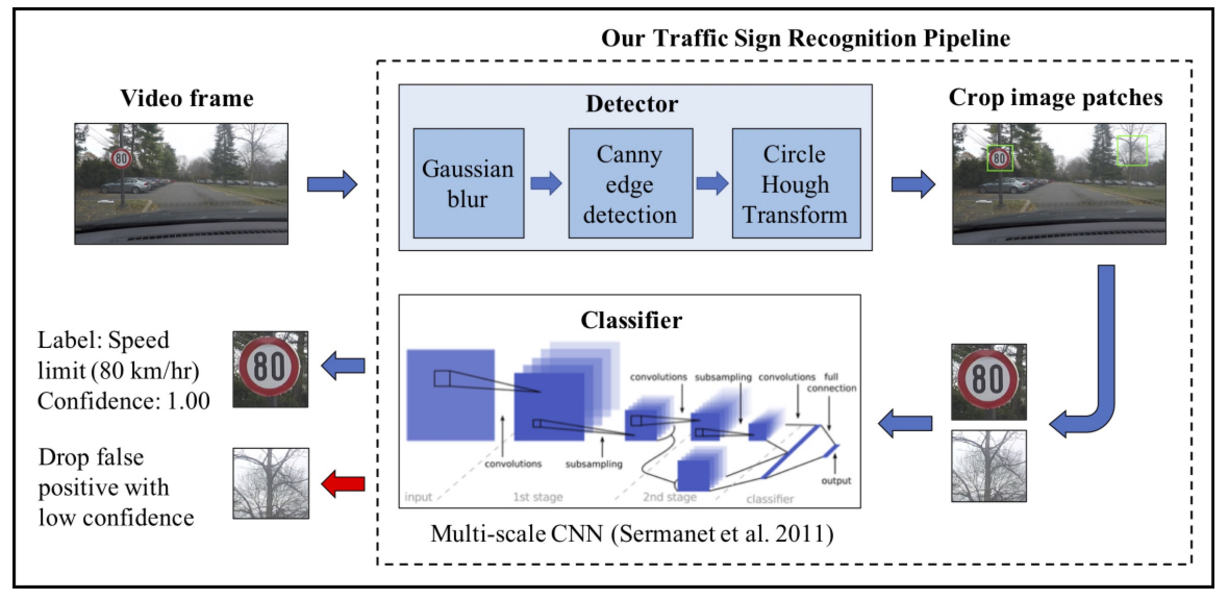
\includegraphics[width=14.0cm]{figures/darts-pipeline.pdf}
\end{center}
\caption{
攻撃対象となる detector-classifier pipeline の概略図.
動画の書くフレームにおいて, まず Canny 法でエッジを検出してからハフ変換を用いて標識の円部分を検出し, 該当部分を cropping して classifier で予測するという流れになっている.
図は \cite{sitawarin2018darts} より引用.
}
\label{fig:darts-pipeline}
\end{figure}
%

全体としては自動運転システムを対象にした攻撃になっているが, adversarial examples で攻撃するのは標識部分を crop した画像を入力とする classifier である.
そのため, adversarial examples の作り方自体は classifier を対象とした場合と違いはない.
この論文では標識のみをターゲットにしているため, 円形の対象物に特化した手法で, Canny 法でエッジを検出することで円部分のみを切り出す mask を作る.
mask を使うというのは \ref{subsec:robust-physical} 節で紹介した手法と同様のアプローチで, 標識部分のみに摂動を加えるためにこの mask を用いている.
摂動を作成するために解く最適化問題としては以下を設定している.
%
\begin{eqnarray}
\min_{\omega} \left[ \frac{c}{B} \sum_b^B F(\tau_b (x + M \cdot \omega)) + \max (\| \omega \|_p, L) \right].
\label{eq:darts-optimization}
\end{eqnarray}
%
ここで, $B$ はバッチサイズ, $F(x) = \max ( \max_{j \neq t} \{f_{\text{logit}, j} (x)\} - f_{\text{logit}, t} (x), - K)$ は loigt loss, $M$ は標識部分のみを残す mask, $\tau_b$ は回転などの幾何学変換, である.
$c, K, L$ はうまく解が求まるようにヒューリスティックに調整するパラメタである.
ノルムは任意のものを使えるが, 論文では $p = 1$ を採用している.
この最適化問題を Adam \cite{kingma2014adam} を用いて解くことで摂動を作成する.
adversarial examples 作成の全体図は図 \ref{fig:darts-attack-pipeline} である.
%
\begin{figure}[htbp]
\begin{center}
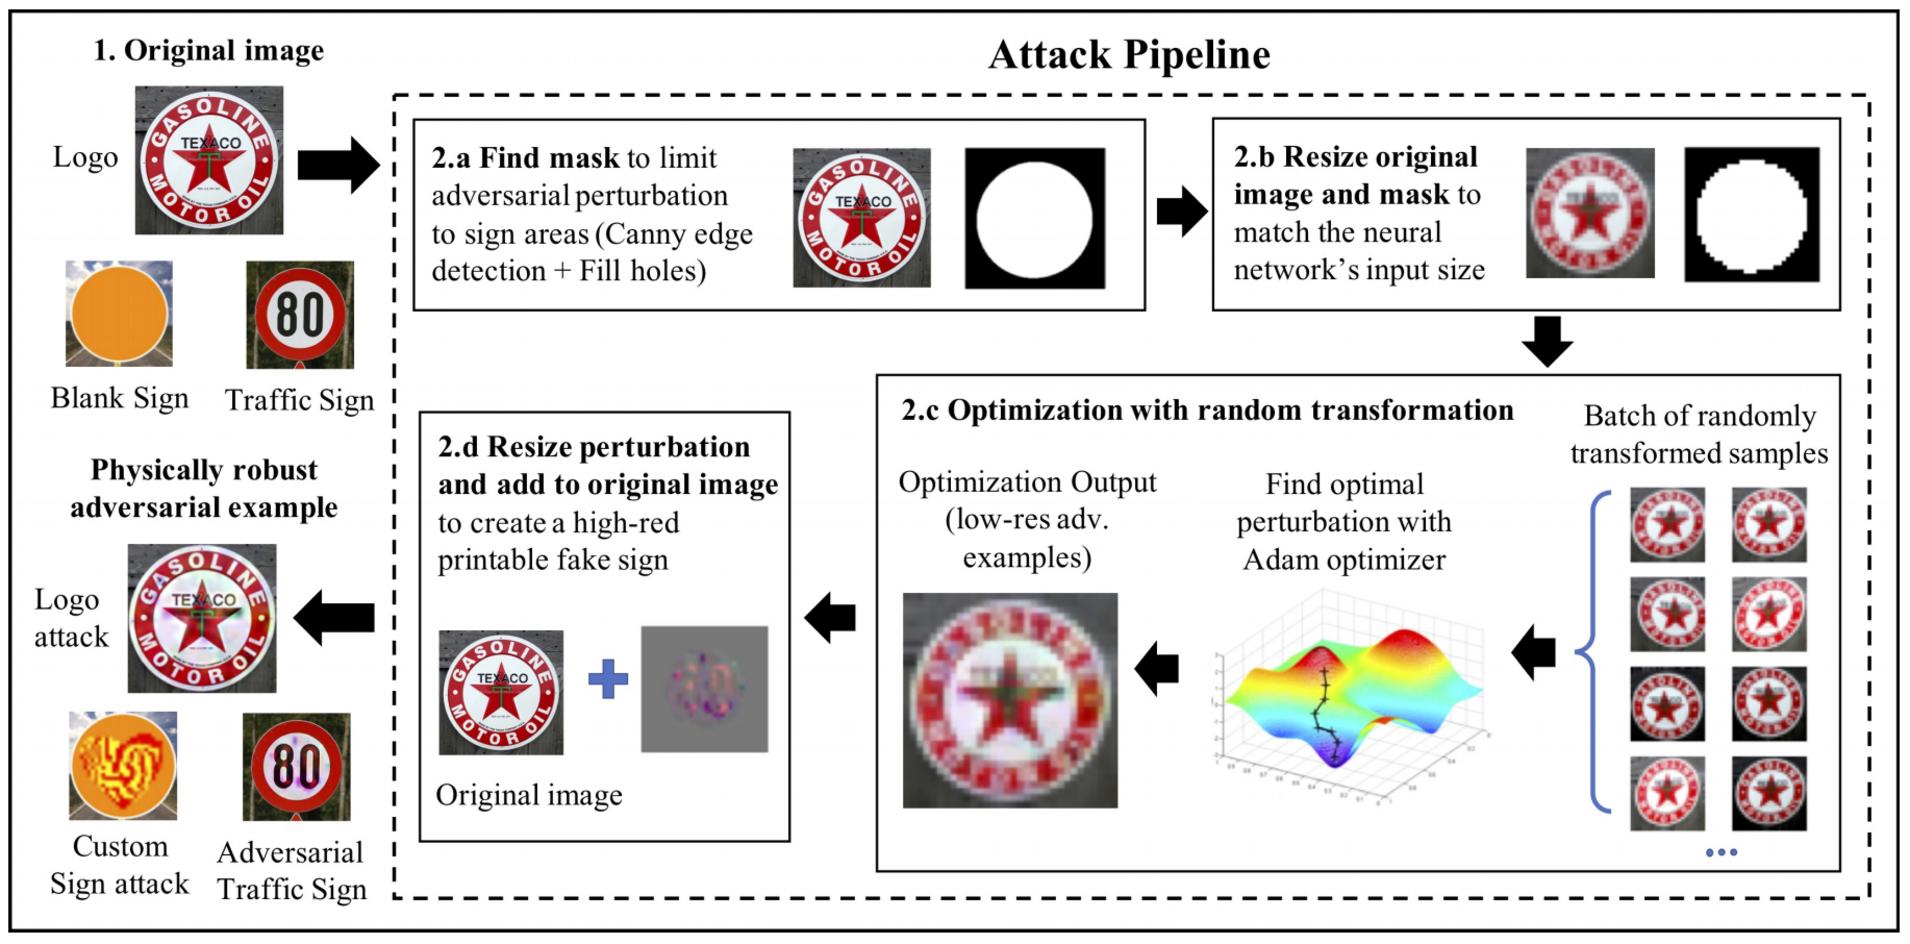
\includegraphics[width=14.0cm]{figures/darts-attack-pipeline.pdf}
\end{center}
\caption{
adversarial examples 作成の手順.
標識部分を切り出す mask を作成し, 様々な幾何学変換を加えたサンプルを誤認識させる摂動を式 \ref{eq:darts-optimization} を Adam で解くことで作成する.
図は \cite{sitawarin2018darts} より引用.
}
\label{fig:darts-attack-pipeline}
\end{figure}
%

摂動が作成できれば, それは円形で標識の形にマッチしているので, 紙などに印刷して標識の上から貼り付けることで自動運転システムを攻撃することができる.
この論文では, 標識以外にも円形のロゴに対する摂動や, 無地の円形図形に特定の模様や文字の摂動 (そのような mask を準備すれば実現できる) を作成している.
その結果が図 \ref{fig:darts-example} であり, 作成した摂動が classifier を誤認識させていることが分かる.
%
\begin{figure}[htbp]
\begin{center}
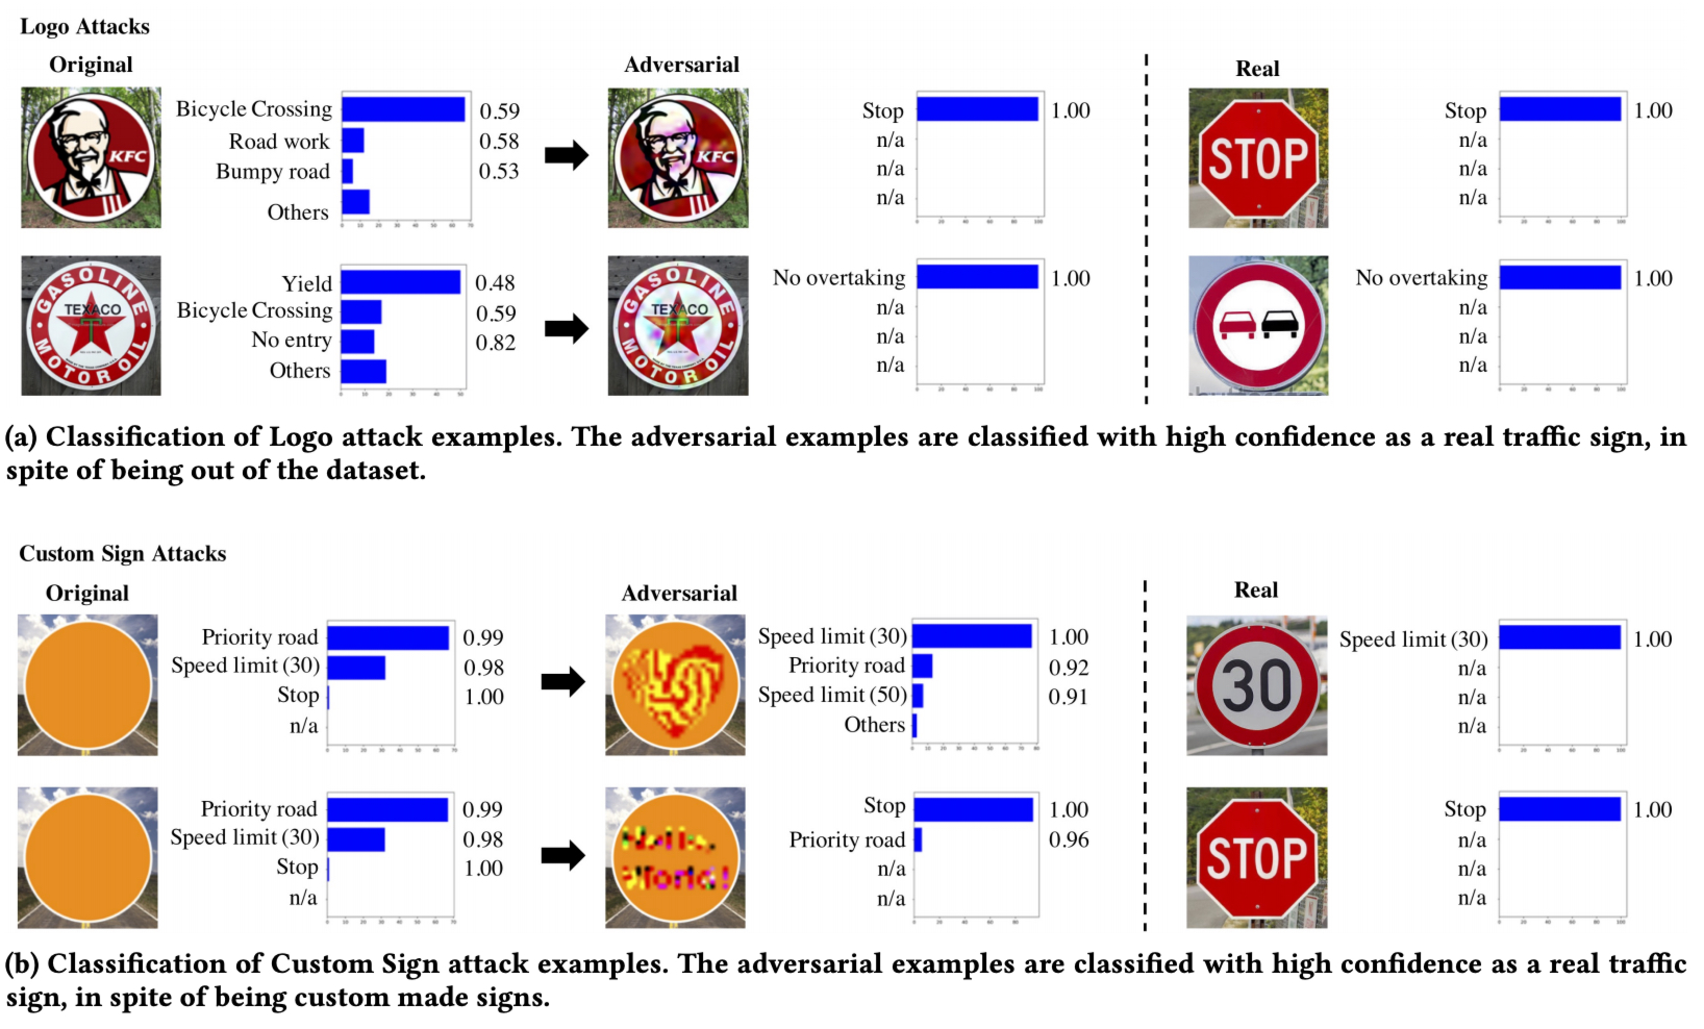
\includegraphics[width=14.0cm]{figures/darts-example.pdf}
\end{center}
\caption{
作成した摂動の例とそれに対する classifier の予測結果.
予測結果のラベルと数値は 100 個の異なる幾何学変換を加えて予測した際の top-1 の結果をカウントしたものと confidence の平均を表す.
Original は摂動を加える前の画像で, classifier は標識のラベルを予測するようになっているのでうまく予測できていないが, 摂動を加えたものは明白に何かの標識に誤認識している.
Real は実際の標識画像に対して classifier が適切に予測していることを示している.
図は \cite{sitawarin2018darts} より引用.
}
\label{fig:darts-example}
\end{figure}
%

実験は様々なものを実施しているが, 特に興味深い drive-by test のみに言及する.
作成した摂動は前述のように印刷して physical attack として利用できるため, 実験用に adversarial examples となる標識を準備し, 車に GoPro HERO5 を設置して撮影した動画で検証をしている.
モデルは multi-scale CNN \cite{sermanet2011traffic} を用いている.
結果は図 \ref{fig:darts-result-table} の通りで, 提案手法の攻撃が physical attack として有効に機能していることが示されている.
black box attack の攻撃成功率がやたらと高く出ているが, ここでの black box attack は攻撃者はモデルとしては同じものを用いるが学習自体は別個に実施して, 摂動作成時には実際の予測モデルではなく自分が学習したモデルを使う, という設定になっているためである.
これは実質 white box と言ってよいだろう.
%
\begin{figure}[htbp]
\begin{center}
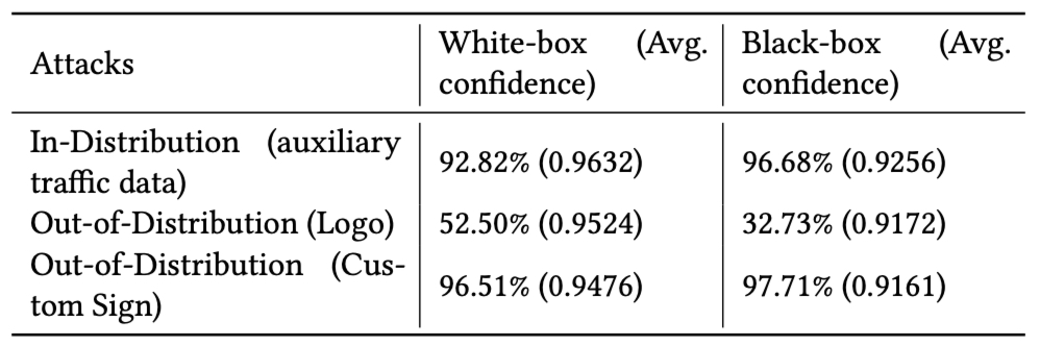
\includegraphics[width=12.0cm]{figures/darts-result-table.pdf}
\end{center}
\caption{
adversarial examples となる標識を設置して, 実際に車から撮影した動画で誤認識率 (1 - 正答率) を測定した結果.
auxiliary traffic data は標識の画像データを基にして摂動を作成した場合となる.
図は \cite{sitawarin2018darts} より引用.
}
\label{fig:darts-result-table}
\end{figure}
%

また, この論文ではレンチキュラー印刷による攻撃手法も提案している.
レンチキュラー印刷とは凸型の表面を利用した印刷方法で, 見る角度によって異なる対象物が見えるものである.
車載カメラが運転者の目線よりも低い位置に付けられるということを想定し, 下から撮影すると別の標識に認識されるような印刷物を作成し, 期待通りに攻撃が成功したことも報告している.
これはこれで興味深いが, DNN に対する adversarial examples とは独立な手法であるため, 本書ではこれ以上は立ち入らない.

この手法は単一の DNN detector ではなく, DNN 以前の手法による detector と DNN classifier パイプラインに対する攻撃手法を提案したという点が興味深い.
近年の DNN の性能を考えればこのようなパイプラインを実際に使用する可能性はあまり高くはないと思われるが, physical attack でありながらも標識の classifier をターゲットにすることで誤認識率の高い adversarial examples を作成することに成功している.
自動運転に限らず, いくつかのモデルを組み合わせたパイプラインに対して, 攻撃対象を絞ることで攻撃効率を高めるというのは攻撃側にとっては有効な選択肢になるだろう.



\subsection{ShapeShifter: Robust Physical Adversarial Attack on Faster R-CNN Object Detector}
\label{subsec:shapeshifter}
%
\begin{table}[htbp]
\begin{center}
\begin{tabular}{|c|c|}
\hline
分類の観点 & この手法が該当するもの \\
\hline
Digital $\lor$ Physical & Physical \\
Classifier $\lor$ Detector & Detector \\
摂動作成時に使用するデータ & 攻撃対象データ \\
摂動の加え方 & 対象物のみ \\
知覚しづらさの定義 & $l_2$ \\
White box $\lor$ Black box & White box \\
\hline
\multicolumn{2}{|c|}{公式実装: \href{https://github.com/shangtse/robust-physical-attack}{https://github.com/shangtse/robust-physical-attack}} \\
\hline
\end{tabular}
\label{tb:shapeshifter-summary}
\end{center}
\end{table}
%

これは \cite{chen2018shapeshifter} によって提案された手法であり, Faster-RCNN に対して候補領域の予測に対する loss が高まるように摂動を作り攻撃をする\footnote{
技術的な内容とはあまり関係がないが, shapeshifter とは様々な姿に変身することができる妖怪のことである.
}.

この手法は detector をターゲットにして, physical attack でも誤認識率が高くなるような摂動を作成したという点が特徴的である.
それを実現するために, mask と classifier と比べて強めの摂動を用いている.

まず, classifier に対する攻撃を構成する.
この手法ではピクセル値として $[-1, 1]$ の範囲を取るように画像を正規化する.
作成する adversarial examples がこの範囲に収まるようにするためには $\tanh$ を利用する.
CW の方法に従い, 以下の最適化問題を解くことで摂動を作成する.
%
\begin{eqnarray}
\argmin_{x_{\text{adv}}} \left[ J (f, \tanh (x_{\text{adv}}), y_{\text{atk-tgt}}) + c \cdot \| \tanh (x_{\text{adv}}) - x \|_2 \right].
\label{eq:shapeshifter-classifier}
\end{eqnarray}
%
次にこれを physical attack に適したものにするために特定の対象物に限定することを考える.
これは \ref{subsec:darts} 節で紹介した手法と同様で重要な点は二つあり, 一つは mask を用いて対象物にのみ摂動を加えるようにすることで, もう一つは様々な幾何学変換を適用して異なる距離や角度から撮影しても摂動が有効になるようにすることである.
ここでは, ある特定の対象物部分のみの画像を $x_o$ として mask の処理を $M_{x^o} (x)$ とし,  幾何学変換を $t(x)$ とする.
これらを用いて式 \ref{eq:shapeshifter-classifier} を変更すると以下のように書ける.
%
\begin{eqnarray}
\argmin_{x_{\text{adv}}} \mathbb{E}_{x \sim p_x, t \sim p_t} \left[ J (f, t(M_{x^o} (\tanh (x_{\text{adv}}))), y_{\text{atk-tgt}}) + c \cdot \| \tanh (M_{x^o} (x_{\text{adv}})) - x \|_2 \right].
\label{eq:shapeshifter-classifier-object-oriented}
\end{eqnarray}
%
ただし, $x$ はある特定のクラスに属するもので何かしらの分布から生成されているものとし, $t$ も何かしらの変換の分布から生成されていると定式化している.

これを detector に拡張することを考える.
Faster-RCNN は RPN で検出した候補領域で予測をするモデルであるので, それを考慮して mask した上での候補領域 $r_1, \dots, r_m$ を対象にした loss に変更すればよい.
%
\begin{eqnarray}
\argmin_{x_{\text{adv}}} \mathbb{E}_{x \sim p_x, t \sim p_t} \left[ \frac{1}{m} \sum_{r_i \in RPN (t(M_{x^o} (\tanh (x_{\text{adv}}))))} J (f, r_i, y_{\text{atk-tgt}}) + c \cdot \| \tanh (M_{x^o} (x_{\text{adv}})) - x \|_2 \right].
\label{eq:shapeshifter-detector}
\end{eqnarray}
%
これは候補領域毎に loss を計算しているという違いはあるが, 本質的には classifier のものと同じである.
全ての候補領域が固定されていればこのままでよいが, NMS などの微分不可能な仕組みで候補領域が変更されるため, このままではこの最適化を解くのは難しい.
この論文では, まずは RPN だけを対象にして最適化を Adam などを使って近似的に解き, RPN が返す候補領域を固定してしまう.
予測ステージではこの予測領域は固定したまま予測モデル部分に対して改めて最適化を解くことで, adversarial examples を作成する.
論文ではこの近似で十分に良い adversarial examples が作成できると主張している.

adversarial examples 作成のためのデータは MSCOCO2017 データ \cite{lin2014microsoft} の {\it stop sign} クラスを用いる.
これは mask を作成するのが楽で, かつ印刷をして physical attack の実験をするのにも適している.

実際に physical attack をしてみた例が図 \ref{fig:shapeshifter-result-physical} である.
クラスが {\it sports ball} の場合は狙い通りに誤認識させることが難しいが, {\it person} もしくは utntargeted の場合は攻撃が成功しているのが見て取れる.
%
\begin{figure}[htbp]
\begin{center}
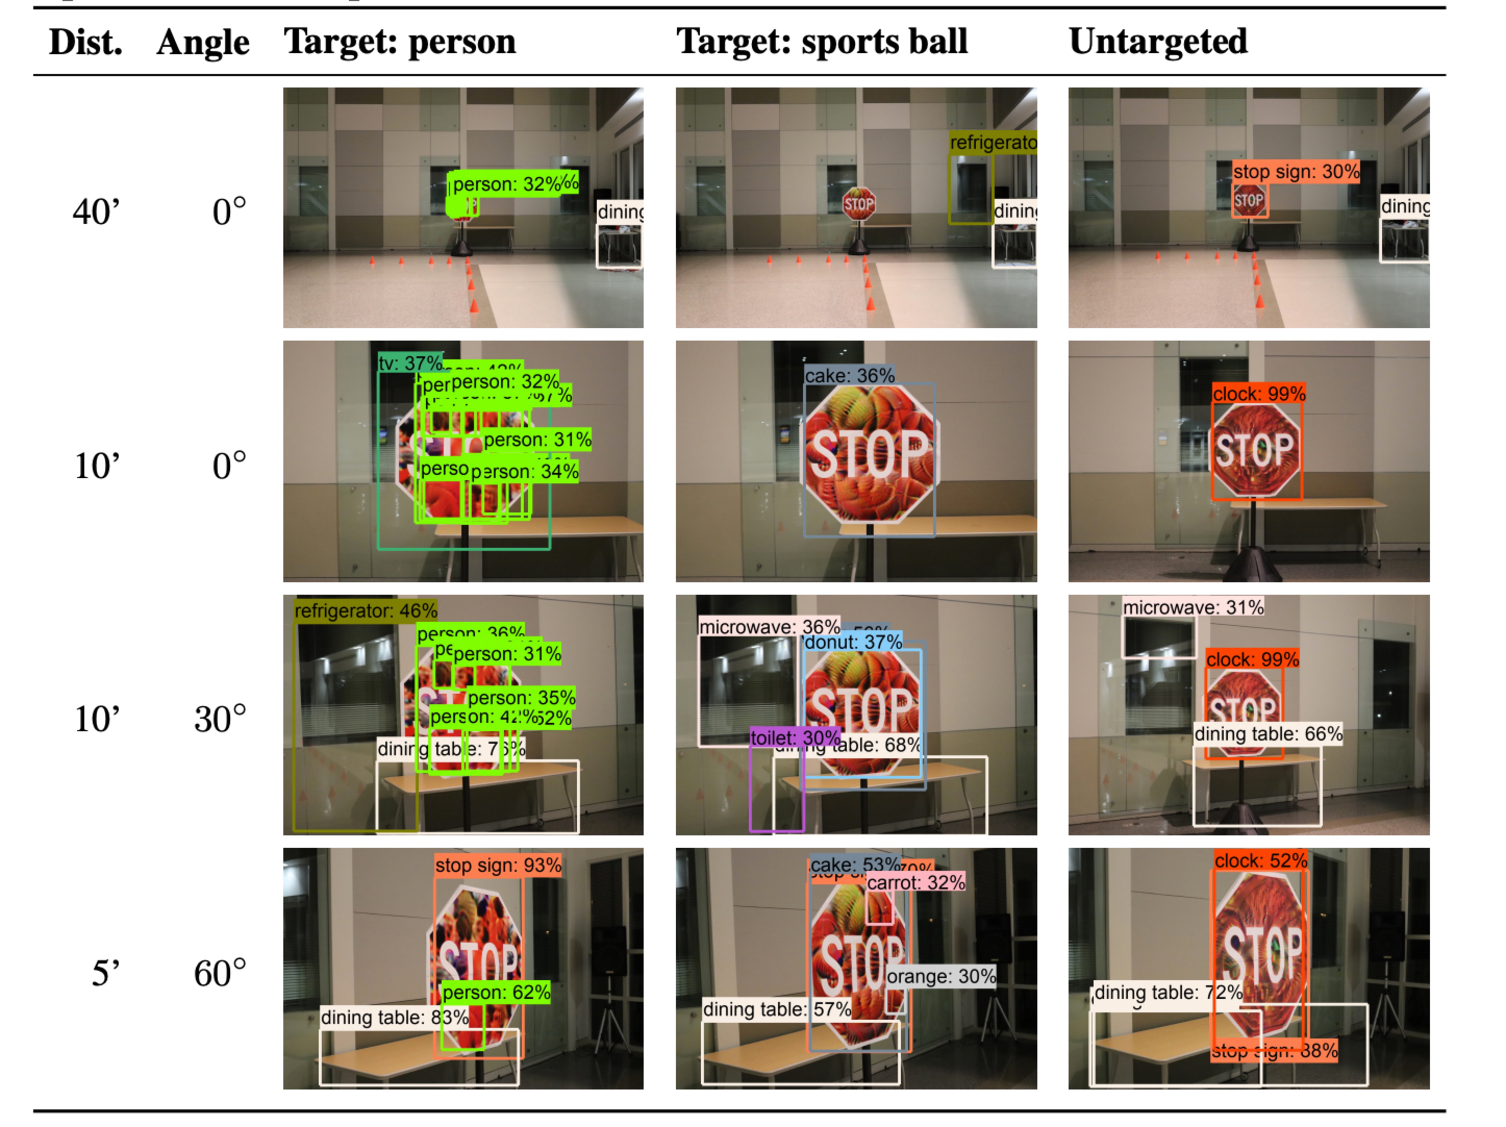
\includegraphics[width=14.0cm]{figures/shapeshifter-result-physical.pdf}
\end{center}
\caption{
physical attack の例.
MSCOCO2017 の {\it stop sign} クラスの画像で摂動を作成し, それをプリントしたものを様々な距離や角度から撮影して Faster-RCNN で予測している.
図は \cite{chen2018shapeshifter} より引用.
}
\label{fig:shapeshifter-result-physical}
\end{figure}
%

physical attack は性能の測定が難しく, 従来手法では雑に動画を撮って各フレームで調べるという程度でしか調べられていなかったが, この論文では静止画限定ではあるがもう少し定量的な評価指標を構築している.
図 \ref{fig:shapeshifter-measurement} のように距離と角度を指定して撮影し, それぞれの画像で正答率を調べることで physical attack の異なる環境での有効性を検証している.
%
\begin{figure}[htbp]
\begin{center}
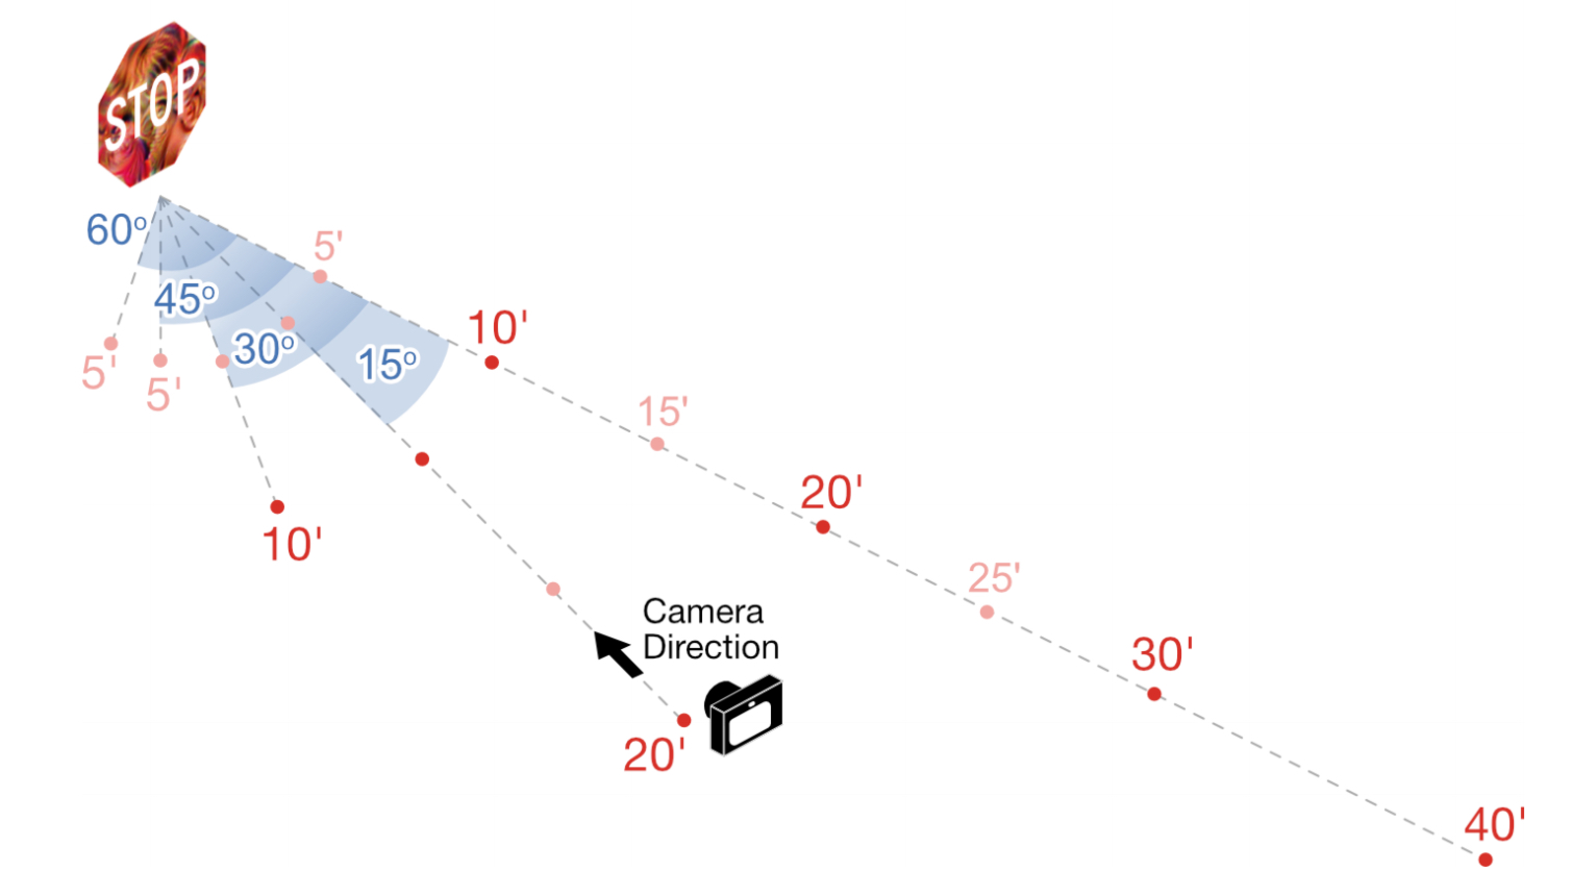
\includegraphics[width=12.0cm]{figures/shapeshifter-measurement.pdf}
\end{center}
\caption{
静止画の physical attack に対する測定方法.
角度は $\{0^{\circ}, 15^{\circ}, 30^{\circ}, 45^{\circ}, 60^{\circ}\}$ で, 距離は角度に応じて $5$ フィート (約 $1.5$ メートル) から $40$ フィート (約 $12$ メートル) である.
図は \cite{chen2018shapeshifter} より引用.
}
\label{fig:shapeshifter-measurement}
\end{figure}
%

静止画で定量的に測定した結果が図 \ref{fig:shapeshifter-result-table} である.
どのクラスに間違えさせるかで性能も変わってくるが, {\it person} ではほとんどの距離や角度で誤認識させることに成功している.
ただし, 角度がキツくなると誤認識させることは失敗している.
%
\begin{figure}[htbp]
\begin{center}
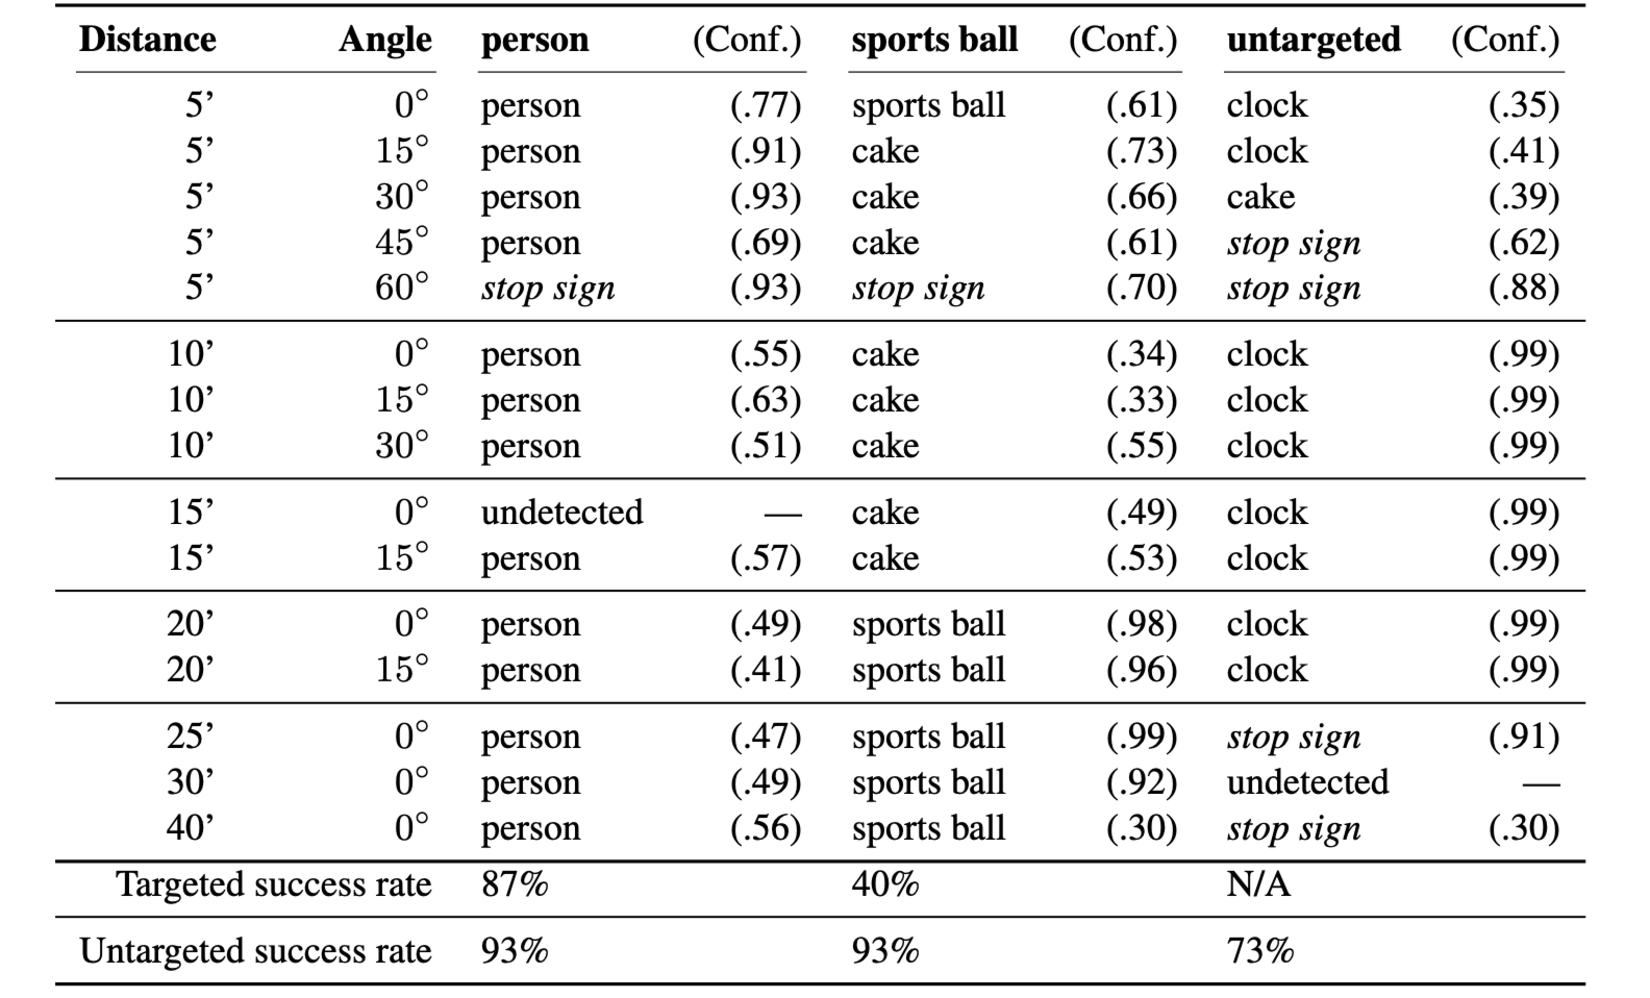
\includegraphics[width=14.0cm]{figures/shapeshifter-result-table.pdf}
\end{center}
\caption{
physical attack に対する静止画の定量的評価.
図 \ref{fig:shapeshifter-result-physical} で定義した距離と角度で画像を撮影し, Faster-RCNN の予測結果の confidence が最も高いものを記載している.
success rate は攻撃成功率 (1 - 正答率) を表す.
図は \cite{chen2018shapeshifter} より引用.
}
\label{fig:shapeshifter-result-table}
\end{figure}
%

動画での検証も実施しており, 車からスマートフォンで動画を撮影して各フレームで Faster R-CNN の予測を評価している.
{\it person} クラスに誤認識させる摂動の場合, 405 フレーム中, 1 フレームは {\it stop sign}, 190 フレームは {\it person}, 残りの 214 フレームは検出されず, という結果になっている.
{\it sports ball} クラスに誤認識させる摂動も同じような結果だが, untargeted の場合はほとんどが未検出という結果になっている.
untargeted の場合になぜ静止画での評価との乖離が大きいかというのは著者はよく分からない.

この手法は, Faster-RCNN を対象にした physical attack として高い攻撃成功率を達成した点が興味深い.
physical attack で高い攻撃成功率を達成するためには摂動はかなり強いものにする必要があるが, mask と合わせて性能の高い physical attack を実現した.
また, 静止画ではあるが physical attack の定量的評価を提示したというのも重要な点である.
全部で 15 枚の予測であるので数としては心許ないが, 再現性や比較のために共通の評価方法が確立されることが期待される.



\subsection{Daedalus: Breaking Non-Maximum Suppression in Object Detection via Adversarial Examples}
\label{subsec:daedalus}
%
\begin{table}[htbp]
\begin{center}
\begin{tabular}{|c|c|}
\hline
分類の観点 & この手法が該当するもの \\
\hline
Digital $\lor$ Physical & Digital \\
Classifier $\lor$ Detector & Detector \\
摂動作成時に使用するデータ & 攻撃対象データ \\
摂動の加え方 & 画像全体 \\
知覚しづらさの定義 & $l_0, l_2$ \\
White box $\lor$ Black box & White box \\
\hline
\multicolumn{2}{|c|}{公式実装: \href{https://github.com/NeuralSec/Daedalus-attack}{https://github.com/NeuralSec/Daedalus-attack}} \\
\hline
\end{tabular}
\label{tb:daedalus-summary}
\end{center}
\end{table}
%

これは \cite{wang2019daedalus} によって提案された手法であり, NMS に対して摂動で攻撃を加えることで大量の誤った bbox を認識させるという攻撃手法である\footnote{
技術的な内容とは関係ないが, daedauls は日本語ではダイダロスで, ギリシャ神話においてミノタウルスを封じ込めるために迷宮を作った.
}.

この手法は detector の予測を間違えさせるというアプローチではなく, 大量の bbox が発生するように誤認識させるという点が特徴的である.

定式化のためにいくつか記法を導入する.
detector を $F(x) = \{ B^x, B^y, B^w, B^h, B^o, P \}$ という関数とする.
ここで, $n$ 個の bbox が存在するとき, $B^x = \{b^x_0, b^x_1, \dots, b^x_n\}$ と $B^y = \{b^y_0, b^y_1, \dots, b^y_n\}$ を bbox の左上の $(x,y)$ 座標, $B^w = \{b^w_0, b^w_1, \dots, b^w_n\}$ と $B^h = \{b^h_0, b^h_1, \dots, b^h_n\}$ を bbox の width と height とする.
さらに, $B^o = \{b^o_0, b^o_1, \dots, b^o_n\}$ を objectness のスコア, $P = \{p_0, p_1, \dots, p_n\}$ を $C$ 次元のクラス確率とする.
bbox があるクラス $\lambda \in \Lambda$ ($\Lambda$ は一般に複数クラスを含む) に属するものに対する攻撃を実現するために, 以下の 3 つの loss function を提案している.
%
\begin{eqnarray}
J_1 &=& \frac{1}{|\Lambda|} \sum_{\lambda \in \Lambda} \mathbb{E}_{i:\argmax(p_i) = \lambda} \left[ (b^o_i \cdot \max (p_i)  - 1)^2 + \mathbb{E}_{j:\argmax(p_j) = \lambda} \left[ IoU_{ij} \right] \right]. \\
J_2 &=& \frac{1}{|\Lambda|} \sum_{\lambda \in \Lambda} \mathbb{E}_{i:\argmax(p_i) = \lambda} \mathbb{E}_{i:\argmax(p_i) = \lambda} \left[ (b^o_i \cdot \max (p_i)  - 1)^2 + \left( \frac{b^w_i \cdot b^h_i}{W \times H} \right)^2 \right. \nonumber \\
&& \left. + \mathbb{E}_{j:\argmax(p_j) = \lambda} \left[ \frac{1}{(b^x_i - b^x_j)^2 + (b^y_i - b^y_j)^2} \right] \right]. \\
J_3 &=& \frac{1}{|\Lambda|} \sum_{\lambda \in \Lambda} \mathbb{E}_{i:\argmax(p_i) = \lambda} \left[ (b^o_i \cdot \max (p_i)  - 1)^2 + \left( \frac{b^w_i \cdot b^h_i}{W \times H} \right)^2 \right].
\label{eq:daedalus-loss}
\end{eqnarray}
%
ここで, $IoU_{i,j}$ は $i$ 番目と $j$ 番目の bbox の IoU であり, $W, H$ はそれぞれ画像の width と height である.
$J_1$ は第一項は $\lambda$ クラスに予測される bbox に関して $b^o_i \cdot \max (p_i)$ が 1 に近づくように要請するため, 多くの bbox が何かしらのクラスで検出されるように働く.
第二項は $\Lambda$ に含まれるクラスの bbox 同士の IoU が小さくなるように要請するため, それぞれが NMS で統合されずに別個のものと認識されやすくなるよう働く.
したがって, これら二項はどちらも数多くの bbox が検出されるような効果を発揮する.
$J_2, J_3$ の第二項は小さな bbox を作るよう要請するもので, $J_2$ の第三項はそれぞれの bbox の位置が離れるよう要請するものである.

上記の loss function を用いた攻撃手法がアルゴリズム \ref{alg:daedalus-alg} である.
loss function $J$ は上記の 3 つの loss のうちどれかを使い, 全体の loss は $\| \omega \|_p + c \cdot J(x)$ という形でこれを最小化する $x_{\text{adv}}$ を見つけるのと, 二分探索で最適な重み $c$ も見つけている.
ノルムは $p = 0, 2$ の場合を使うことになり, $l_2$ ノルムのように微分可能な場合はこのままのアルゴリズムでよいが, $l_0$ ノルムのように微分不可能な場合は各 iteration で勾配が最大になる要素だけを残して他の要素は 0 にするという処理を施す.
%
\begin{algorithm}
\caption{Daedalus attack のアルゴリズム}
\label{alg:daedalus-alg}
\begin{algorithmic}[1]
    \State Input: $x, \Lambda, \gamma$, bin\_steps, $\eta$, max\_iter, $c_{\text{max}}, c_{\text{min}}$
    \State Output: adversarial examples $x_{\text{adv}}$
	\State 初期化: $c \leftarrow 10, loss_{\text{init}} \leftarrow J(x), \delta \leftarrow 0, x^* \leftarrow x + \omega$.
	\For {0 から bin\_steps までの各 $n$}
	\For {0 から max\_iter までの各 $i$}
	\State $\Lambda$ から bbox を選択.
	\State 摂動を更新: $\omega \leftarrow \omega - \eta \nabla_{\omega} \left[ \| \omega \|_p + c \cdot J(x^*). \right]$
	\State 摂動を加えて $x^*$ を更新: $x^* \leftarrow x^* + \omega$.
	\EndFor
	\State 見つかった $x^*$ の中でベストなものを選択: $x_{\text{adv}} \leftarrow \ \text{best of } x^*$.
	\If {$J(x^*) \leq loss_{\text{init}} \cdot (1 - \gamma)$}
	\State $c_{\text{max}}$ を更新: $c_{\text{max}} \leftarrow \min (c, c_{\text{max}})$.
	\State $c$ を更新: $c \leftarrow 0.5 \cdot (c_{\text{max}} + c_{\text{min}})$.
	\Else
	\State $c_{\text{min}}$ を更新: $c_{\text{min}} \leftarrow \max (c, c_{\text{min}})$.
	\State $c$ を更新: $c \leftarrow 0.5 \cdot (c_{\text{max}} + c_{\text{min}})$.
	\EndIf
	\EndFor
\end{algorithmic} 
\end{algorithm}

実験では pre-trained の YOLO-v3 \cite{redmon2018yolov3} モデルと MSCOCO2017 validation データを用いる.
$\Lambda$ として全 80 クラスを用いて, adversarial examples 作成に時間が掛かるため評価はランダムにサンプリングした 100 件のデータで実施する.
評価指標としては通常の mAP とに加えて, bbox を大量に誤検出させるという攻撃手法であるため, False Positive (FP) rate を以下のように定めて定量的に評価する.
%
\begin{eqnarray}
\text{(FP rate)} = \frac{N_\phi + 1}{N + 1}.
\label{eq:daedalus-fp}
\end{eqnarray}
%
ここで, $N_\phi$ は検出した false positive の bbox の数 (これは ground truth が分かっているので計算できる) で, $N$ はモデルが検出した bbox の数.
これらは NMS の閾値で変化しうるものだが, 予備実験において閾値の影響は 1\% 未満であることが示されている.

本実験に入る前の予備実験として, 提案した loss function の中でどれが良いかを調べる.
MSCOCO2017 のデータからランダムに 10 件を選び, $l_2$ ノルムの場合でアルゴリズム \ref{alg:daedalus-alg} を実施し, 完成した画像で adversarial examples が目視で確認できた割合 (success rate) を測定した結果が図 \ref{fig:daedalus-loss-exp} である.
loss は $(1 - \gamma)$ という factor を掛けてそれを下回る場合は $c_{\text{max}}$ を小さくして最終的な $c$ も小さくなるため, $\gamma$ が小さい場合は adversarial examples が作成できない場合が多くなる.
success rate と一枚あたりの処理時間がどちらも優れているのは $J_3$ であるため, 以降では $J_3$ を用いる.
%
\begin{figure}[htbp]
\begin{center}
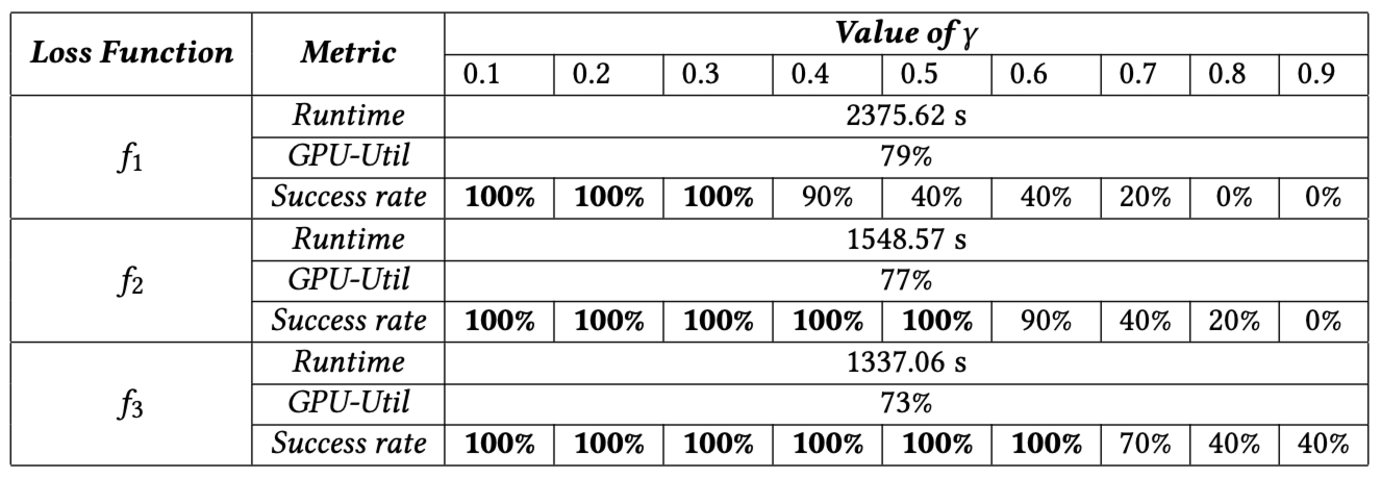
\includegraphics[width=14.0cm]{figures/daedalus-loss-exp.pdf}
\end{center}
\caption{
提案した loss の比較実験.
モデルは YOLO-v3 で MSCOCO2017 validation データからランダムに 10 枚サンプリングして評価している.
Runtime は画像一枚当たりの処理時間である.
success rate は誤った bbox が検出されているかを目視でチェックしている.
図は \cite{wang2019daedalus} より引用.
}
\label{fig:daedalus-loss-exp}
\end{figure}
%

実験の結果は図 \ref{fig:daedalus-result-fp-map} である.
NMS の閾値の値に依らず, FP rate はほぼ 1.0 に, mAP はほぼ 0 に張り付いており, 大量の bbox が誤検出されていることが分かる.
検出された bbox を図示した例が図 \ref{fig:daedalus-example} であり, 表示の問題もあるが元画像が見えなくなるほど bbox で埋め尽くされている.
クラス予測部分ではなく, bbox 検出部分を対象とした攻撃が期待通りに機能していることが示されている.
%
\begin{figure}[htbp]
\begin{center}
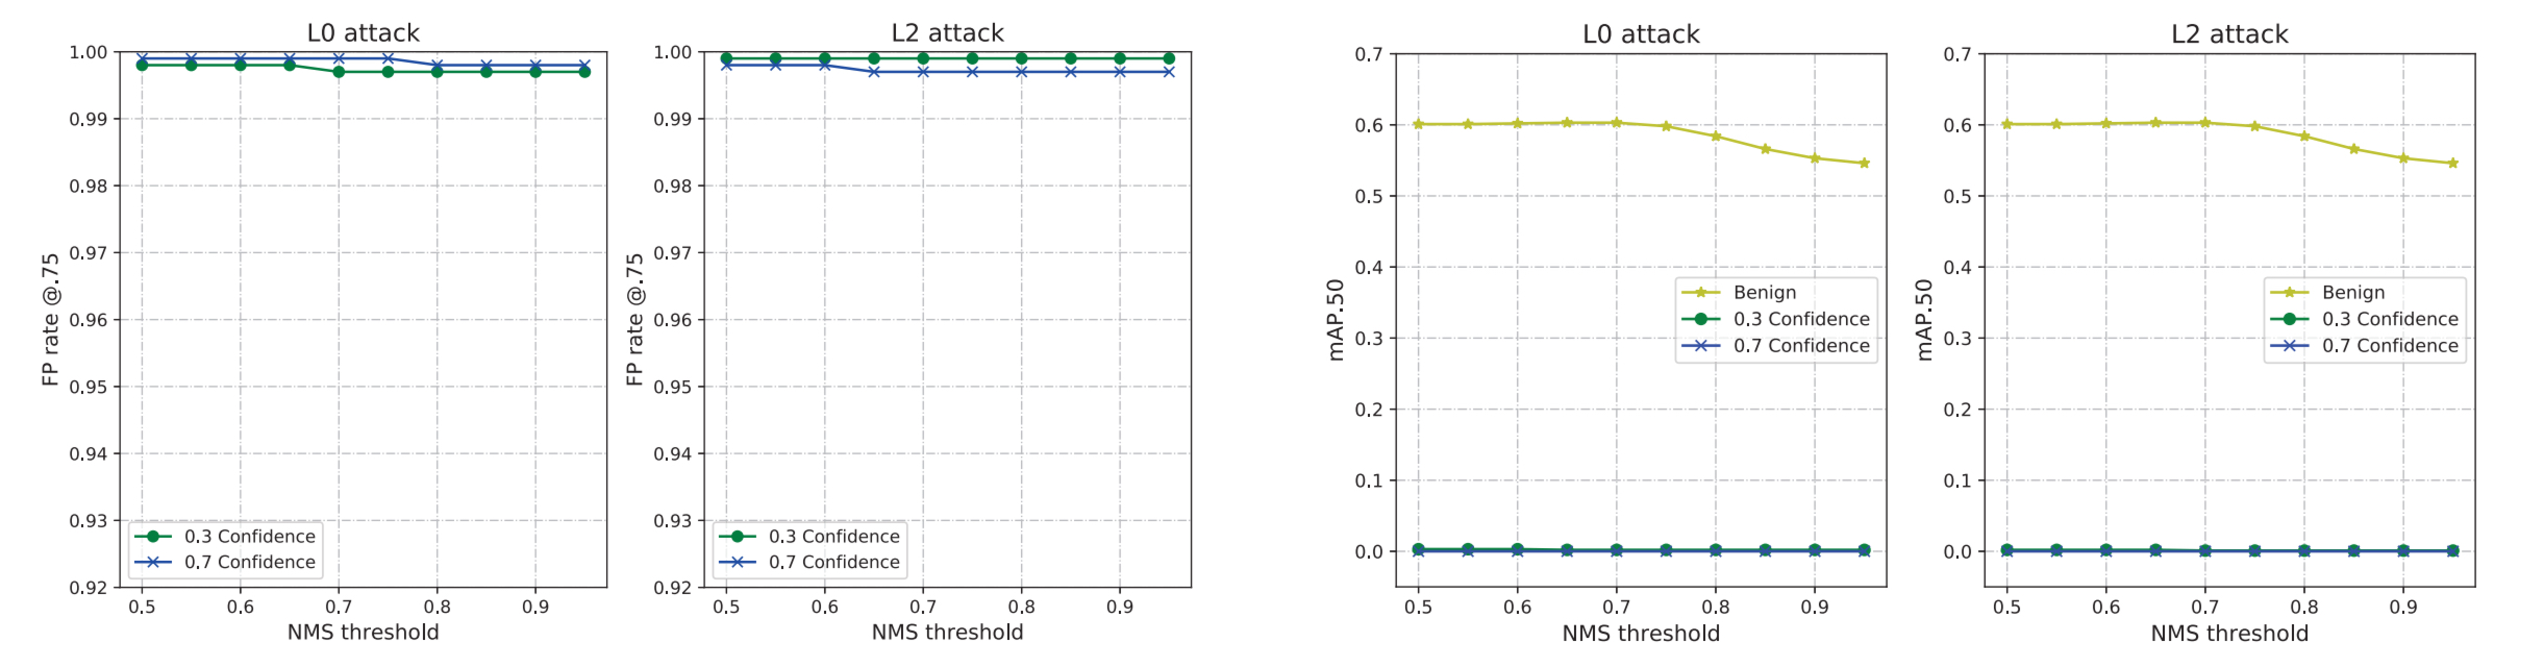
\includegraphics[width=16.0cm]{figures/daedalus-result-fp-map.pdf}
\end{center}
\caption{
モデルは YOLO-v3 で MSCOCO2017 validation データから 100 枚サンプリングして提案手法を検証した結果.
左の二つが FP rate を測定したもので, 右の二つが mAP を測定したものであり, 横軸はどちらも NMS の閾値である.
右の二つの結果は mAP の IoU の IoU 閾値として 0.5 を用いており, 黄色い線の benign は clean データに対する結果である.
図は \cite{wang2019daedalus} より引用.
}
\label{fig:daedalus-result-fp-map}
\end{figure}
%
%
\begin{figure}[htbp]
\begin{center}
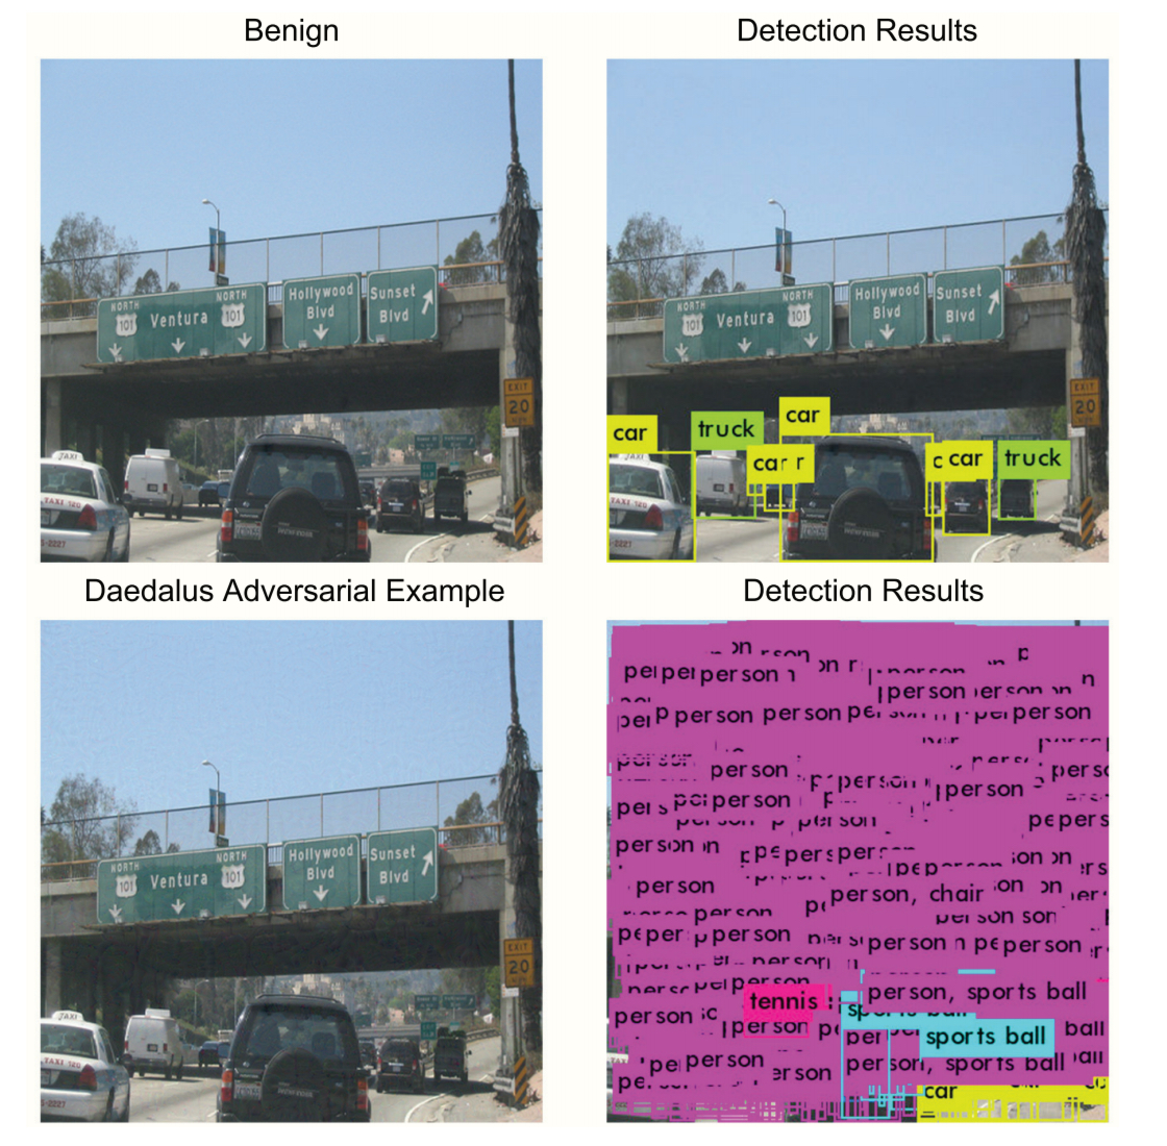
\includegraphics[width=10.0cm]{figures/daedalus-example.pdf}
\end{center}
\caption{
YOLO-v3 に対する攻撃の例.
大量の bbox が誤検出されている.
摂動は拡大すれば目視で確認できなくはないというレベルになっている.
図は \cite{wang2019daedalus} より引用.
}
\label{fig:daedalus-example}
\end{figure}
%

bbox を検出するという処理は detector にとって常に必要なものであり, この論文では adversarial examples の作成を複数モデルのアンサンブルで実施することで, どのモデルに対しても攻撃が成功することも示している.
このアンサンブルは単純に loss の計算を複数モデルの平均にするだけでよい.
detector としてよく使われるものはそれほど種類が多くはないため, アンサンブルによってかなり広範囲を攻撃対象とできる可能性がある.
この手法は digital attack で摂動も画像全体に適用するものであるため, このままでは自動運転などの脅威にはならないが, 方向性として bbox を攻撃するという手法があることを認識しておくことは重要かもしれない.

この手法は, detector の bbox 検出部分に注目して大量の bbox を誤検出させるアルゴリズムを考案したという点が興味深い.
これまでは detector に対する攻撃手法は classifier に対する攻撃手法を拡張するというものが多かったため, detector に対する攻撃に新たな視点をもたらしている.
detector に対する攻撃が様々な観点から進展していくことで, detector の性質がより深く理解されることが期待される.
